\chapter{Návrh užívateľského rozhrania}
\label{navrh ui}

Skôr než začneme aplikáciu programovať, tak si musíme stanoviť ako bude vyzerať. Po~prejdení požiadaviek z~podkap.~\ref{poziadavky} a~prekonzultovaní s~klientom bol vypracovaný návrh užívateľského rozhrania, ktorý si v~tejto kapitole predstavíme. V~požiadavke P1 (Roly užívateľa, viď~\ref{poziadavky}) bolo spomenuté, že budeme chcieť zobrazovať odlišný obsah bežným zákazníkom a~administrátorom. Preto bude následujujúci text rozdelený na~časti podľa pohľadov pre~zákazníka, pre~administrátora, príp.~spoločný pohľad, ktorý je pre~zákazníka a~administrátora rovnaký (ak užívateľ nie je prihlásený, berieme ho ako neprihláseného zákazníka) alebo~pohľad pre~neprihlásených užívateľov.

\section{Hlavné rozloženie aplikácie}
\label{hlavne rozlozenie aplikacie}

\textbf{Spoločný pohľad:} Hlavné rozloženie aplikácie by malo vyzerať tak, že v~hornej ľavej časti by mal byť zobrazený názov firmy (mal by fungovať ako odkaz na~domovskú stránku) a~vpravo hore by malo byť zobrazené telefónne číslo firmy (malo by fungovať ako odkaz na~sekciu~Kontakt). Pre~lepšiu predstavu hlavného rozloženia aplikácie viď~obr.~\ref{layout}.

\begin{figure}[H]\centering
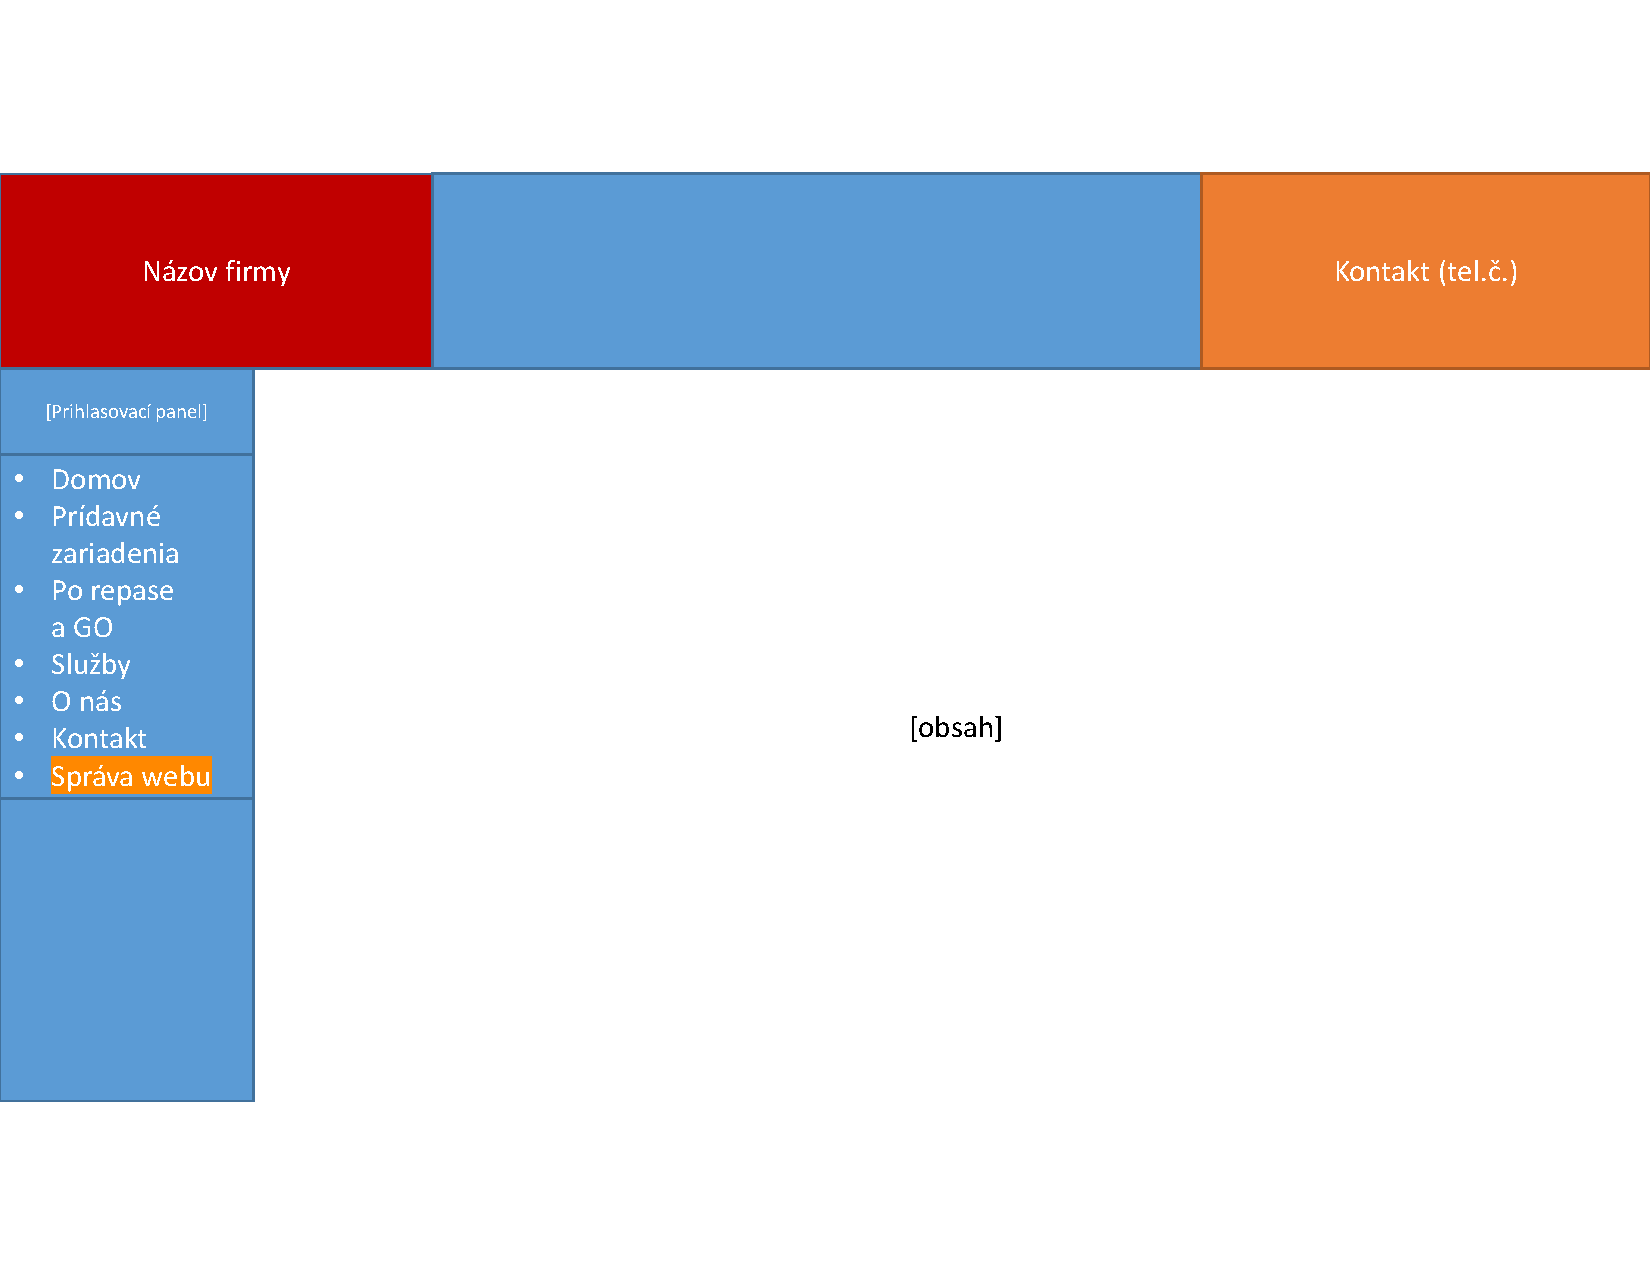
\includegraphics[width=140mm]{../img/UI concept/layout}
\caption{Návrh rozloženia aplikácie}
\label{layout}
\end{figure}

V~ľavej časti by mala byť zobrazená navigácia. V~navigácii by sa mali nachádzať odkazy~,,Domov``, ,,Prídavné zariadenia``, ,,Po~repase a~GO``, ,,Služby``, ,,O~nás``, ,,Kontakt`` a~,,Kontakt``. Nad~navigáciou by sa mal nachádzať prihlasovací panel, o~ktorom si viac povieme v~podkapitole~\ref{splnenie p6}.

Ďalej v~centre aplikácie by mal byť obsah (viď~obsahovú časť v~centre obr.~\ref{layout}), ktorý by sa mal meniť podľa toho v~akej časti aplikácie sa užívateľ nachádza. Všetky obrázky v~následujúcich podkapitolách (s~výnimkou grafov prechádzania medzi časťami aplikácie a~modálnym oknom, o~ktorom si povieme v~následujúcej podkapitole) budú predstavovať obsahovú časť ak sa explicitne nepovie inak.\\

\textbf{Pohľad pre~administrátrov:} Bolo spomenuté, že v~navigácii by sa mali nachádzať odkazy~,,Domov``, ,,Prídavné zariadenia``, ,,Po~repase a~GO``, ,,Služby``, ,,O~nás``, ,,Kontakt`` a~,,Kontakt``. Okrem týchto odkazov by mal mať administrátor zobrazený aj odkaz~,,Správa webu``.

\section{Modálne potvrdzovacie okno}
\label{modalne potvrdzovacie okno}

\textbf{Spoločný pohľad:} \href{https://ux.stackexchange.com/questions/12045/what-is-a-modal-dialog-window}{Modálne okno} je vyskakovacie dialógové okno, ktoré núti užívateľa k~interakcii s~ním. Kým užívateľ nevykoná interakciu s~oknom, nemôže interagovať s~rodičovkou aplikáciou (rodičovským oknom).

V~následujúcich podkapitolách bude v~spojení s~mazaním položiek viackrát spomenuté modálne potvrdzovacie okno. Pre~jeho lepšiu predstavu viď~obr.~\ref{confirmation modal}.

\begin{figure}[H]\centering
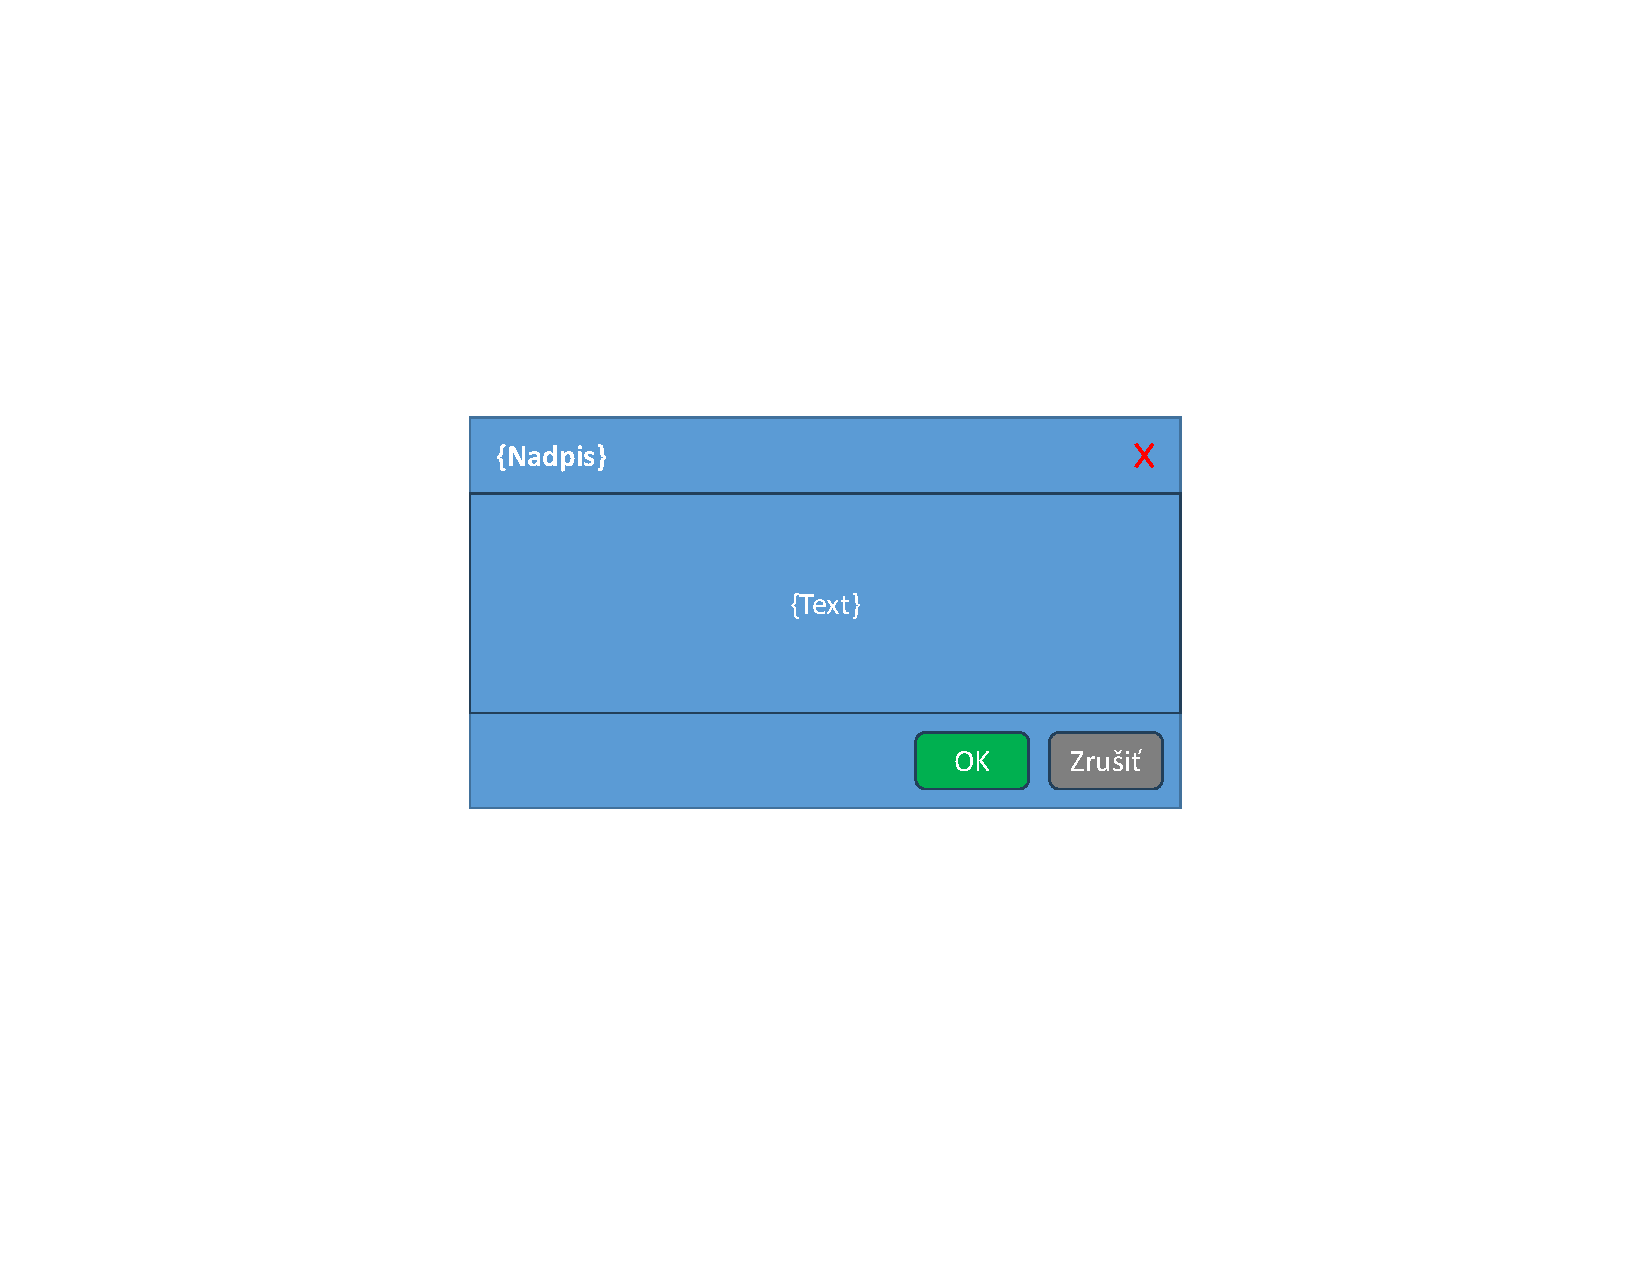
\includegraphics[width=140mm]{../img/UI concept/confirmation modal}
\caption{Potvrdzovacie modálne okno.}
\label{confirmation modal}
\end{figure}

Okno by malo obsahovať vo~vrchnej časti nadpis a~v~centre text oznamujúci akciu. V~spodnej časti by sa mali nachádzať tlačidlá~,,OK`` (pre~potvrdenie akcie) a~,,Zrušiť`` (pre~zrušenie akcie).

\section{Sekcie Podmienky používania a Zásady ochrany osobných údajov}
\label{gdpr}

Z požiadaviek P6 (užívateľ sa môže zaregistrovvať do systému, a~tým poskytnuť systému svoje údaje), P3 a P8 (užívateľ poskytuje osobné informácie pri odosielaní dopytu), P4 a P5 (užívateľ ponúka sumy do~aukcie a~následne po~vyhodnotení aukcie môžu byť jeho údaje zverejnené v~rozposlaných emailoch) vieme, že systém má zhromažďovať a~pracovať s~užívateľskými údajmi. Preto by bolo vhodné systém pripraviť na splnenie \href{https://www.uoou.cz/obecne-narizeni-o-ochrane-osobnich-udaju-gdpr/ds-3938/p1=3938}{GDPR}. GDPR predstavuje regulácie na ochranu užívateľa pred~zneužitím jeho údajov.

Pre splnenie GDPR by bolo dobré vyhradiť časti aplikácie, kde sa budú môcť vložiť texty ohľadom podmienok používania aplikácie a zásad ochrany osobných údajov vyhotovené právnickou osobou. Pre lepšiu predstavu týchto častí aplikácie viď obr. \ref{gdpr1} a \ref{gdpr2}.

\begin{figure}[H]\centering
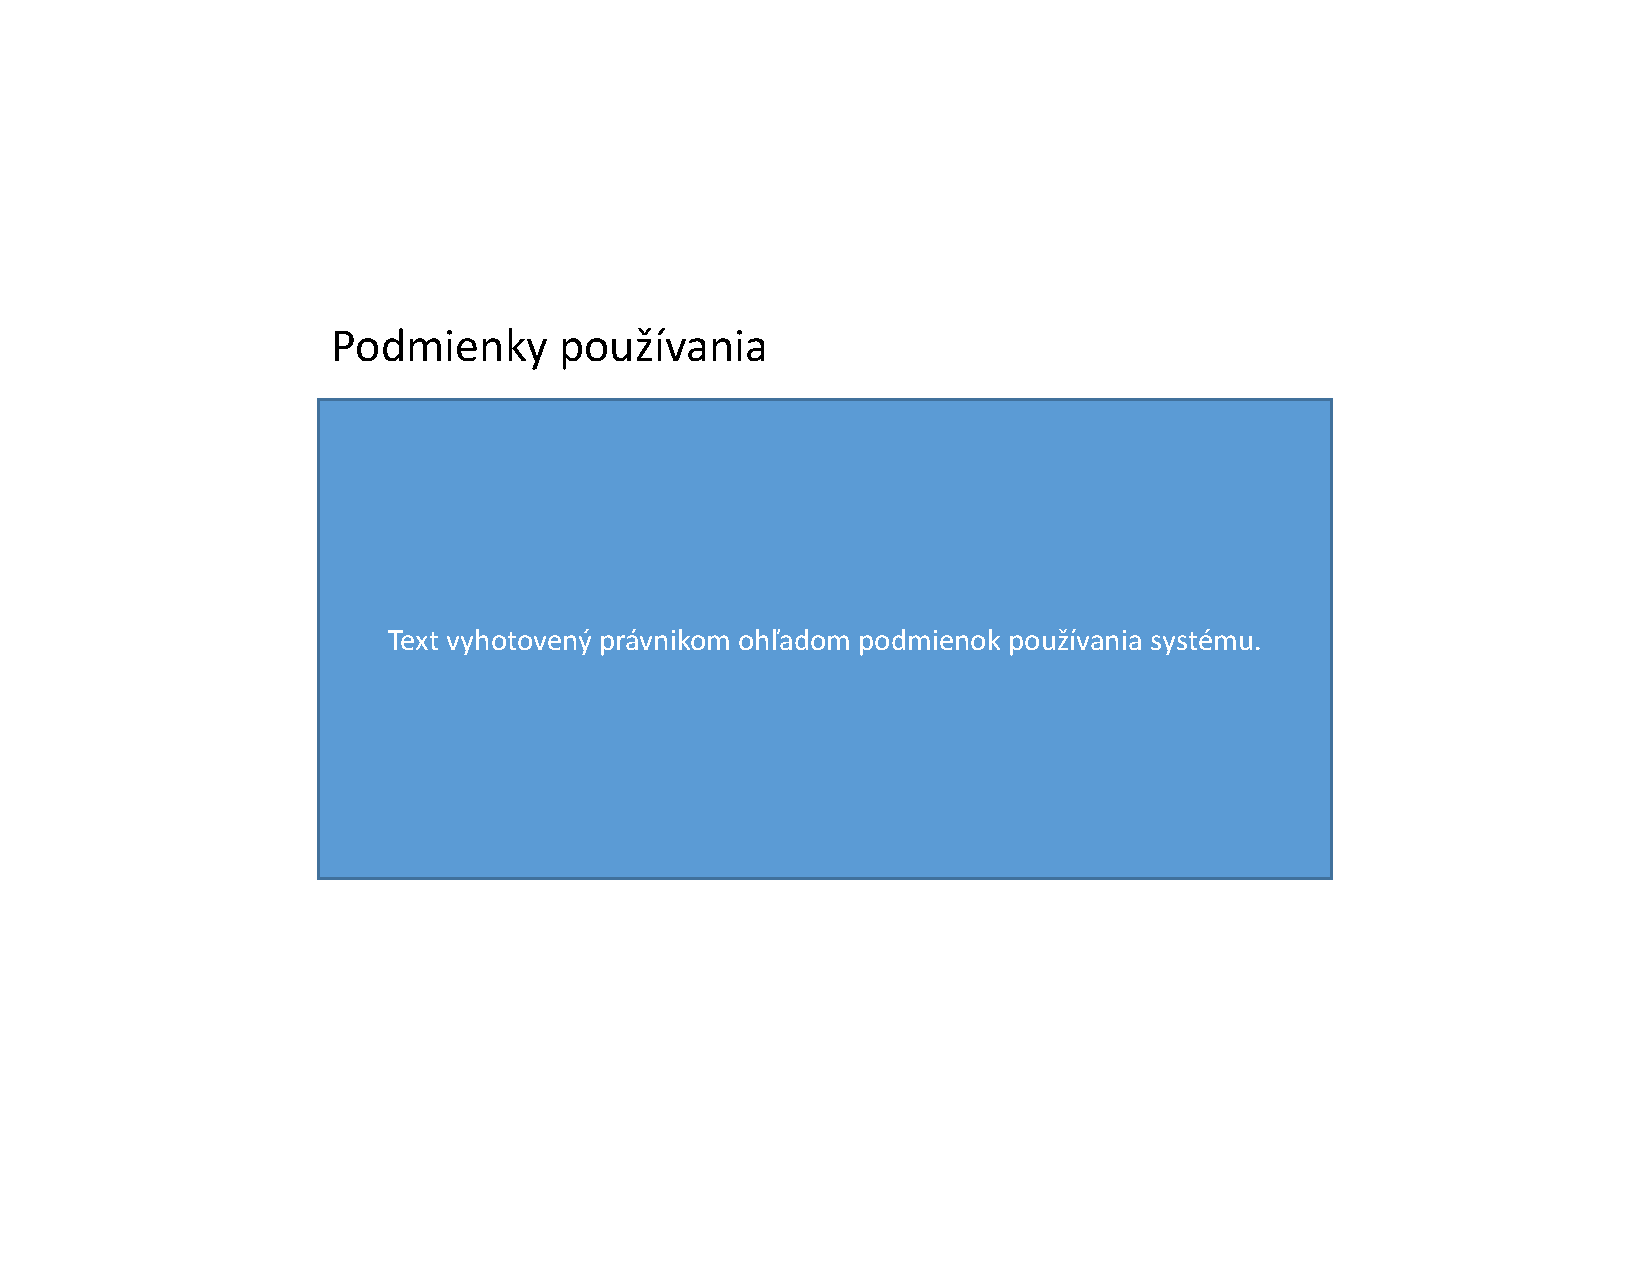
\includegraphics[width=140mm]{../img/UI concept/gdpr1}
\caption{Časť aplikácie s podmienkami používania.}
\label{gdpr1}
\end{figure}

\begin{figure}[H]\centering
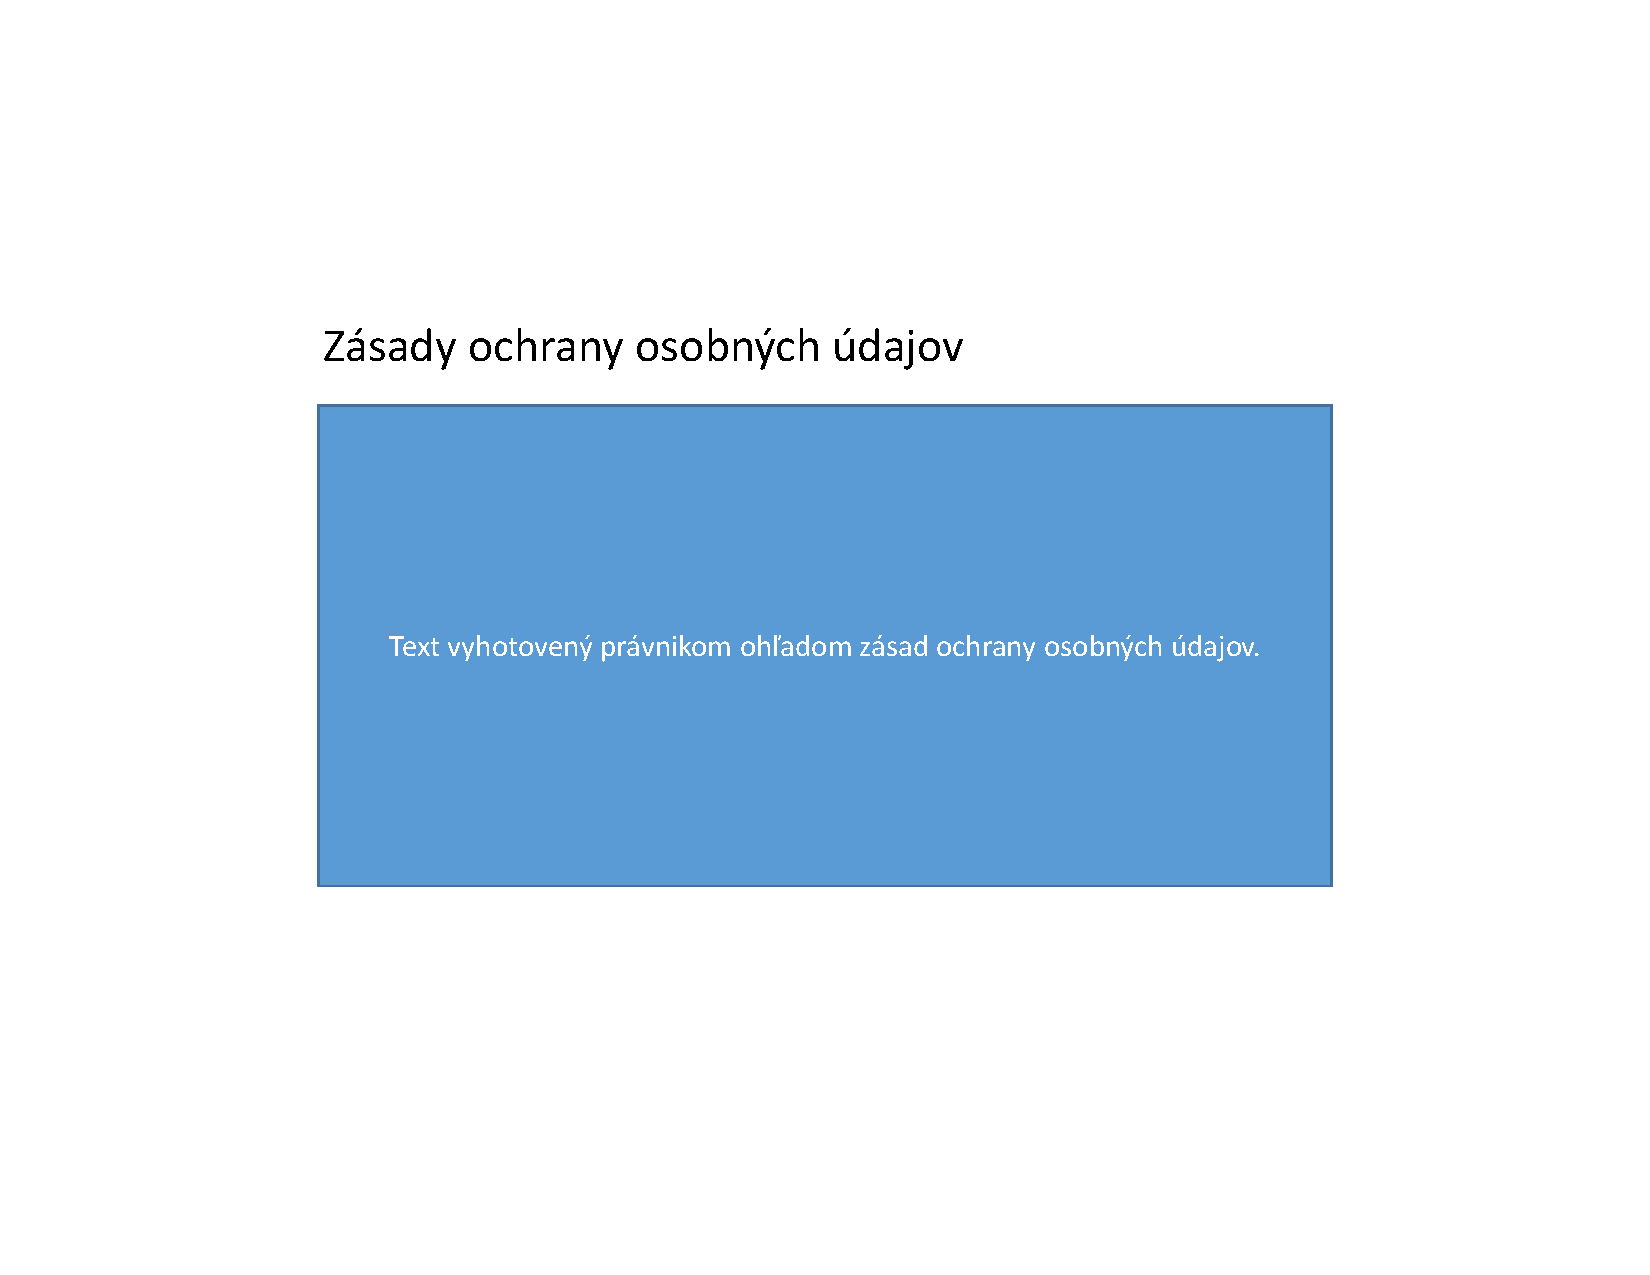
\includegraphics[width=140mm]{../img/UI concept/gdpr2}
\caption{Časť aplikácie so zásadami ochrany osobných údajov.}
\label{gdpr2}
\end{figure}

V časti aplikácie s podmienkami používania by mal byť nadpis \uv{Podmienky používania}. V časti aplikácie so zásadami ochrany osobných údajov by mal byť nadpis \uv{Zásady ochrany osobných údajov}. V prípade oboch častí aplikácie platí, že pod názvom by sa mal nachádzať text vyhotovený právnickou osobou na danú tému.

Na tieto časti aplikácie by sa malo odkazovať pri registrácii užívateľa, pri odosielaní dopytu z detaila bagra, detaila prídavného zariadenia alebo zo sekcie Služby, podobne pri ponúkaní sumy do aukcie z detailu aukčnej ponuky. Viac si o týchto častiach aplikácie povieme v následujúcom texte.

Okrem toho by mal systém umožniť užívateľovi vymazať svoje dáta zo~systému, a~taktiež ich na~vyžiadanie exportovať. Toto sa splní v~časti aplikácie s~profilom užívateľa, ale~o~nej si povieme viac v~časti Profil (viď~\ref{profil}).

\section{Splnenie P2 a P3}

V~tejto podkapitole si prejdeme časti aplikácie splňujúce požiadavky P2 a~P3, t.~j.~predstavenie hlavnej ponuky, bagrov, prídavných zariadení, a~takisto si z~časti ukážeme ako môže administrátor jednotlivé položky vytvárať, upravovať a~vymazovať (z~časti preto, lebo v~prípade bagrov si neskôr ukážeme aj iný spôsob). Každá časť aplikácie, ktorú si spomenieme v tejto časti textu, a ktorú môžeme vidieť na obr. \ref{p2 p3 graph}, si opíšeme detailnejšie neskôr v následujúcoch častiach textu.

\begin{figure}[H]\centering
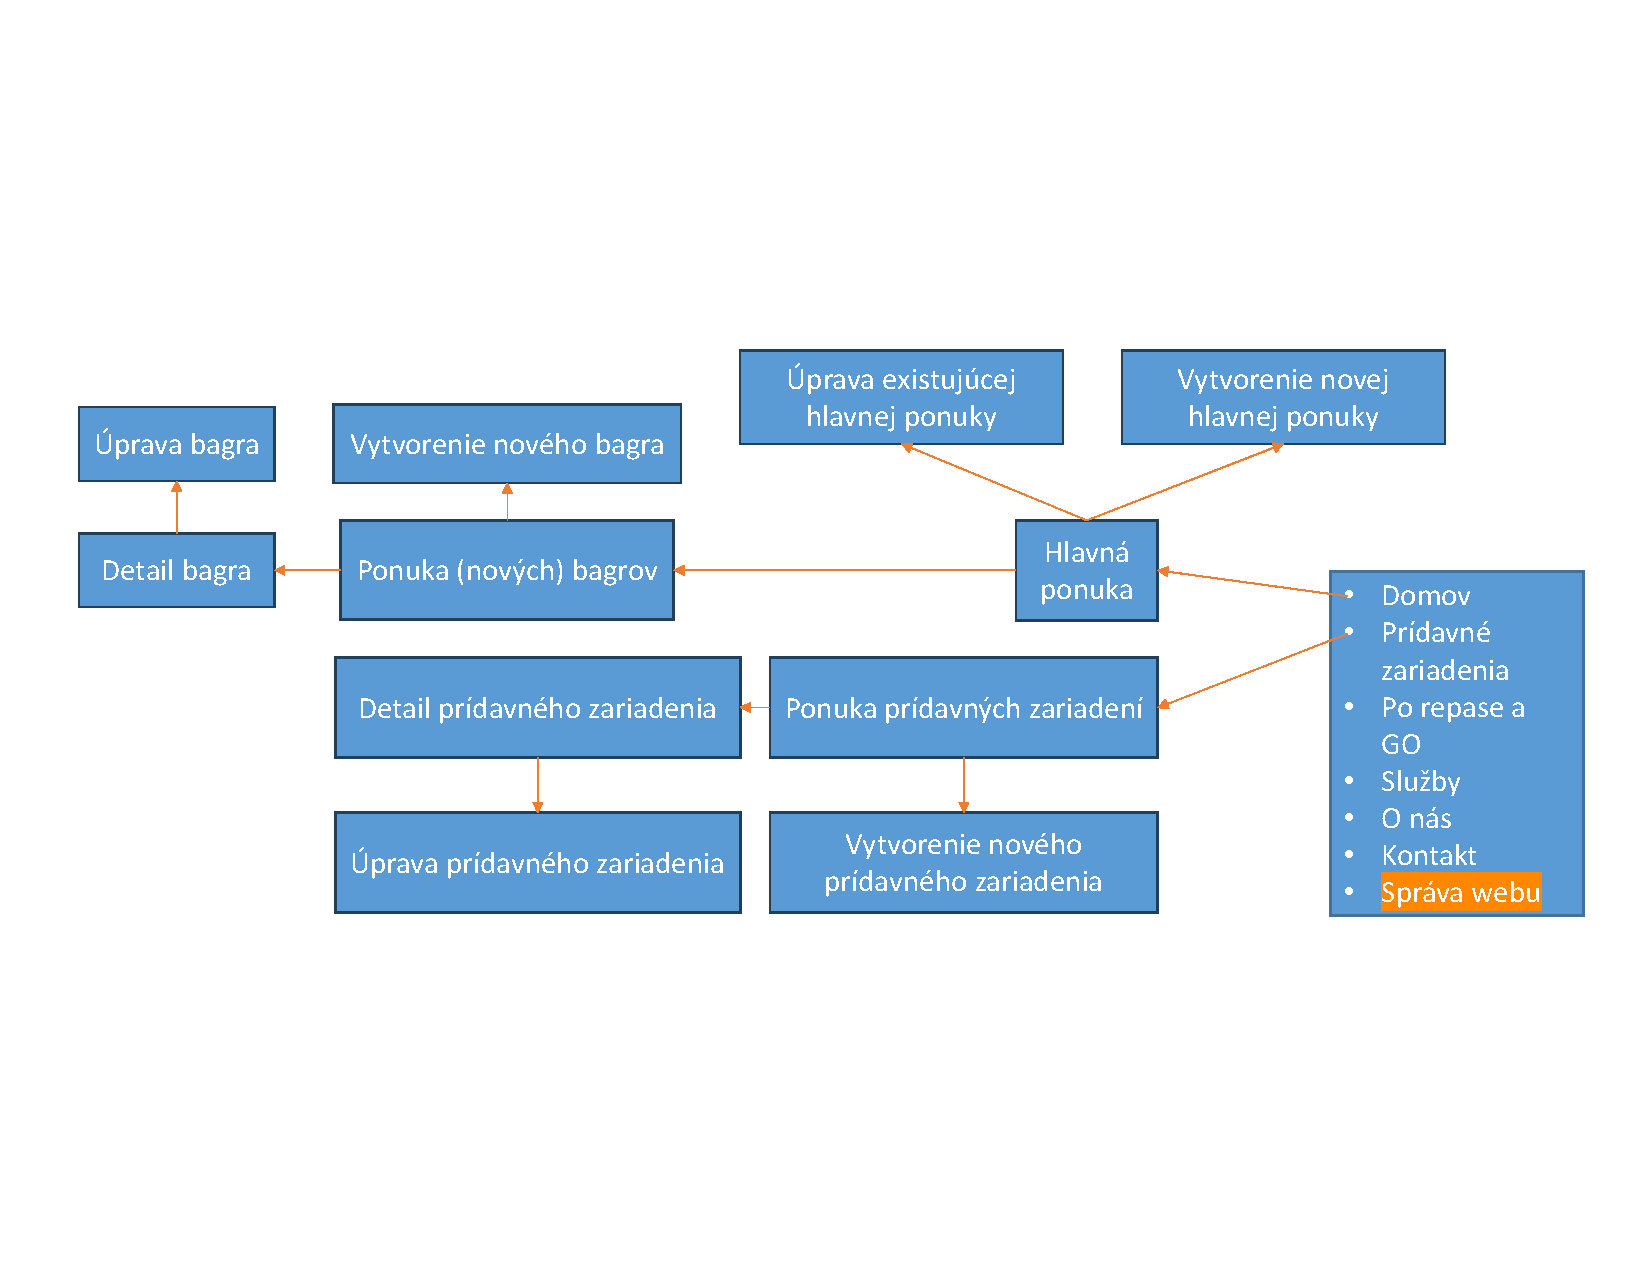
\includegraphics[width=140mm]{../img/UI concept/p2 p3 graph}
\caption{Prechádzanie medzi časťami aplikácie spĺňajúcimi požiadavky P2 a~P3.}
\label{p2 p3 graph}
\end{figure}

\textbf{Spoločný pohľad:} Pre~lepšie pochopenie prechádzania medzi jednotlivými časťami programu viď~obr.~\ref{p2 p3 graph}. Pri~prvotnom príchode do~aplikácie (alebo~po~kliknutí na~odkaz~,,Domov`` v~navigácii, viď hranu 1 na obr. \ref{p2 p3 graph}) má byť užívateľovi zobrazená sekcia Hlavná ponuka s~vylistovanými kartami hlavnej ponuky.

Na~každej karte hlavnej ponuky by malo byť tlačidlo ,,Zobraziť``, ktoré by malo užívateľa presmerovať k~vylistovaným kartám (nových) bagrov~-- Ponuka (nových) bagrov (viď hranu 2 na obr. \ref{p2 p3 graph}). Kliknutím na~nejakú z~kariet bagrov by mal byť užívateľ presmerovaný do~časti aplikácie zobrazujúcej detail vybraného bagra (viď hranu 3 na obr. \ref{p2 p3 graph}).

Podobne by mal byť užívateľ schopný kliknúť na~odkaz ,,Prídavné zariadenia`` v~navigácii, ktorý by ho mal presmerovať na~vylistované karty prídavných zariadení~-- Ponuka prídavných zariadení (viď hranu 4 na obr. \ref{p2 p3 graph}). Ak užívateľ klikne na~nejakú z~kariet, mal by byť presmerovaný na~detail vybraného prídavného zariadenia (viď hranu 5 na obr. \ref{p2 p3 graph}).

\textbf{Pohľad pre~zákazníkov:} V~časti s~detailom bagra by sa mal nachádzať dopytový formulár, ktorý by mal obsahovať odkaz do~časti aplikácie s~podmienkami používania (viď hranu 12 na obr. \ref{p2 p3 graph}). Okrem neho by sa mal vo formulári nachádzať odkaz do časti so zásadami ochrany užívateľských údajov (viď hranu 13 na obr. \ref{p2 p3 graph}).

V~časti s~detailom prídavného zariadenia by sa mal nachádzať dopytový formulár, ktorý by mal obsahovať odkaz do~časti aplikácie s~podmienkami používania (viď hranu 14 na obr. \ref{p2 p3 graph}). Okrem neho by sa mal vo formulári nachádzať odkaz do časti so zásadami ochrany užívateľských údajov viď hranu 15 na obr. \ref{p2 p3 graph}.

\textbf{Pohľad pre~administrátorov:} Administrátorovi by sa na~každej z~kariet hlavnej ponuky malo zobrazovať tlačidlo~\uv{E}, ktoré by ho malo po~kliknutí presmerovať do~časti aplikácie, kde by mohol danú ponuku upravovať (viď hranu 6 na obr. \ref{p2 p3 graph}). Takisto by sa mal v~sekcii Domov nachádzať nad~kartami odkaz, ktorý by mal po~kliknutí administrátora presmerovať do~časti aplikácie, kde by mal byť schopný vytvoriť novú hlavnú ponuku (viď hranu 7 na obr. \ref{p2 p3 graph}).

V~časti s~vylistovanými bagrami (Ponuka (nových) bagrov) by sa mal nachádzať odkaz, ktorý by po~kliknutí presmeroval administrátora do~časti aplikácie, kde by mohol vytvoriť nový bager (viď hranu 8 na obr. \ref{p2 p3 graph}). Ďalej z~časti aplikácie zobrazujúcej detail bagra by sa mal byť administrátor schopný dostať kliknutím na~tlačidlo ,,Upraviť`` do~časti aplikácie umožňujúcej upravovanie daného bagra (viď hranu 9 na obr. \ref{p2 p3 graph}).

V~časti s~vylistovanými prídavnými zariadeniami (Ponuka prídavných zariadení) by sa mal nachádzať odkaz, ktorý by po~kliknutí presmeroval administrátora do~časti aplikácie, kde by mohol vytvoriť nové prídavné zariadenie (viď hranu 10 na obr. \ref{p2 p3 graph}). Ďalej z~časti aplikácie zobrazujúcej detail prídavného zariadenia by sa mal byť administrátor schopný dostať kliknutím na~tlačidlo ,,Upraviť`` do~časti aplikácie umožňujúcej upravovanie daného prídavného zariadenia (viď hranu 11 na obr. \ref{p2 p3 graph}).

\subsection{Hlavná ponuka}
\label{hlavna ponuka}

\textbf{Spoločný pohľad:} Po~príchode do~aplikácie by sa mal užívateľ ocitnúť v~domovksej časti aplikácie, kde by mali byť zobrazené karty hlavných ponúk. Pre~lepšiu predstavu viď~obr.~\ref{main offer cards}.

\begin{figure}[H]\centering
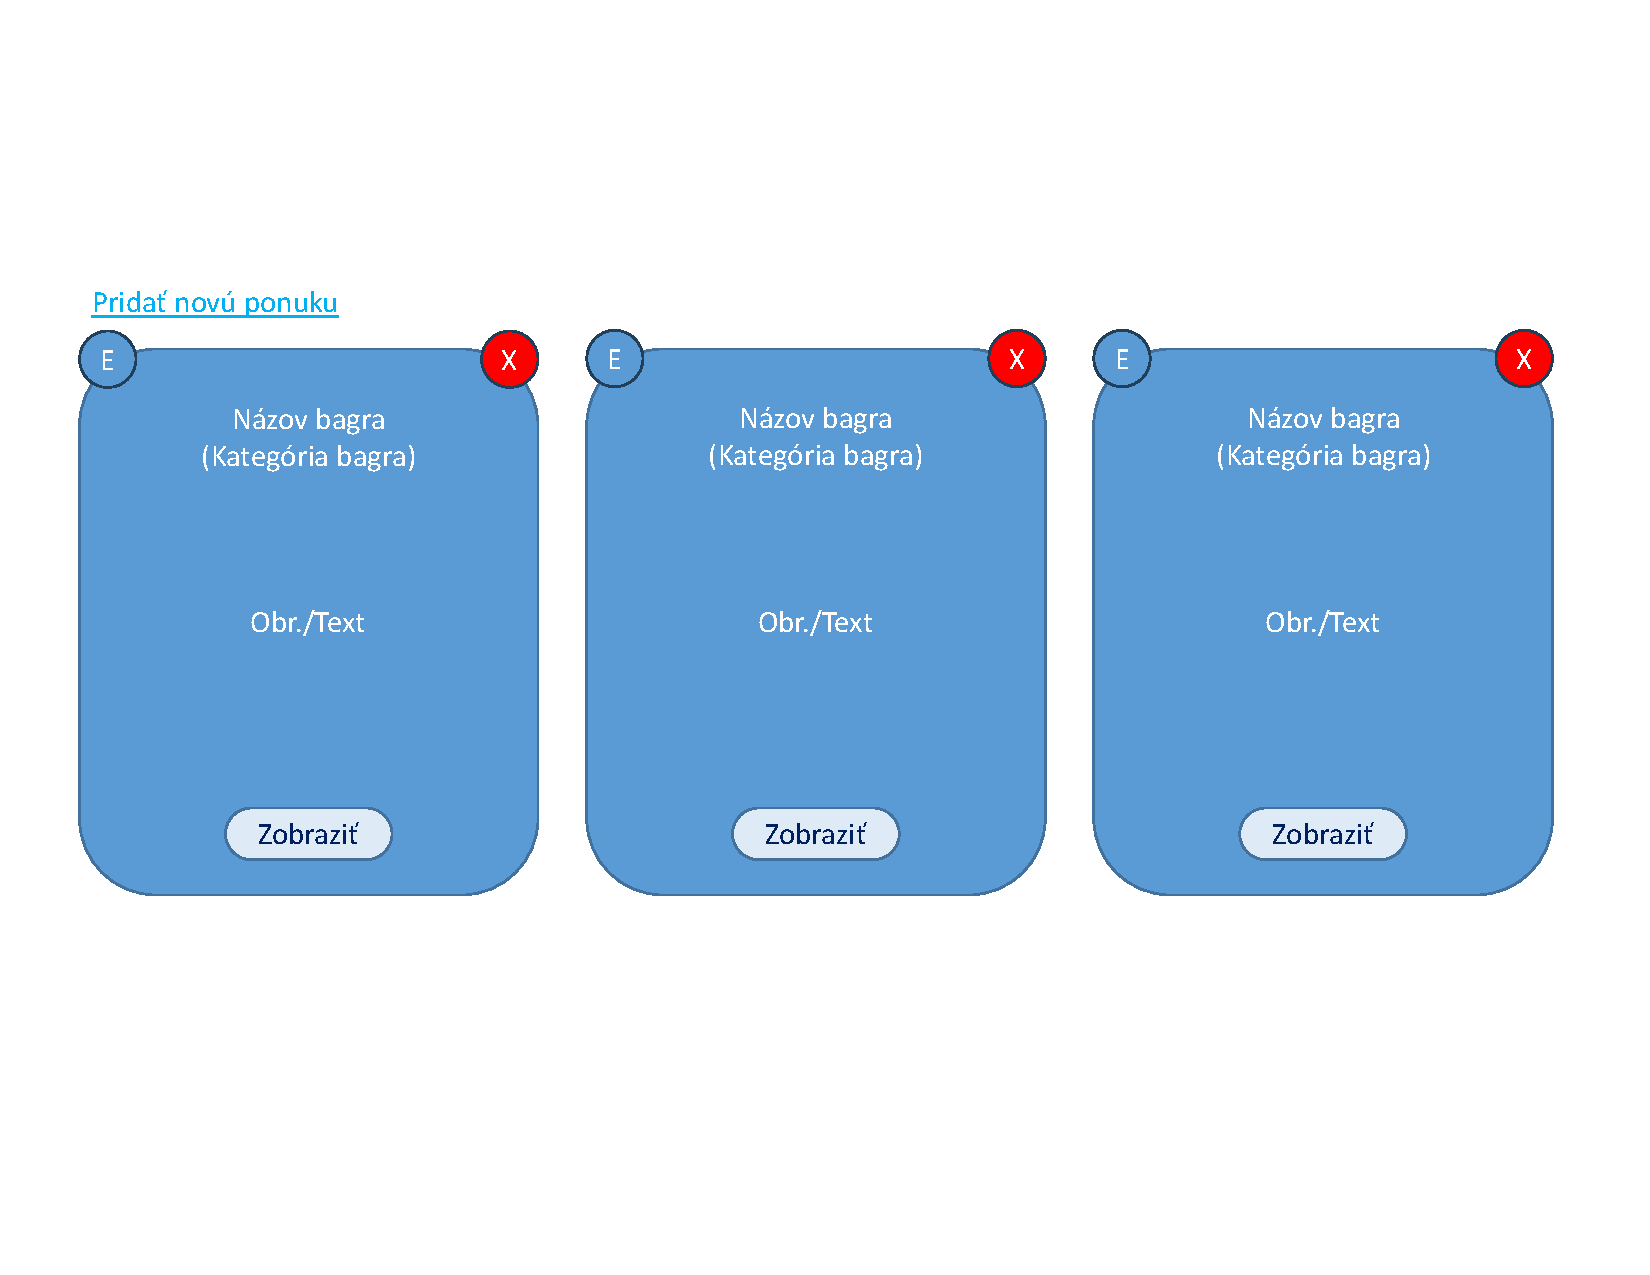
\includegraphics[width=140mm]{../img/UI concept/main offer cards}
\caption{Hlavná ponuka (domovská časť aplikácie).}
\label{main offer cards}
\end{figure}

Každá z~kariet by mala zobrazovať fotku reprezentujúcu danú ponuku (resp.~typ bagra, ktorý je určený kombináciou kategórie a~značky bagra ako bolo spomenuté v~požiadavke P2.1., viď~podkap.~\ref{poziadavky}). Ak užívateľ prejde kurzorom na~kartu, tak by sa mal namiesto fotky zobraziť text opisujúci danú ponuku. Každá karta by mala obsahovať tlačidlo~,,Zobraziť``, ktoré by malo užívateľa po~kliknutí presmerovať k~ponuke (nových) bagrov typu, ktorý prezentuje daná hlavná ponuka.

\textbf{Pohľad pre~administrátorov:} Na~každej karte hlavnej ponuky by mali byť zobrazené tlačidlá ,,E`` a~,,X`` vo~vrchných rohoch kariet, a~takisto nad~vylistovanými kartami odkaz ,,Pridať novú ponuku``. Po~kliknutí na~tlačidlo ,,E`` nejakej z~hlavných ponúk by mal byť administrátor presmerovaný na~formulár vyplnený údajmi danej hlavnej ponuky, kde by mohol túto ponuku upravovať. Tlačidlo ,,X`` by malo slúžiť na~vymazanie danej hlavnej ponuky, po~kliknutí naň by sa malo zobraziť modálne potvrdzovacie okno s~nadpisom~,,Vymazať ponuku natrvalo`` a~textom \uv{Naozaj chcete túto ponuku vymazať natrvalo?}. Ďalej po~kliknutí na~odkaz ,,Pridať novú ponuku`` by mal byť administrátor presmerovaný na~prázdny formulár, kde bude môcť vytvoriť novú hlavnú ponuku.

\subsection{Vytvorenie novej a~úprava existujúcej hlavnej ponuky}
\label{vytvorenie novej a uprava existujucej hlavnej ponuky}

\textbf{Pohľad pre~administrátorov:} Ako bolo v~predošlej časti spomenuté, administrátor by mal byť schopný z~domovskej časti (časť aplikácie, kde majú byť vylistované hlavné ponuky) kliknutím na~odkaz ,,Pridať novú ponuku`` vytvoriť novú hlavnú ponuku a~kliknutím na~tlačidlo ,,E`` existujúcu hlavnú ponuku upravovať. Pre~lepšiu predstavu tejto časti viď~obr.~\ref{main offer form}.

\begin{figure}[H]\centering
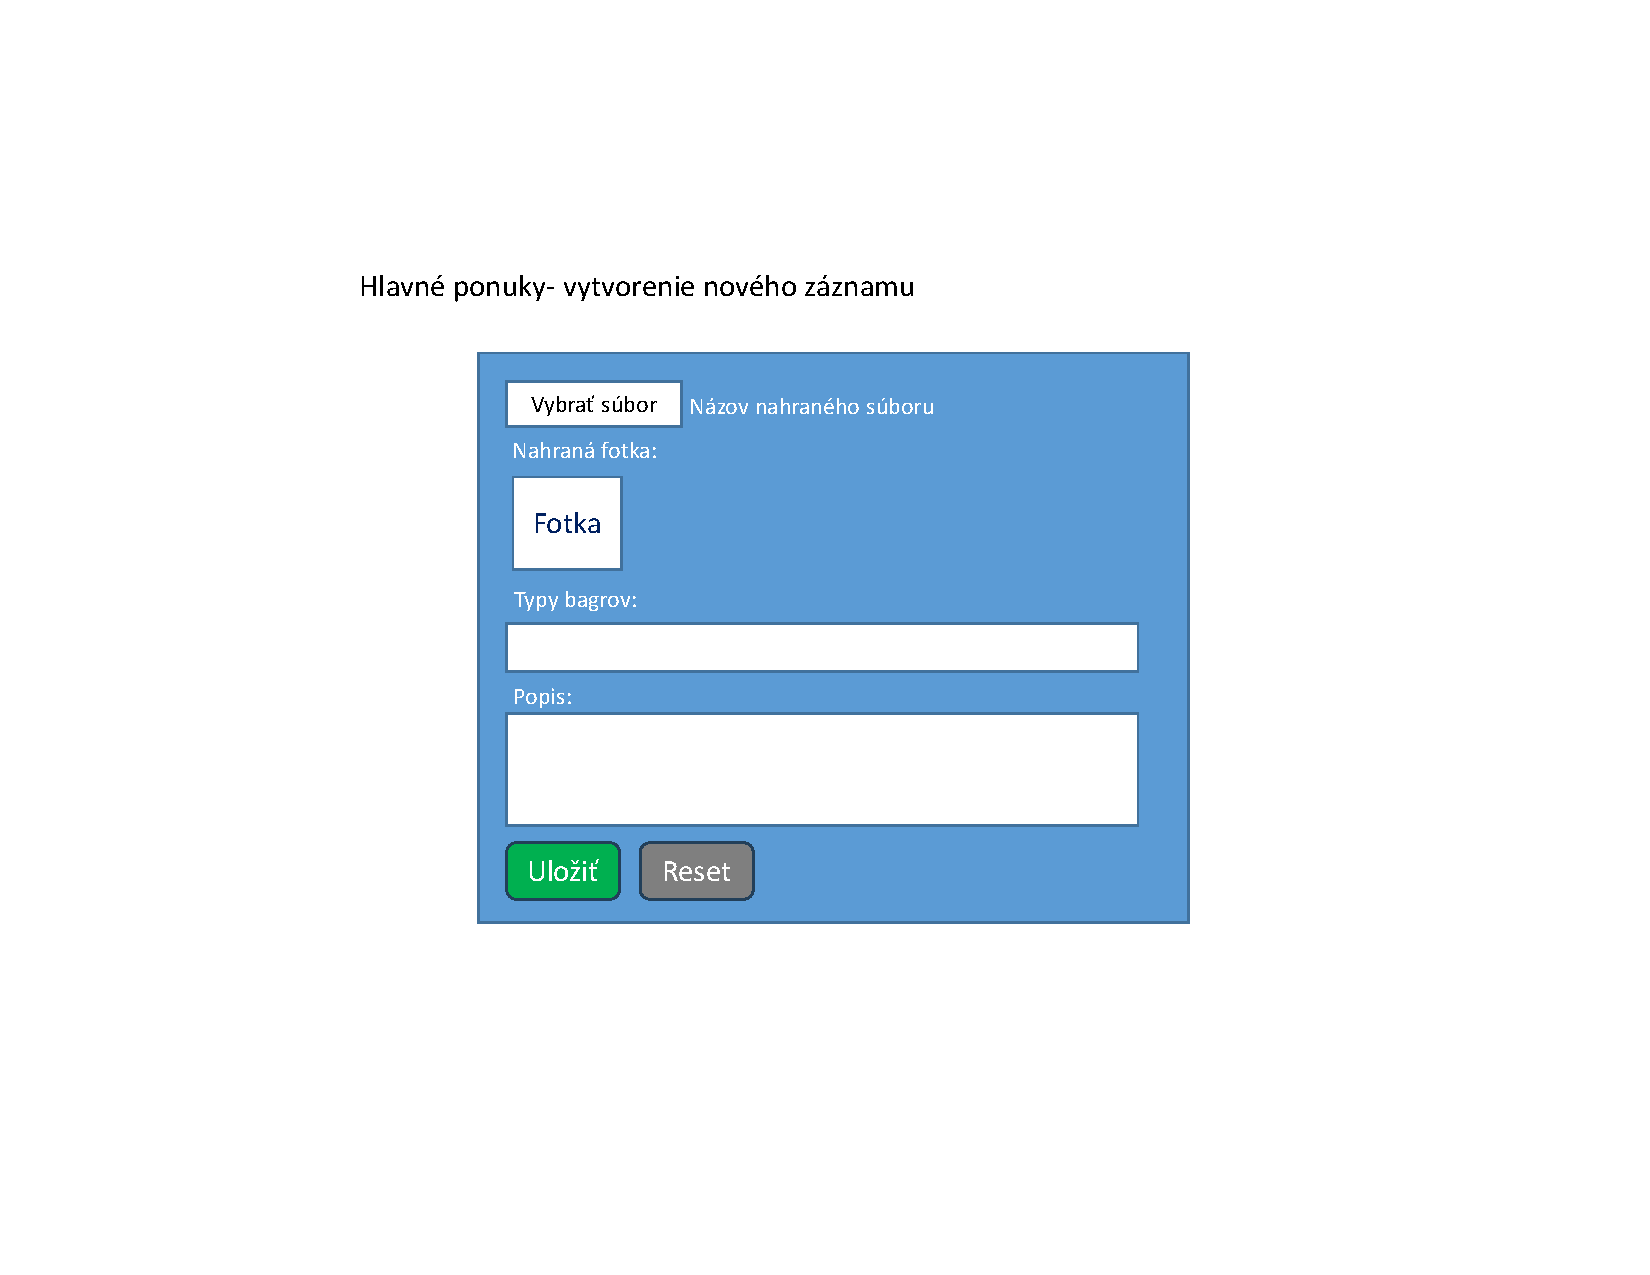
\includegraphics[width=140mm]{../img/UI concept/main offer form}
\caption{Časť aplikácie pre~vytvorenie hlavnej ponuky.}
\label{main offer form}
\end{figure}

Či už v~prípade vytvárania novej, alebo~upravovania existujúcej hlavnej ponuky, by mal byť administrátor presmerovaný do~časti aplikácie s~formulárom umožňujúcim vložiť jednu fotku, vybrať z~možností typov bagrov, a~takisto napísať popis hlavnej ponuky. Všetky údaje až na~popis majú byť povinné. Navyše po~vložení by sa mali fotka a~jej názov zobraziť vo~formulári.

Formulár by mal obsahovať tlačidlá ,,Uložiť`` (na~uloženie hlavnej ponuky) a~tlačidlo~,,Reset`` (na~vyprázdenie formulára). Ak sú po~kliknutí na~tlačidlo~,,Uložiť`` povinné údaje nevyplnené, tak by mal na~to systém administrátora upozorniť prostrednictvom chybových správ pri~jednotlivých poliach.

Ďalej nad~formulárom by mal byť v~prípade vytvárania novej hlavnej ponuky nadpis~,,Hlavné ponuky~-- vytvorenie nového záznamu``. V~prípade úpravy existujúcej hlavnej ponuky by tam mal byť nadpis~,,Hlavné ponuky~-- úprava existujúceho záznamu``.

\subsection{Ponuka (nových) bagrov}
\label{ponuka novych bagrov}

\textbf{Spoločný pohľad:} Po~kliknutí na~tlačidlo ,,Zobraziť`` nejakej z~hlavných ponúk by sa mali užívateľovi vylistovať karty strojov typu, ktorý prezentovala vybraná hlavná ponuka (viď obr.~\ref{excavator cards}). Medzi vylistovanými bagrami nemajú byť bagre určené iba pre~aukciu.

\begin{figure}[H]\centering
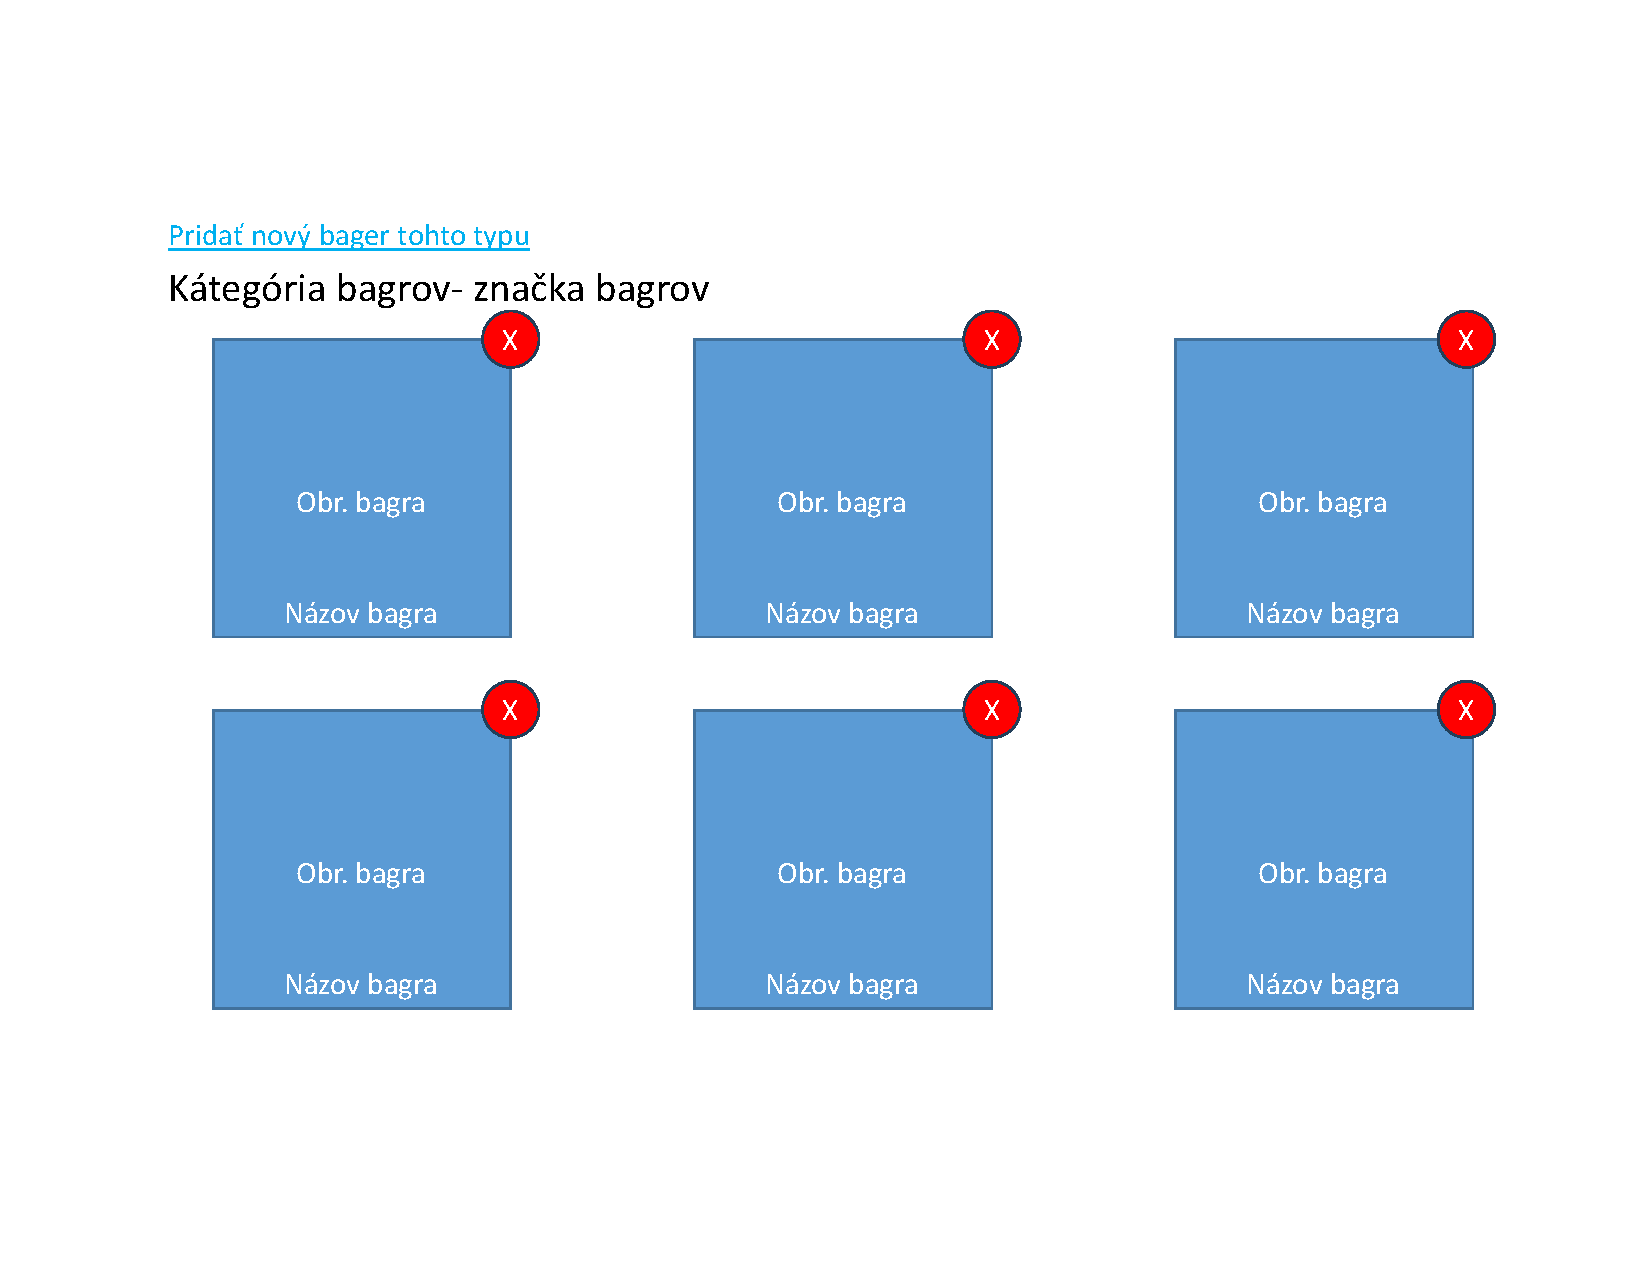
\includegraphics[width=140mm]{../img/UI concept/excavator cards}
\caption{Ponuka bagrov.}
\label{excavator cards}
\end{figure}

Nad~kartami bagrov by sa mal nachádzať nadpis v~tvare ,,\{Kategória vybraného typu bagrov\}~-- \{Značka vybraného typu bagrov\}`` (typ bagra určuje jeho kategóriu a~značku). Po~kliknutí na~nejakú z~kariet by mal byť užívateľ presmerovaný na~detail bagra.

\textbf{Pohľad pre~administrátorov:} Vo~vrchnej časti by sa mal nachádzať odkaz~,,Pridať nový bager``, ktorý by mal užívateľa po~kliknutí presmerovať k~formuláru pre~vytvorenie nového stroja. Ak sa administrátor dostal k~formuláru touto cestou, mal by mať vo~formulári predvyplnený typ stroja podľa typu vylistovaných strojov.

Každá z~kariet by mala mať v~pravom hornom rohu tlačidlo~,,X``, ktoré umožní daný stroj vymazať. Po~kliknutí naň by sa malo zobraziť modálne potvrdzovacie okno s~nadpisom~,,Vymazať bager natrvalo`` a~textom~\uv{Naozaj chcete tento bager vymazať natrvalo?}.

\subsection{Ponuka prídavných zariadení}
\label{ponuka pridavnych zariadeni}

\textbf{Spoločný pohľad:} Po kliknutí na~,,Prídavné zariadenia`` v~navigácii (viď~vľavo na~obr.~\ref{layout}) by sa mali užívateľovi vylistovať karty prídavných zariadení. Pre~lepšiu predstavu tejto časti aplikácie viď~obr.~\ref{additional equipment cards}.

\begin{figure}[H]\centering
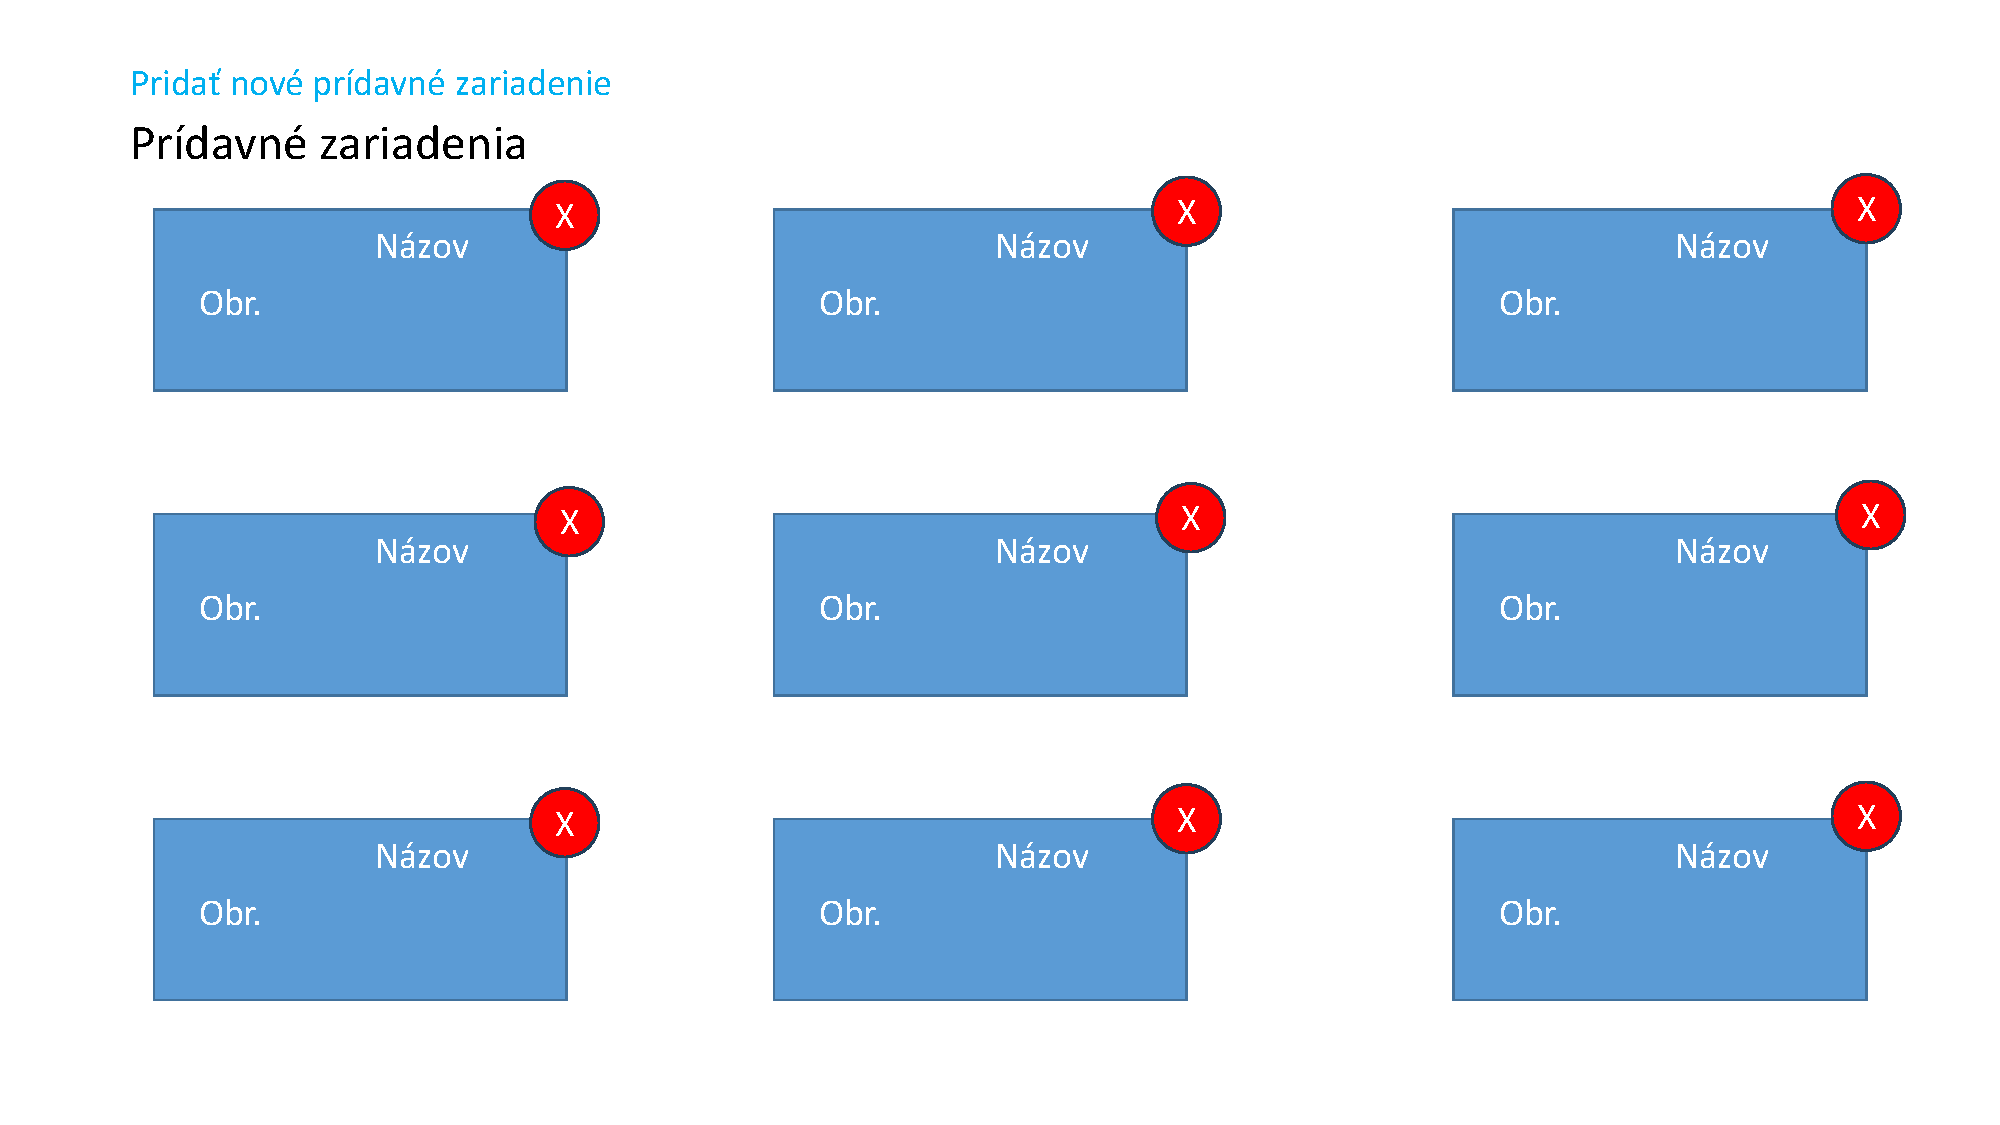
\includegraphics[width=140mm]{../img/UI concept/additional equipment cards}
\caption{Ponuka prídavných zariadení}
\label{additional equipment cards}
\end{figure}

Nad~kartami prídavných zariadení by sa mal nachádzať nadpis~,,Prídavné zariadenia``. Ďalej po~kliknutí na~nejakú z~kariet by mal byť užívateľ presmerovaný na~detail prídavného zariadenia.

\textbf{Pohľad pre~administrátorov:} Vo~vrchnej časti by sa mal nachádzať odkaz~,,Pridať nové prídavné zariadenie``, ktorý by mal administrátora po~kliknutí presmerovať k~formuláru pre~vytvorenie nového prídavného zariadenia. Ďalj každá z~kariet by mala mať v~pravom hornom rohu tlačidlo~,,X``, ktoré by malo umožniť dané prídavné zariadenie vymazať. Po~kliknutí na~tlačidlo~,,X`` by sa malo zobraziť modálne potvrdzovacie okno s~nadpisom~,,Vymazať prídavné zariadenie natrvalo`` a~textom~\uv{Naozaj chcete toto prídavné zariadenie vymazať natrvalo?}.

\subsection{Detail bagra, prídavného zariadenia}
\label{detail bagra pridavneho zariadenia}

\textbf{Spoločný pohľad:} Po~kliknutí na~nejakú z~kariet bagra alebo~prídavného zariadenia by sa mala užívateľovi zobraziť časť aplikácie s~detailom vybraného predmetu. Pre~lepšiu predstavu tejto časti viď~obr.~\ref{detail}.

\begin{figure}[H]\centering
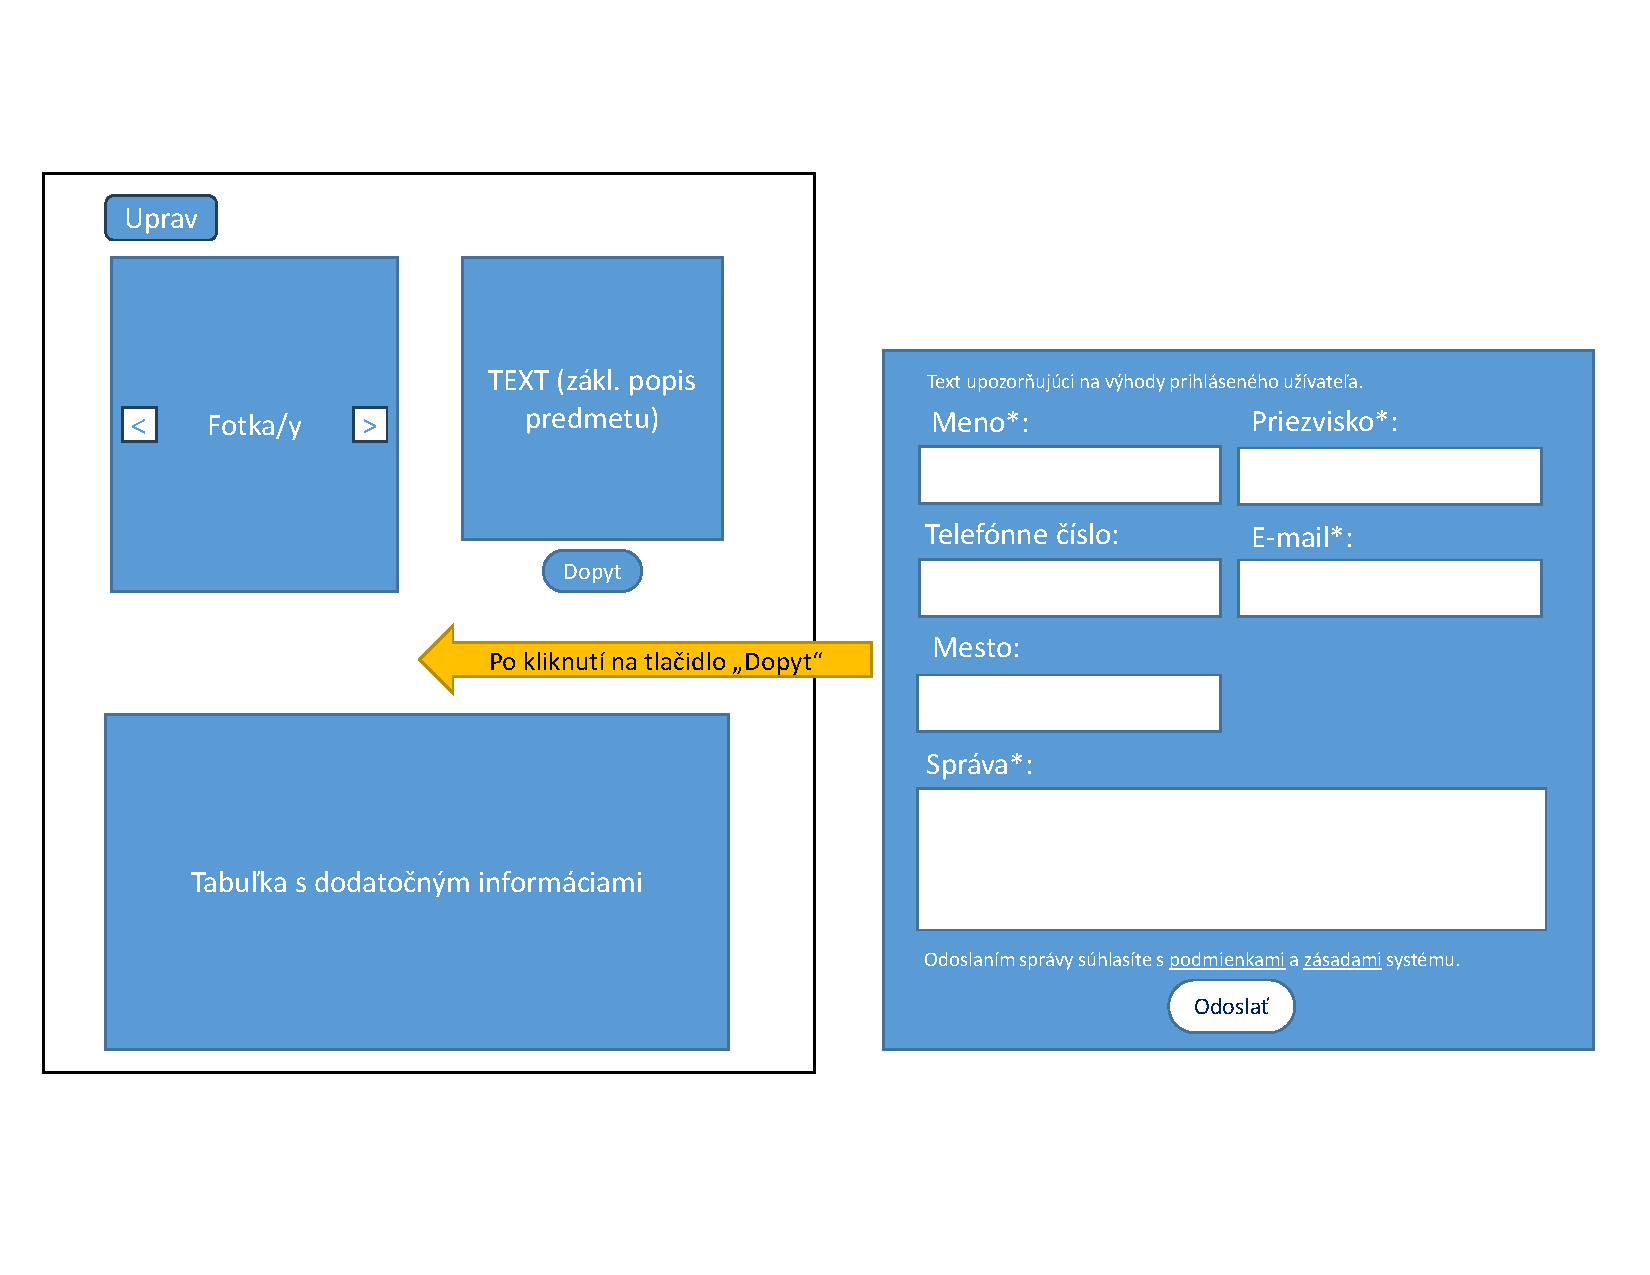
\includegraphics[width=140mm]{../img/UI concept/detail}
\caption{Detail bagra/prídavného zariadenia.}
\label{detail}
\end{figure}

V~tejto časti by sa mali nachádzať fotky predmetu (klikaním na~tlačidlá šipiek vpravo, vľavo by sa malo dať prechádzať medzi fotkami predmetu). Ďalej by sa mal na~stránke nachádzať opis predmetu, a~takisto tabuľka s~dodatočnými informáciami~-- v~prípade bagra by to mali byť jeho vlastnosti (napr.~výška, šírka atď.), v~prípade prídavného zariadenia by to mali byť údaje o~tom, akej značky, kategórie, a~taktiež pre~akú kategóriu bagrov je dané prídavné zariadenie.

\textbf{Pohľad pre~zákazníkov:} V~tejto časti by sa malo nachádzať tlačidlo~,,Dopyt``. Po~kliknutí naň by sa mal zobraziť formulár, ktorým bude môcť užívateľ odoslať dopyt na~daný predmet. Po~opätovnom kliknutí na~tlačidlo by sa mal formulár zatvoriť.

\textbf{Pohľad pre~administrátorov:} V~hornej časti by sa malo nachádzať tlačidlo~,,Upraviť``. Po~kliknutí naň by mal byť administrátor presmerovaný na~formulár vybraného bagra (resp.~prídavného zariadenia). Pomocou formulára by mal byť administrátor schopný daný bager (resp.~prídavné zariadenie) upravovať.

\subsection{Dopyt}
\label{dopyt}

\textbf{Pohľad pre~zákazníkov:} V~predošlej časti textu bolo spomenuté, že v~detaile bagra alebo~prídavného zariadenia by sa malo nachádzať tlačidlo~,,Dopyt``, ktorým by si mal byť zákazník schopný zobraziť (a~opätovným kliknutím schovať) formulár pre~odosielanie dopytu na~daný predmet. Pre~lepšiu predstavu formulára viď~pravú časť obrázka~\ref{detail}.

Formulár by mal obsahovať:
\begin{itemize}
\item \textit{Pre~neprihláseného zákazníka:}
Povinné polia meno, priezvisko, email, sprá\-va, a~takisto nepovinné polia telefón, mesto. Okrem polí by mal v~sebe formulár obsahovať správu upozorňujúcu na~to, že prihlásený užívateľ nemusí vypĺňať svoje osobné údaje, a takisto upozornenie, že odoslaním správy súhlasí s~podmienkami a~zásadami aplikácie. Upozornenie by malo zároveň fungovať ako odkaz do~časti aplikácie s podmienkami používania, a~tiež ako odkaz do~časti so~zásadami ochrany osobných údajov (obe časti boli spomenuté v~podkap.~\ref{gdpr}).
\item \textit{Pre~prihláseného zákazníka:}
Povinné pole správa.
\end{itemize}
Povinné polia by mali byť označené hviezdičkou.

Ďalej by mal formulár obsahovať tlačidlo~,,Odoslať``, ktoré by malo zákazníkovi umožniť odoslanie dopytu. Ak by boli po~kliknutí na~tlačidlo~,,Odoslať`` povinné údaje nevyplnené, tak by mala na~to aplikácia užívateľa upozorniť chybovými správami pri~jednotlivých poliach.

\subsection{Vytvorenie nového a úprava existujúceho bagra}
\label{vytvorenie noveho a uprava existujuceho bagra}

\textbf{Pohľad pre~administrátorov:} Kliknutím na~odkaz~,,Pridať nový bager``, ktorý by sa mal nachádzať v~časti s~vylistovanými (novými) bagrami, by mal byť administrátor presmerovaný do~časti aplikácie, kde bude môcť vytvoriť nový bager. Pre~lepšiu predstavu tejto časti aplikácie viď~obr.~\ref{excavator form}.

\begin{figure}[H]\centering
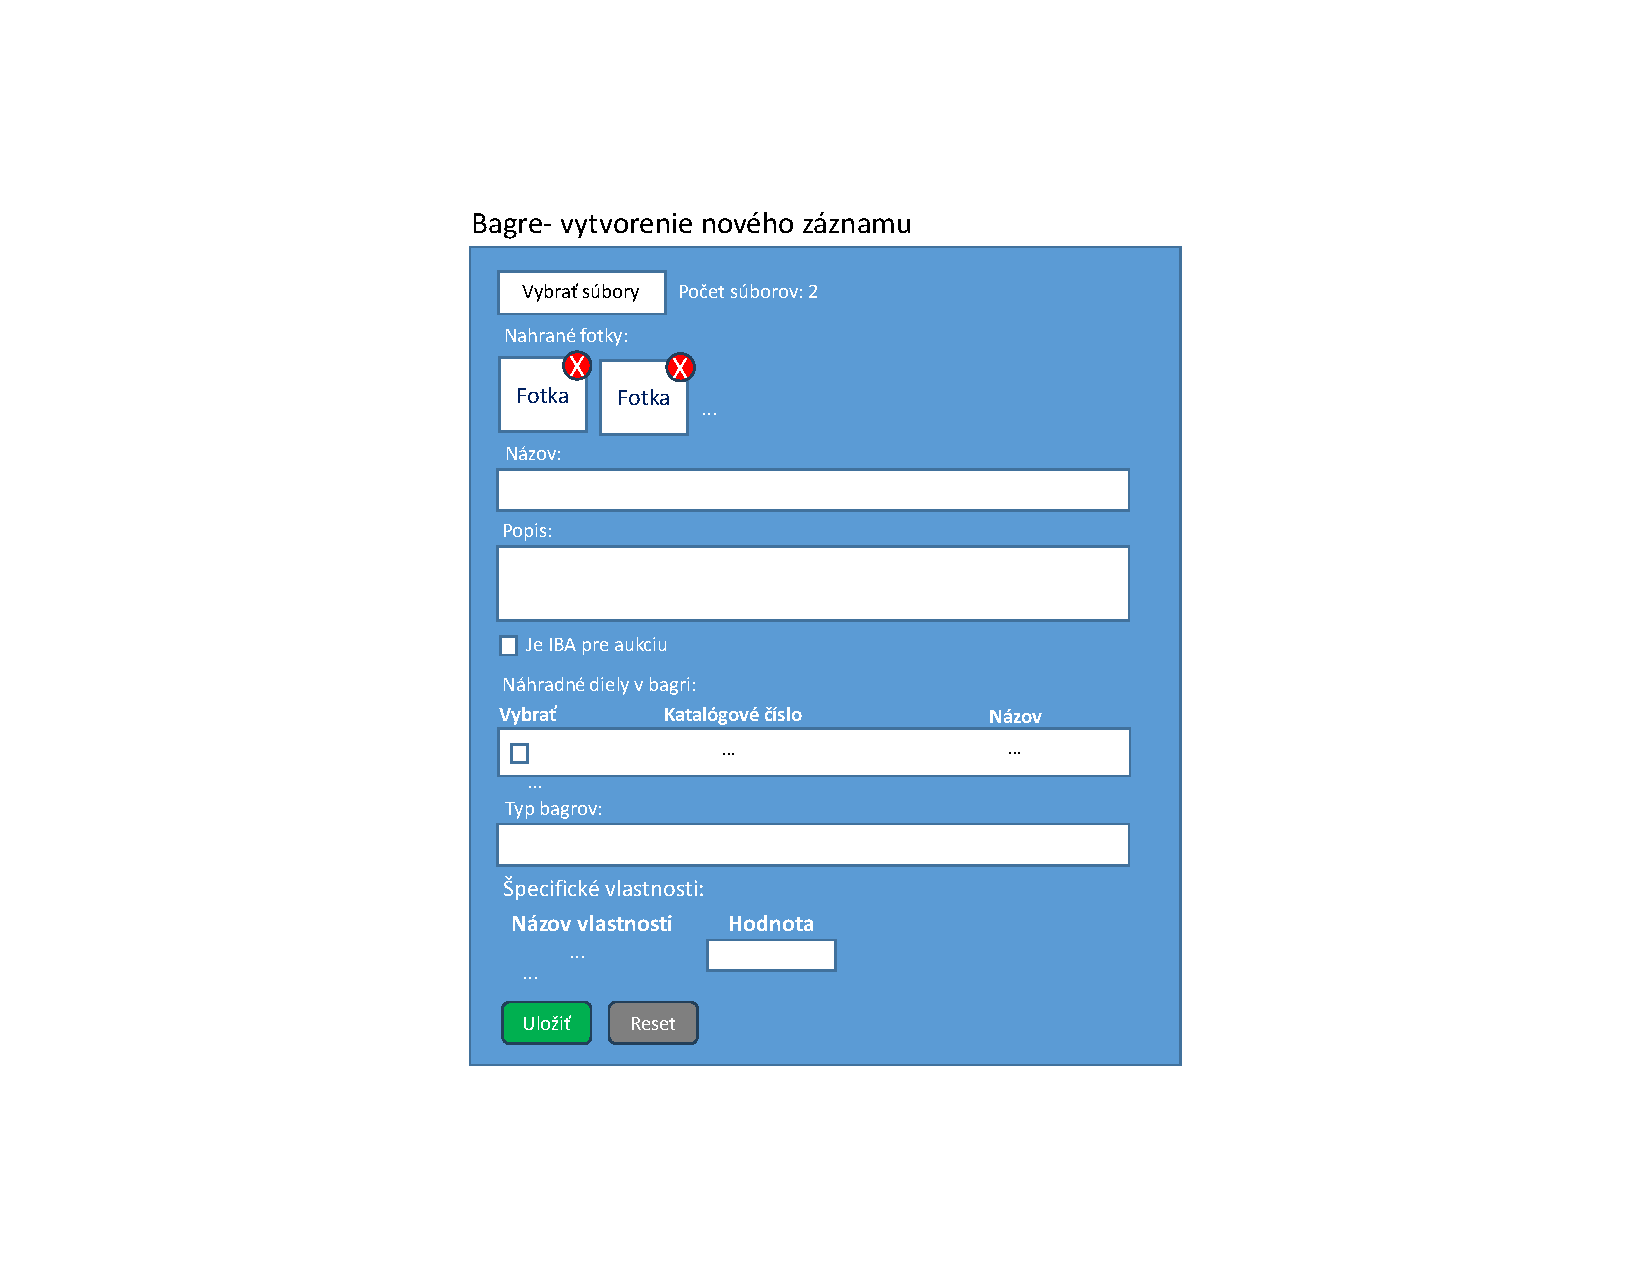
\includegraphics[width=140mm]{../img/UI concept/excavator form}
\caption{Časť aplikácie pre~vytvorenie bagra.}
\label{excavator form}
\end{figure}

Podobne kliknutím na~tlačidlo~,,Upraviť``, ktoré by sa malo nachádzať v~časti s~detailom bagra, by mal byť administrátor presmerovaný do~časti aplikácie, kde by mal byť schopný upravovať daný bager. V~následujúcom opise uvidíme, že obe časti aplikácie (časť pre~vytváranie a~časť pre~upravovanie bagra) sú si veľmi podobné.

Obidve časti by mali obsahovať formulár umožňujúci vloženie viacerých fotiek, názvu bagra, zadanie jeho popisu, uvedenie, či je stroj určený iba pre~aukciu, tiež by mal byť administrátor schopný vybrať, ktoré náhradné diely patria do~daného bagra, a~takisto vybrať z~možností typov bagrov. Podľa vybraného typu bagra by sa mali zobraziť vlastnosti ním určené a~administrátor by mal byť schopný vyplniť ich hodnoty. Fotky, názov bagra a~jeho typ patria medzi povinné údaje.

Navyše po~vložení by sa mali fotky a~ich počet zobraziť vo~formulári. V~pravom hornom rohu každej zobrazenej fotky by sa malo nachádzať tlačidlo~,,X``, ktorým by mal byť administrátor schopný fotku odstrániť.

Formulár by taktiež mal obsahovať tlačidlá ,,Uložiť`` (na~uloženie bagra) a~,,Reset`` (na~vyprázdenie formulára). Ak by boli po~kliknutí na~tlačidlo~,,Uložiť`` povinné údaje nevyplnené, tak by mal na~to systém administrátora upozorniť prostrednictvom chybových správ pri~jednotlivých poliach.

Navyše nad~formulárom by mal byť v~prípade vytvárania nového bagra nadpis ,,Bagre~-- vytvorenie nového záznamu``. V~prípade úpravy existujúceho bagra by tam mal byť nadpis ,,Bagre~-- úprava existujúceho záznamu``.

\subsection{Úprava bagrov, ktoré nie sú v ponuke (nových) bagrov}

\textbf{Pohľad pre~administrátorov:} V~predošlom texte bolo napísané, že administrátor by sa mal byť schopný dostať cez~karty hlavných ponúk k~ponuke (nových) bagrov a~cez nich k~detailu bagra, kde môže kliknutím na~tlačidlo~,,Upraviť`` upravovať daný bager. Ale ak by administrátor vytvoril bager typu, pre~ktorý neexistuje hlavná ponuka alebo~bager určený iba pre~aukciu, tak by sa bager nezobrazoval medzi ponukou (nových) bagrov.

Preto by mala byť pre~takéto bagre (a~tiež pre~položky s~podobným problémom) vyhradená osobitná časť aplikácie, kde ich bude môcť administrátor spravovať (t.~j.~vytvárať, upravovať a~mazať). Viac o~tejto časti aplikácie v~podkapitole~\ref{splnenie p5 p7 a sprava predmetov}.

\subsection{Vytvorenie nového a úprava existujúceho prídavného zariadenia}
\label{vytvorenie noveho a uprava existujuceho pridavného zariadenia}

\textbf{Pohľad pre~administrátorov:} Kliknutím na~odkaz~,,Pridať nové prídavné zariadenie``, ktorý by sa mal nachádzať v~časti s~vylistovanými prídavnými zariadeniami, by mal byť administrátor presmerovaný do~časti aplikácie, kde by mal byť schopný vytvoriť nové prídavné zariadenie. Pre~lepšiu predstavu tejto časti viď~obr.~\ref{additional equipment form}.

\begin{figure}[H]\centering
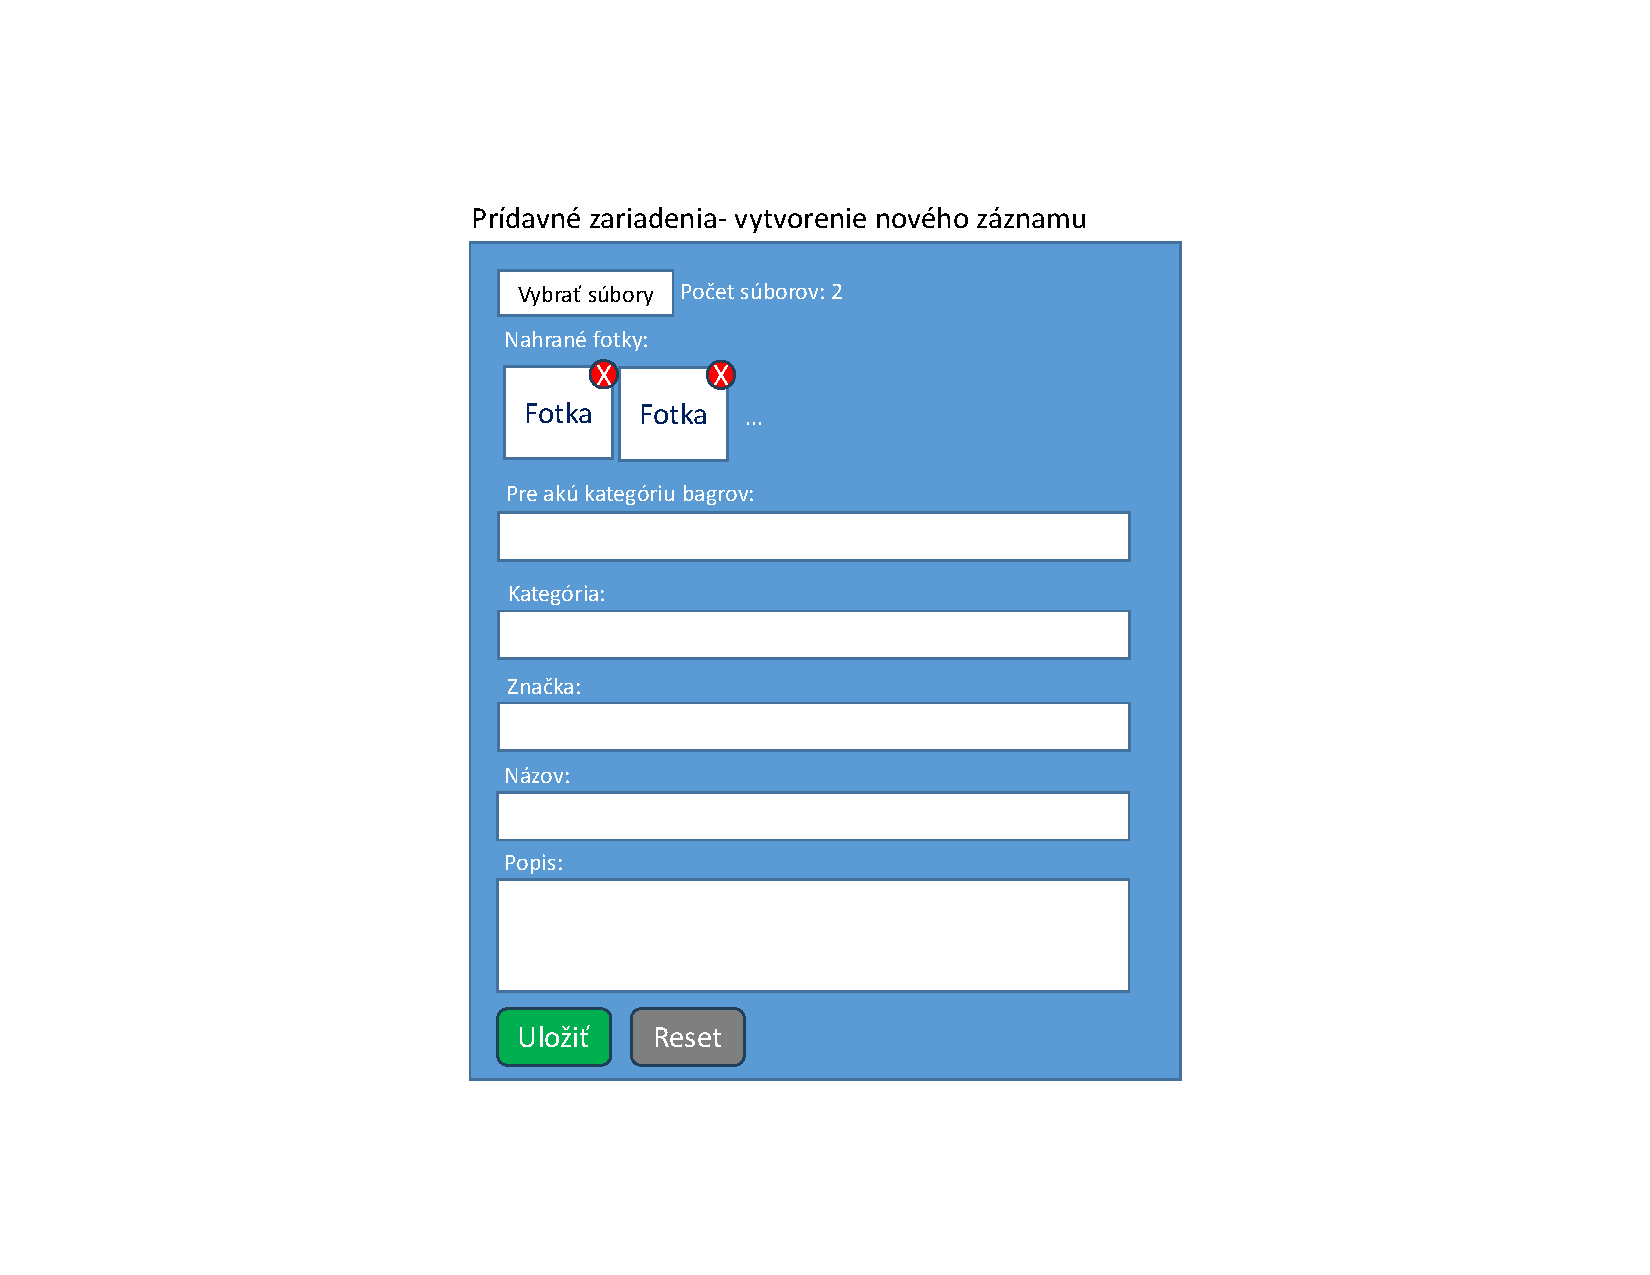
\includegraphics[width=140mm]{../img/UI concept/additional equipment form}
\caption{Časť aplikácie pre~vytvorenie prídavného zariadenia.}
\label{additional equipment form}
\end{figure}

Podobne kliknutím na~tlačidlo~,,Upraviť``, ktoré by sa malo nachádzať v~časti s~detailom prídavného zariadenia, by mal byť administrátor presmerovaný do~časti aplikácie, kde by mal byť schopný upravovať dané prídavné zariadenie. Ako uvidíme v~následujúcom opise, obe časti aplikácie (časť pre~vytváranie a~časť pre~upravovanie prídavného zariadenia) sú si veľmi podobné.

Obe časti by mali obsahovať formulár umožňujúci vloženie viacerých fotiek, vybranie kategórie bagrov (pre~ktoré je prídavné zariadenie určené), vybranie jeho kategórie, vybranie značky, a~takisto zadanie názvu a~popisu prídavného zariadenia. Okrem popisu sú všetky údaje povinné. Navyše po~vložení by sa mali fotky a~ich počet zobraziť vo~formulári. V~pravom hornom rohu každej zobrazenej fotky by sa malo nachádzať tlačidlo~,,X``, ktorým môže administrátor fotku odstrániť.

Formulár by mal taktiež obsahovať tlačidlá ,,Uložiť`` (na~uloženie prídavného zariadenia) a~,,Reset`` (na~vyprázdenie formulára). Ak by boli po~kliknutí na~tlačidlo~,,Uložiť`` povinné údaje nevyplnené, tak by mal na~to systém administrátora upozorniť prostrednictvom chybových správ pri~jednotlivých poliach.

Navyše nad~formulárom by mal byť v~prípade vytvárania nového bagra nadpis ,,Prídavné zariadenia~-- vytvorenie nového záznamu``. V~prípade úpravy existujúceho prídavného zariadenia by tam mal byť nadpis ,,Prídavné zariadenia~-- úprava existujúceho záznamu``.

\section{Splnenie P4}

V~tejto podkapitole si prejdeme časti aplikácie splňujúce požiadavku~P4, t.~j.~predstavenie aukčnej ponuky, časti umožňujúce administrátorovi vytvárať (a~upravovať) aukčné ponuky, a~takisto časti umožňujúce zákazníkom ponúkať sumy do~dražby. Pre~lepšie pochopenie prechádzania medzi jednotlivými časťami programu viď~obr.~\ref{p4 graph}.

\begin{figure}[H]\centering
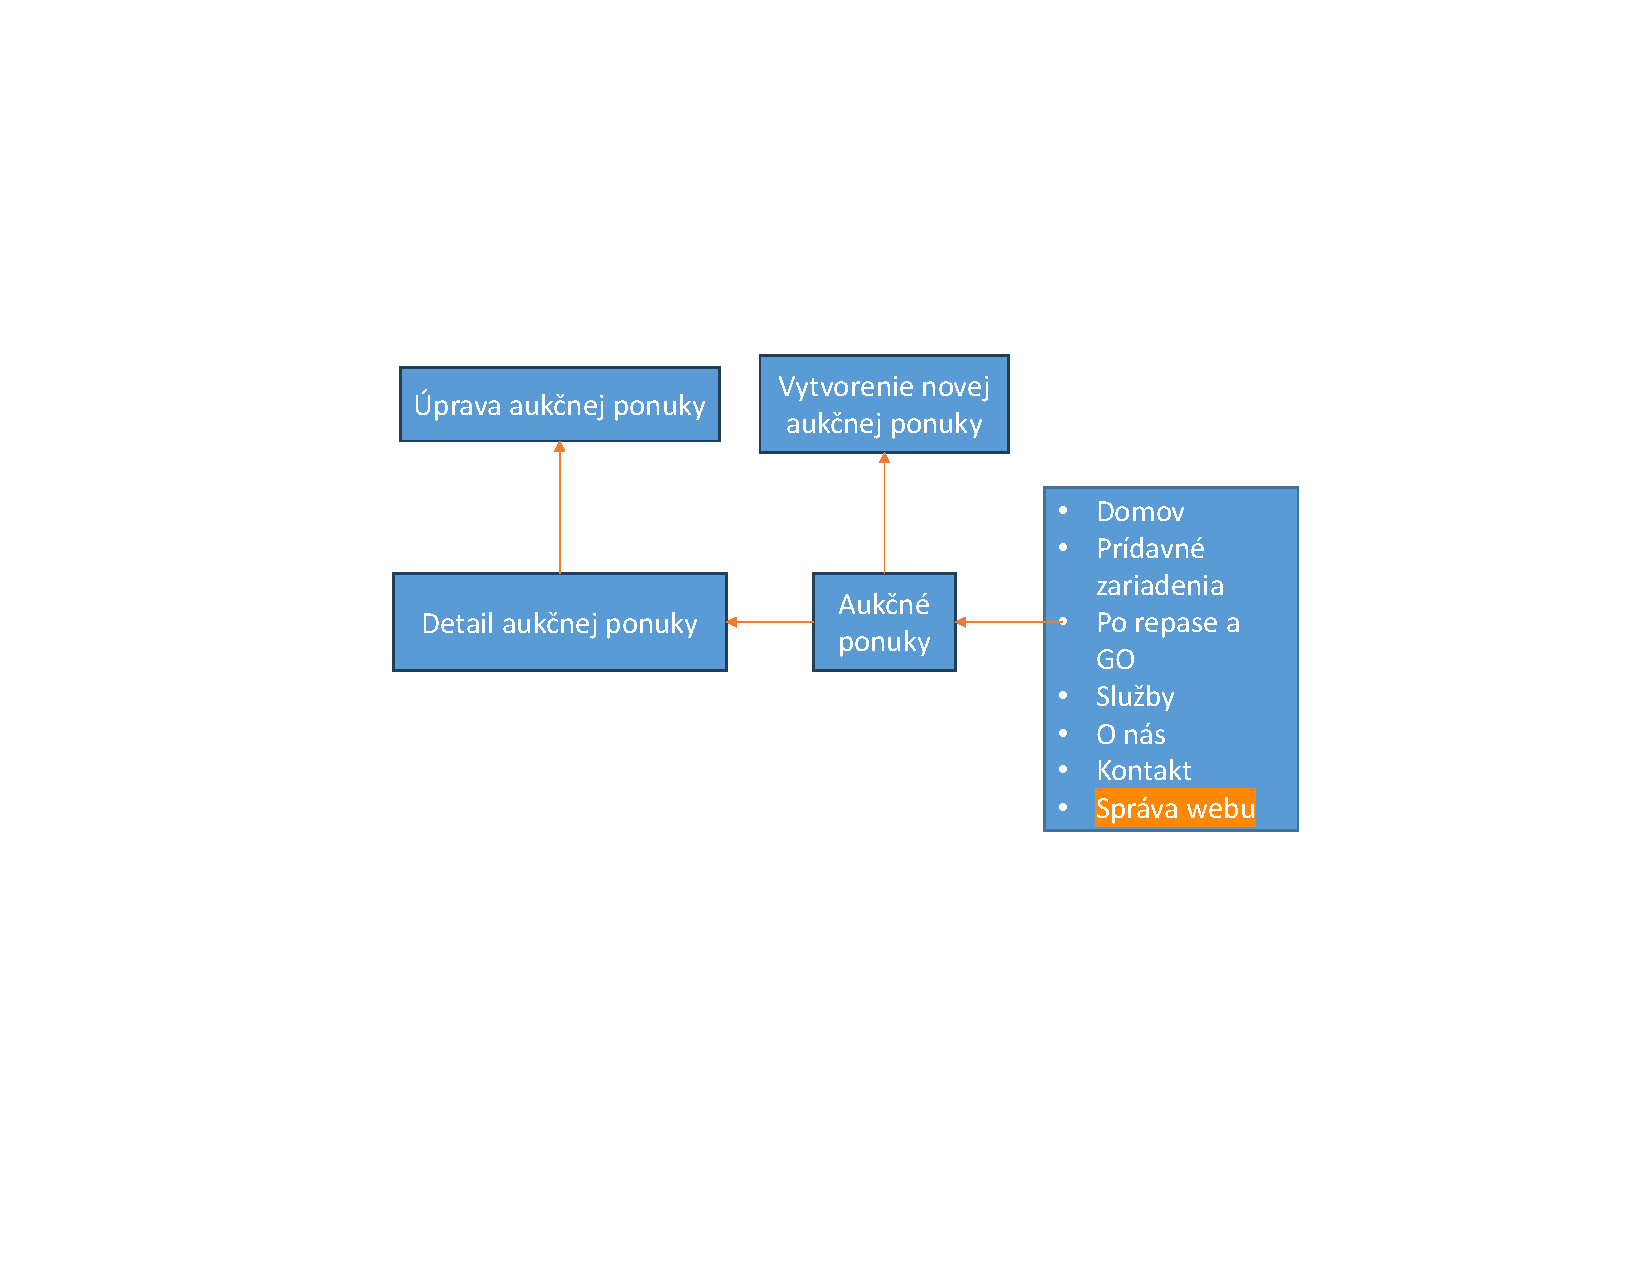
\includegraphics[width=140mm]{../img/UI concept/p4 graph}
\caption{Prechádzanie medzi časťami aplikácie spĺňajúcimi požiadavku P4.}
\label{p4 graph}
\end{figure}

\textbf{Spoločný pohľad:} Po~kliknutí na~odkaz~,,Po repase a~GO`` v~navigácii by mala byť užívateľovi zobrazená časť aplikácie s~vylistovanými kartami aukčnej ponuky~-- Aukčné ponuky (viď hranu 1 na~obr.~\ref{p4 graph}). Po~kliknutí na~nejakú z~kariet by sa mal užívateľovi zobraziť detail aukčnej ponuky (viď hranu 2 na~obr.~\ref{p4 graph}). 

\textbf{Pohľad pre~zákazníkov:} V časti aplikácie s detailom aukčnej ponuky by sa malo zobrazovať tlačidlo~\uv{Mám záujem!}, pomocou ktorého by si mal byť zákazník schopný zobraziť (a~opätovným kliknutím schovať) formulár pre~ponúknutie sumy do~dražby. Vo formulári by sa mal tiež nachádzať odkaz do~časti aplikácie s~podmienkami používania (viď hranu 5 na obr. \ref{p4 graph}), a takisto aj odkaz do časti so zásadami ochrany užívateľských údajov (viď hranu 6 na obr. \ref{p2 p3 graph}).

\textbf{Pohľad pre~administrátorov:} Nad~vylistovanými kartami by sa mal zobrazovať odkaz~,,Pridať novú aukčnú ponuku``. Pomocou tohto odkazu by sa mal byť administrátor schopný dostať do~časti aplikácie s~prázdnym formulárom pre~vytvorenie novej aukčnej ponuky (viď hranu 3 na~obr.~\ref{p4 graph}).

V~hornej časti detailu aukčnej ponuky by sa malo zobrazovať tlačidlo~,,Upraviť``. Pomocou tohto tlačidla by sa mal byť administrátor schopný dostať do~časti aplikácie, kde by mal byť schopný danú ponuku upravovať (viď hranu 4 na~obr.~\ref{p4 graph}).

\subsection{Aukčné ponuky}
\label{aukcne ponuky}

Kliknutím na~odkaz~,,Po repase a~GO`` v~navigácii by mal byť užívateľ presmerovaný do~časti aplikácie s~vylistovanými kartami aukčných ponúk. Pre~lepšiu predstavu viď~obr.~\ref{auction offer cards}.

\begin{figure}[H]\centering
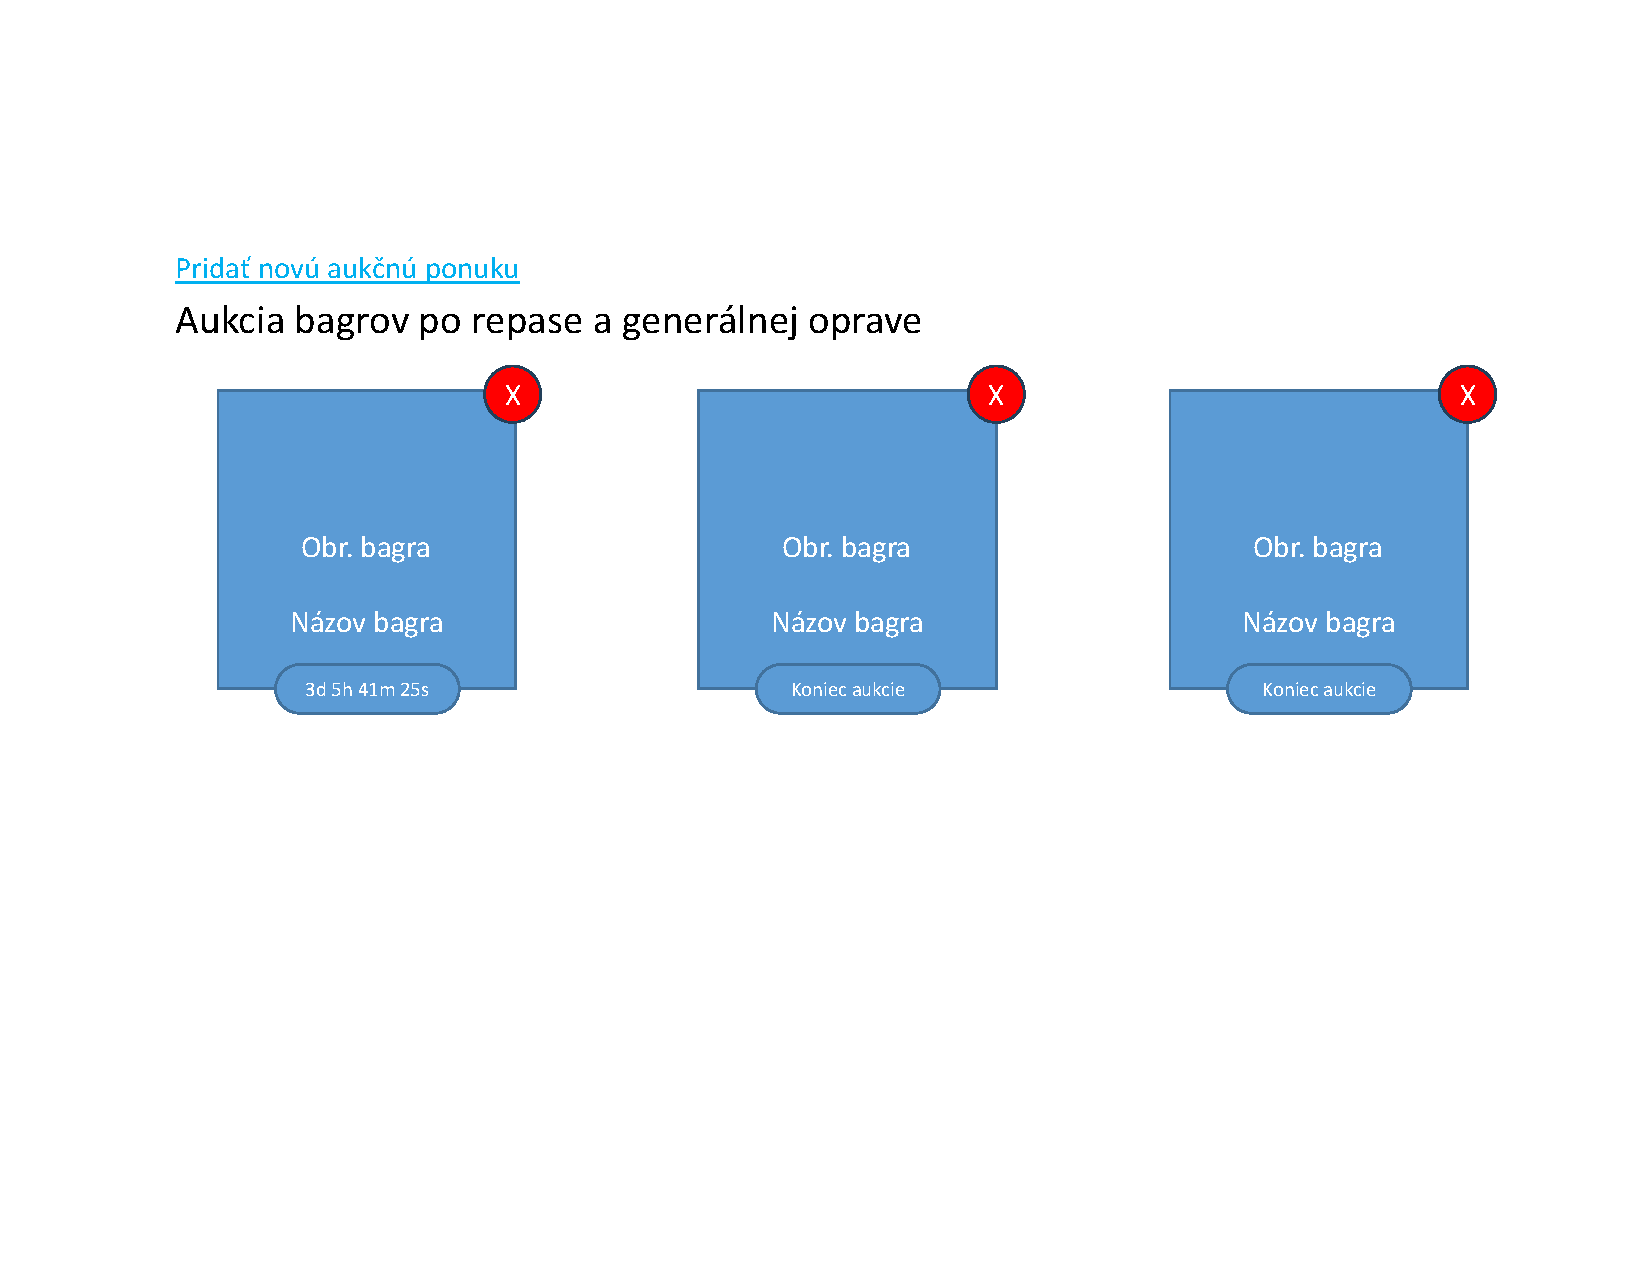
\includegraphics[width=140mm]{../img/UI concept/auction offer cards}
\caption{Aukčné ponuky.}
\label{auction offer cards}
\end{figure}

\textbf{Spoločný pohľad:} Karta aukčnej ponuky by mala obsahovať obrázok a~názov draženého bagra. V~spodnej časti by sa mal nachádzať odpočet do~konca dražby. Po~kliknutí na~nejakú z~kariet by mal byť užívateľ presmerovaný na~detail vybranej aukčnej ponuky. Nad~kartami by sa mal nachádzať nadpis~,,Aukcia bagrov po~repase a~generálnej oprave``.

\textbf{Pohľad pre~administrátorov:} V~pravej hornej časti karty aukčnej ponuky by malo byť tlačidlo~,,X``, ktorým by mal byť administrátor schopný ponuku vymazať. Po~kliknutí naň by sa malo zobraziť modálne potvrdzovacie okno s~nadpisom~,,Vymazať aukčnú ponuku natrvalo`` a~textom \uv{Naozaj chcete túto aukčnú ponuku vymazať natrvalo?}.

Vo~vrchnej časti s vylistovanými kartami aukčnej ponuky by sa mal nachádzať odkaz~,,Pridať novú aukčnú ponuku``. Po~kliknutí na odkaz by mal byť administrátor presmerovaný do~časti aplikácie, kde by mohol vytvoriť novú aukčnú ponuku.

\subsection{Detail aukčnej ponuky}
\label{detail aukcnej ponuky}

Po~kliknutí na~nejakú z~kariet aukčnej ponuky by mal byť užívateľ presmerovaný do~časti detailu aukčnej ponuky. Pre~lepšiu predstavu viď~obr.~\ref{auction offer detail}.

\begin{figure}[H]\centering
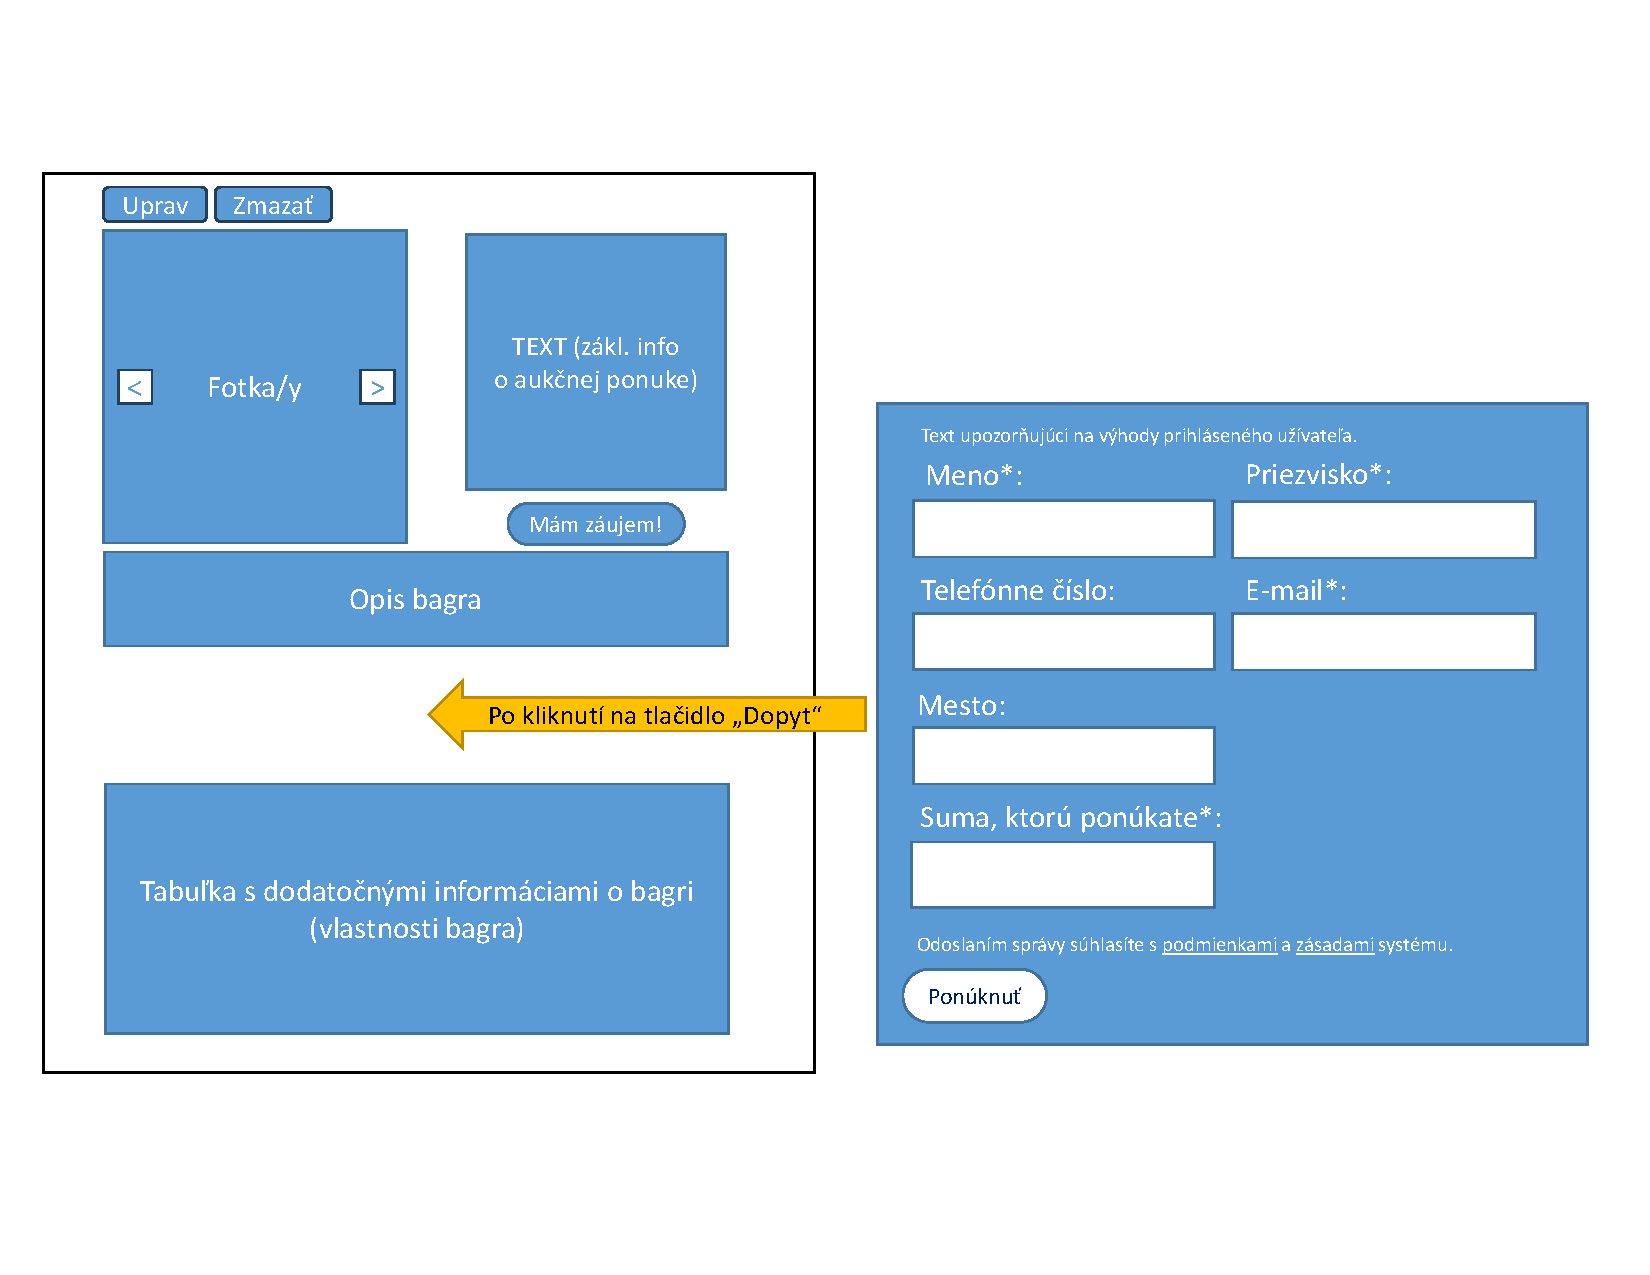
\includegraphics[width=140mm]{../img/UI concept/auction offer detail}
\caption{Detail aukčnej ponuky.}
\label{auction offer detail}
\end{figure}

\textbf{Spoločný pohľad:} V~tejto časti by sa mali nachádzať fotky draženého bagra (klikaním na~tlačidlá šipiek vpravo, vľavo by sa malo dať prechádzať medzi fotkami predmetu). Ďalej by sa mali v~tejto časti aplikácie nachádzať základné informácie o~aukčnej ponuke bagra (napr.~aký je bager starý, čo na~ňom bolo opravované atď.), okrem toho by mal byť v~tejto časti aj všeobecný popis bagra (všeobecné informácie o~bagri, ktoré platia nezávislé od~toho, že bol opravovaný), ďalej by sa v~tejto časti mala nachádzať tabuľka s~vlastnosťami bagra (napr.~výška, šírka atď.).

\textbf{Pohľad pre~zákazníkov:} Okrem toho by sa malo v~tejto časti ešte nachádzať tlačidlo~~\uv{Mám záujem!}. Po~kliknutí naň by sa mal zobraziť formulár, ktorým by mal byť užívateľ schopný ponúknuť sumu do~dražby. Po~opätovnom kliknutí na~tlačidlo sa má formulár zatvoriť.

\textbf{Pohľad pre~administrátorov:} V~hornej časti detailu aukčnej ponuky by sa malo nachádzať tlačidlo~,,Upraviť``. Po~kliknutí naň by mal byť administrátor presmerovaný na~formulár danej aukčnej ponuky, ktorým by ju mal byť schopný upravovať. Okrem tlačidla~,,Upraviť`` by sa v~hornej časti malo nachádzať aj tlačidlo~,,Zmazať``, ktorým by mal byť schopný danú aukčnú ponuku zmazať. Po~kliknutí na~tlačidlo~\uv{Zmazať} by sa malo zobraziť modálne potvrdzovacie okno s~nadpisom~,,Vymazať`` a~textom \uv{Naozaj chcete vymazať túto aukčnú ponuku?}.

\subsection{Ponúkanie sumy do~dražby}
\label{ponukanie sumy do drazby}

\textbf{Pohľad pre~zákazníkov:} V~predošlej časti textu bolo spomenuté, že v~detaile bagra alebo~prídavného zariadenia by sa malo nachádzať tlačidlo~\uv{Mám záujem!}, ktorým by si mal byť zákazník (nie administrátor) schopný zobraziť (a~opätovným kliknutím schovať) formulár pre~ponúknutie sumy do~dražby daného bagra. Pre~lepšiu predstavu formulára viď~pravú časť obrázka~\ref{auction offer detail}.

Formulár by mal obsahovať:
\begin{itemize}
\item \textit{Pre neprihláseného zákazníka:}
Povinné polia meno, priezvisko, email, pole pre~ponúkanú sumu, a~takisto nepovinné polia telefón, mesto. Okrem polí by mal v~sebe formulár obsahovať aj správu upozorňujúcu na~to, že prihlásený užívateľ nemusí vypĺňať svoje osobné údaje, a takisto aj upozornenie, že s~odoslaním správy súhlasí s~podmienkami a~zásadami aplikácie. Upozornenie by malo zároveň fungovať ako odkaz do~časti aplikácie s podmienkami používania, a~tiež ako odkaz do~časti so~zásadami ochrany osobných údajov (obe časti boli spomenuté v~podkap.~\ref{gdpr}).
\item \textit{Pre prihláseného zákazníka:}
Povinné pole pre~ponúkanú sumu.
\end{itemize}
Povinné polia by mali byť označené hviezdičkou. Navyše má platiť, že prvá zákazníkom ponúknutá suma môže byť rovná počiatočnej sume, ale nasledujúce ponúkané sumy musia mať medzi sebou rozdiel aspoň 100~eur.

Ďalej by mal formulár obsahovať tlačidlo~,,Ponúknuť``, ktoré by malo zákazníkovi umožniť ponúknutie sumy do~dražby daného bagra. Ak by boli po~kliknutí na~tlačidlo~,,Ponúknuť`` povinné údaje nevyplnené~alebo ak by boli ich hodnoty neplatné, tak by mala na~to aplikácia užívateľa upozorniť chybovými správami pri~jednotlivých poliach.

\subsection{Vytvorenie novej a úprava existujúcej aukčnej ponuky}
\label{vytvorenie novej a uprava existujucej aukcnej ponuky}

\textbf{Pohľad pre~administrátorov:} Kliknutím na~odkaz~,,Pridať novú aukčnú ponuku``, ktorý by sa mal nachádzať v~časti s~vylistovanými aukčnými ponukami, by mal byť administrátor presmerovaný do~časti aplikácie, kde by mal byť schopný vytvoriť novú aukčnú ponuku. Pre~lepšiu predstavu tejto časti aplikácie viď~obr.~\ref{auction offer form}.

\begin{figure}[H]\centering
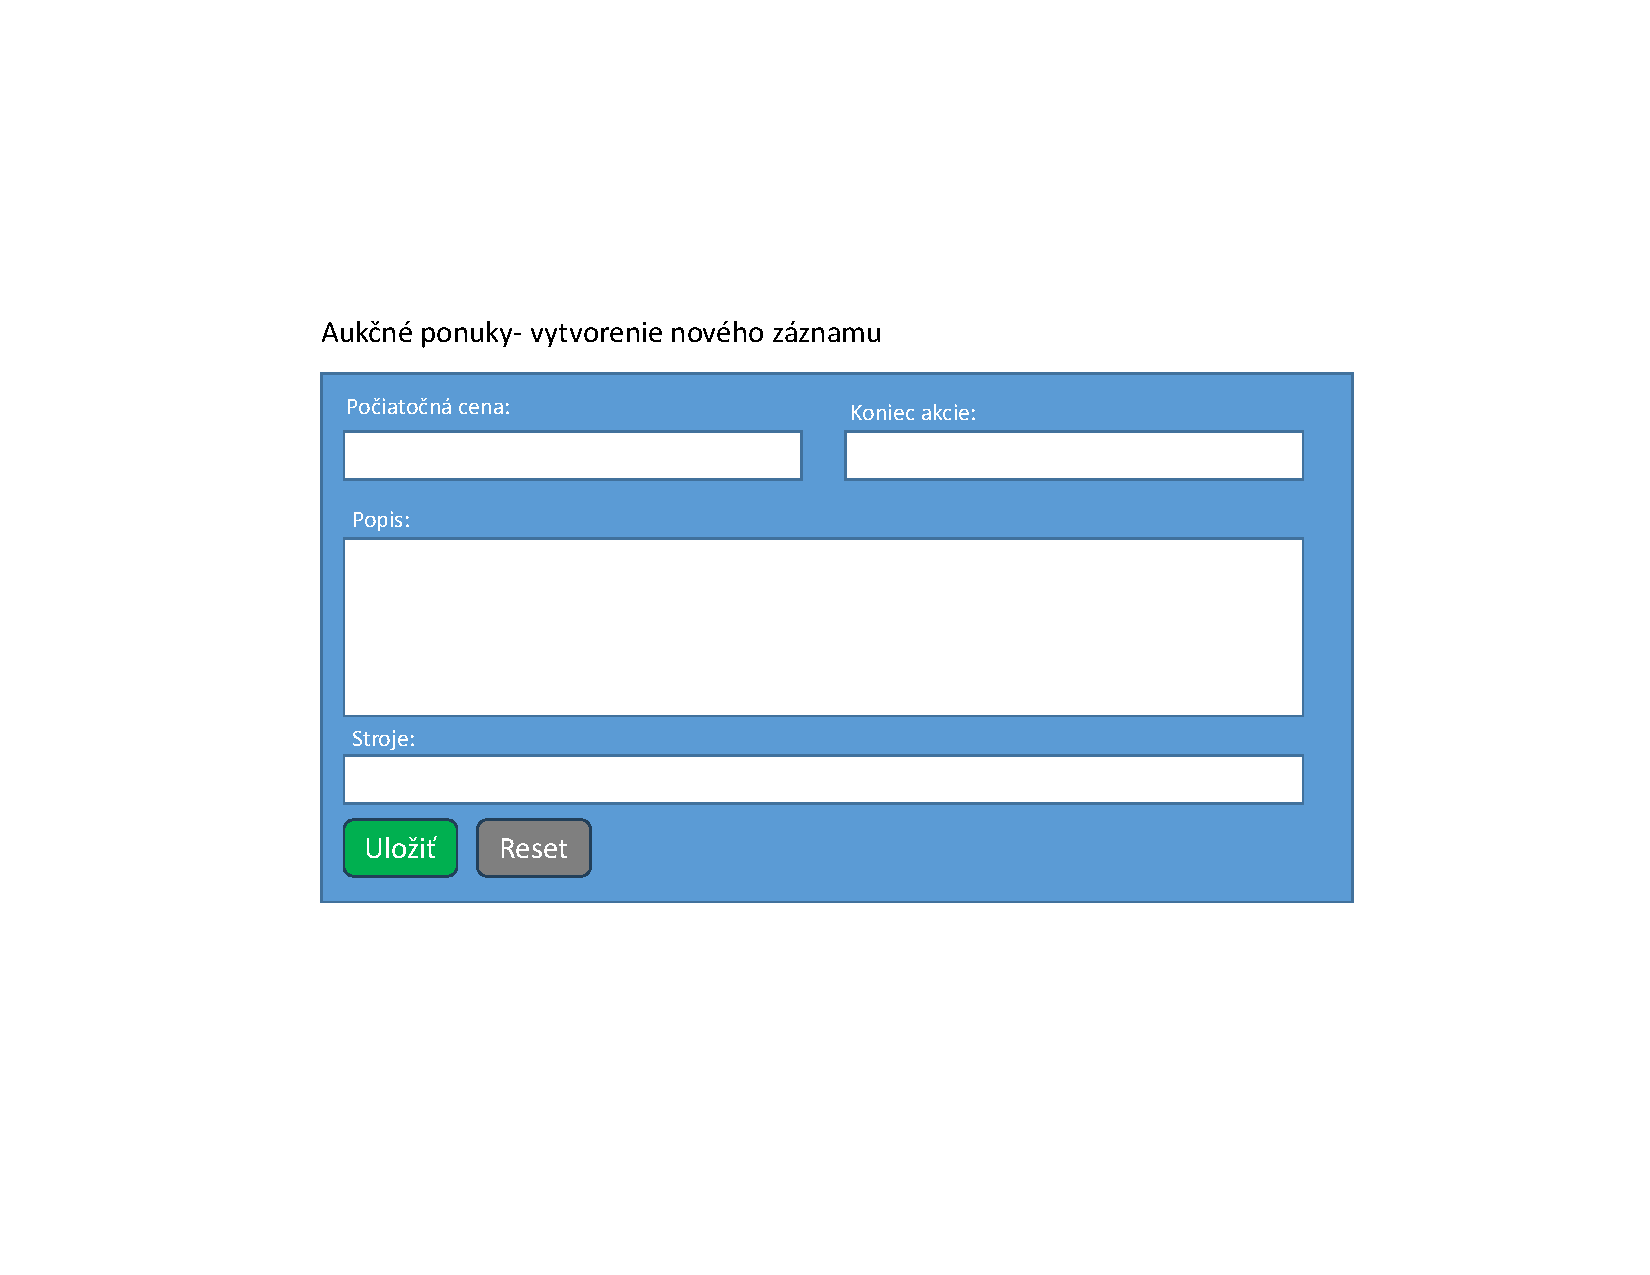
\includegraphics[width=140mm]{../img/UI concept/auction offer form}
\caption{Časť aplikácie pre~vytvorenie aukčnej ponuky.}
\label{auction offer form}
\end{figure}

Podobne kliknutím na~tlačidlo~,,Upraviť``, ktoré by sa malo nachádzať v~časti s~detailom aukčnej ponuky, by mal byť administrátor presmerovaný do~časti aplikácie, kde bude môcť danú aukčnú ponuku upravovať. Ako uvidíme v~následujúcom opise, obe časti aplikácie (časť pre~vytváranie a~časť pre~upravovanie aukčnej ponuky) sú si veľmi podobné.

Časť aplikácie pre~vytváranie novej aukčnej ponuky, ale takisto aj časť pre~u\-pra\-vo\-va\-nie existujúcej aukčnej ponuky, by mali obsahovať formulár umožňujúci vloženie počiatočnej (vyvolávacej) ceny draženého bagra, dátumu konca dražby, popisu (napr.~aké časti boli v~bagri opravované), a~takisto by mal formulár obsahovať možnosť výberu bagra do~dražby. Údaj o~bagri je povinný, dátum konca dražby nesmie obsahovať dátum v~minulosti a~počiatočná cena nesmie byť záporná.

Formulár by mal taktiež obsahovať tlačidlo~,,Reset`` na~vyprázdenie formulára. Okrem tlačidla~,,Reset`` by mal formulár obsahovať aj tlačidlo ,,Uložiť`` (na~uloženie aukčnej ponuky) ak sa vytvára nová aukčná ponuka alebo upravuje existujúca aukčná ponuka, ktorá je ešte stále aktívna (t.~j.~stále prebieha dražba). V~prípade, že by administrátor upravoval existujúcu aukčnú ponuku, ktorá už nie je aktívna, pretože stroj bol vydražený, tak by sa malo zobraziť tlačidlo~,,Uložiť a~spustiť odznova``. Toto správanie je vyžadované preto, lebo ak by výherca dražby z~nejakého dôvodu nesúhlasil s~prevzatím bagra, administrátor by mohol kliknutím na~tlačidlo~,,Uložiť a~spustiť odznova`` celú dražbu odštartovať odznova (teda ako novo vytvorenú, bez účastníkov a~ich ponúknutých súm). Ak by boli pri ukladaní povinné údaje nevyplnené~alebo by boli ich hodnoty neplatné, tak by mal na~to systém administrátora upozorniť prostrednictvom chybových správ pri~jednotlivých poliach.

Navyše nad~formulárom by mal byť v~prípade vytvárania novej aukčnej ponuky nadpis ,,Aukčné ponuky~-- vytvorenie nového záznamu``. V~prípade úpravy existujúcej aukčnej ponuky by mal byť nadpis ,,Aukčné ponuky~-- úprava existujúceho záznamu``.

\section{Splnenie P8}
\label{splnenie p8}

\textbf{Spoločný pohľad:} Po~kliknutí na~odkaz~,,Služby`` v~navigácii by mal byť užívateľ presmerovaný do~časti aplikácie, kde by mali byť opísané výkopové služby, ktoré firma ponúka. Pre~lepšiu predstavu prechodu medzi časťami aplikácie viď~obr.~\ref{p8 graph}. 

\begin{figure}[H]\centering
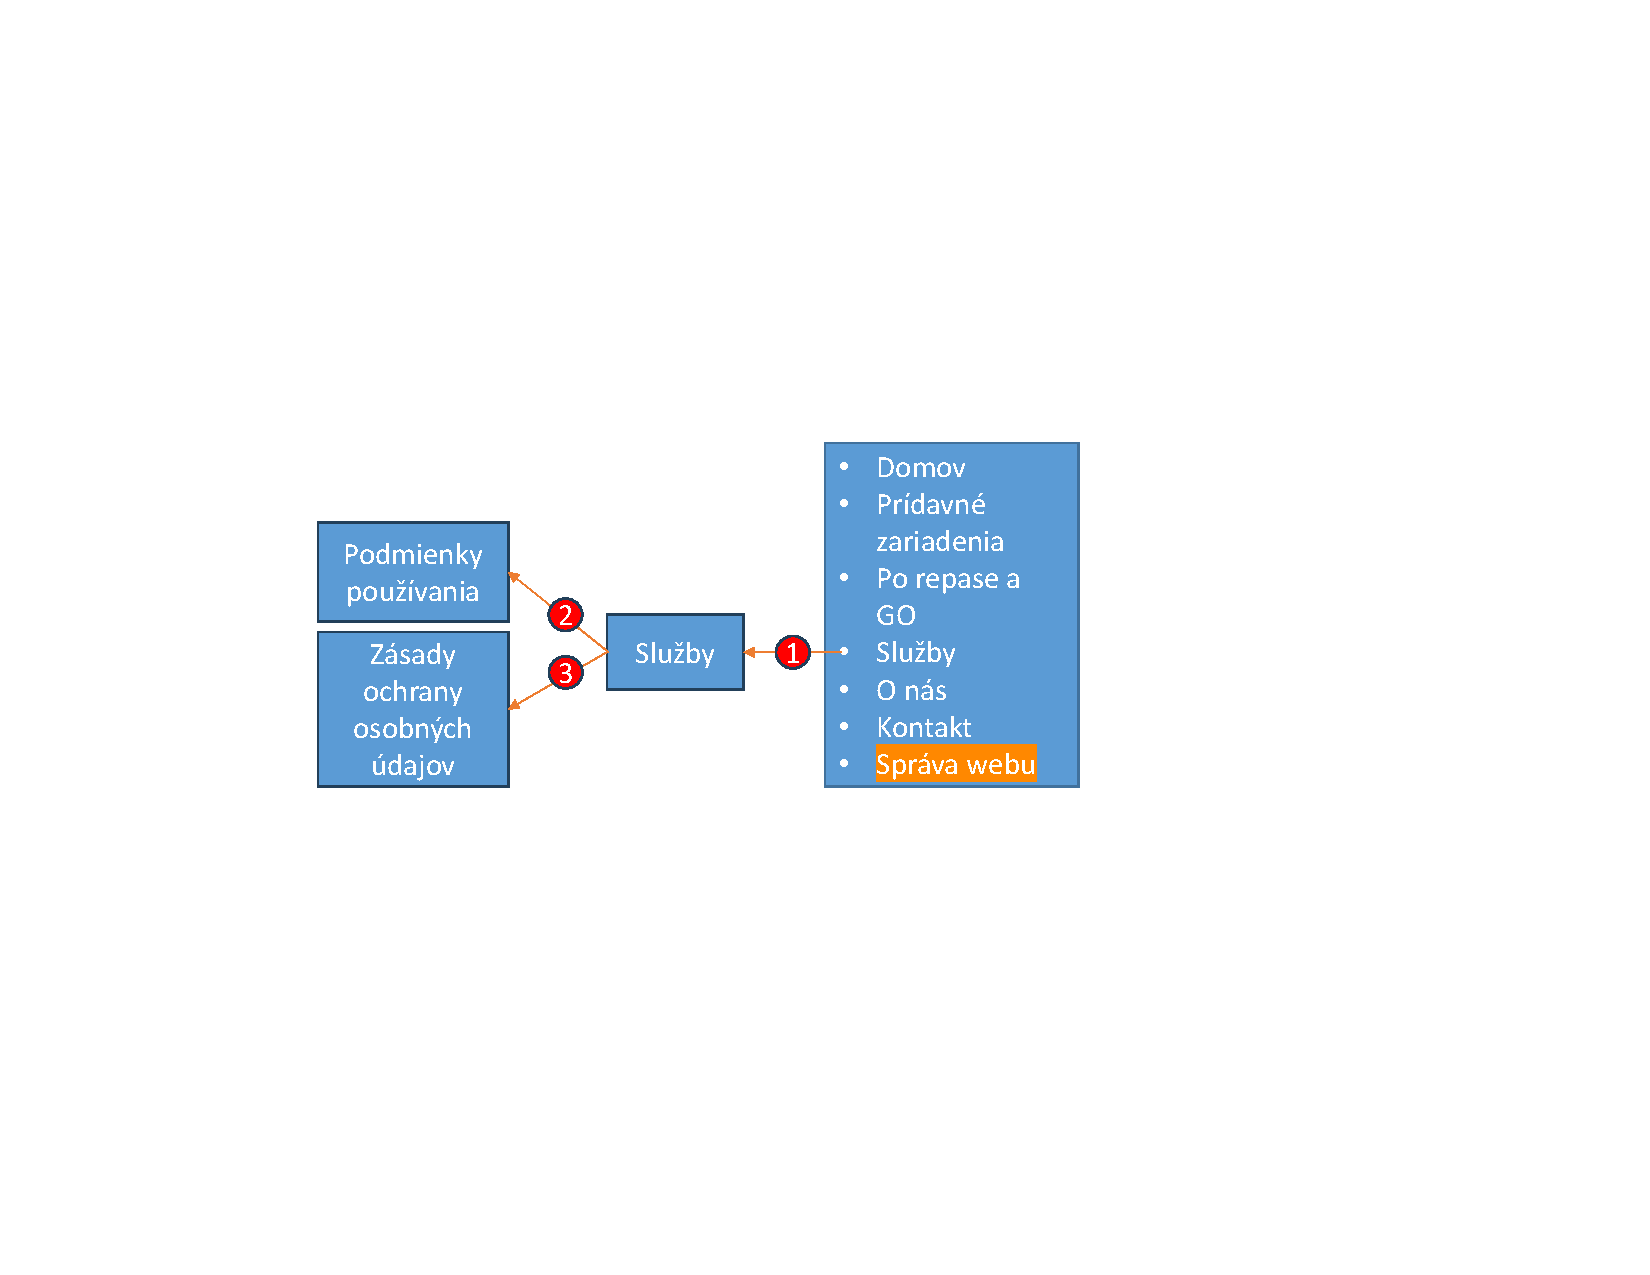
\includegraphics[width=140mm]{../img/UI concept/p8 graph}
\caption{Prechádzanie medzi časťami aplikácie spĺňajúcimi požiadavku~P8.}
\label{p8 graph}
\end{figure}

\textbf{Pohľad pre~zákazníkov:} V tejto časti aplikácie by sa malo nachádzať tlačidlo~\uv{Mám záujem o~službu!}. Kliknutím na~tlačidlo~\uv{Mám záujem o~službu!} by sa mal zobraziť formulár, ktorým by mal byť užívateľ schopný požiadať o~výkopovú službu. Pre~lepšiu predstavu formulára viď~pravú časť obr.~\ref{services}.

\begin{figure}[H]\centering
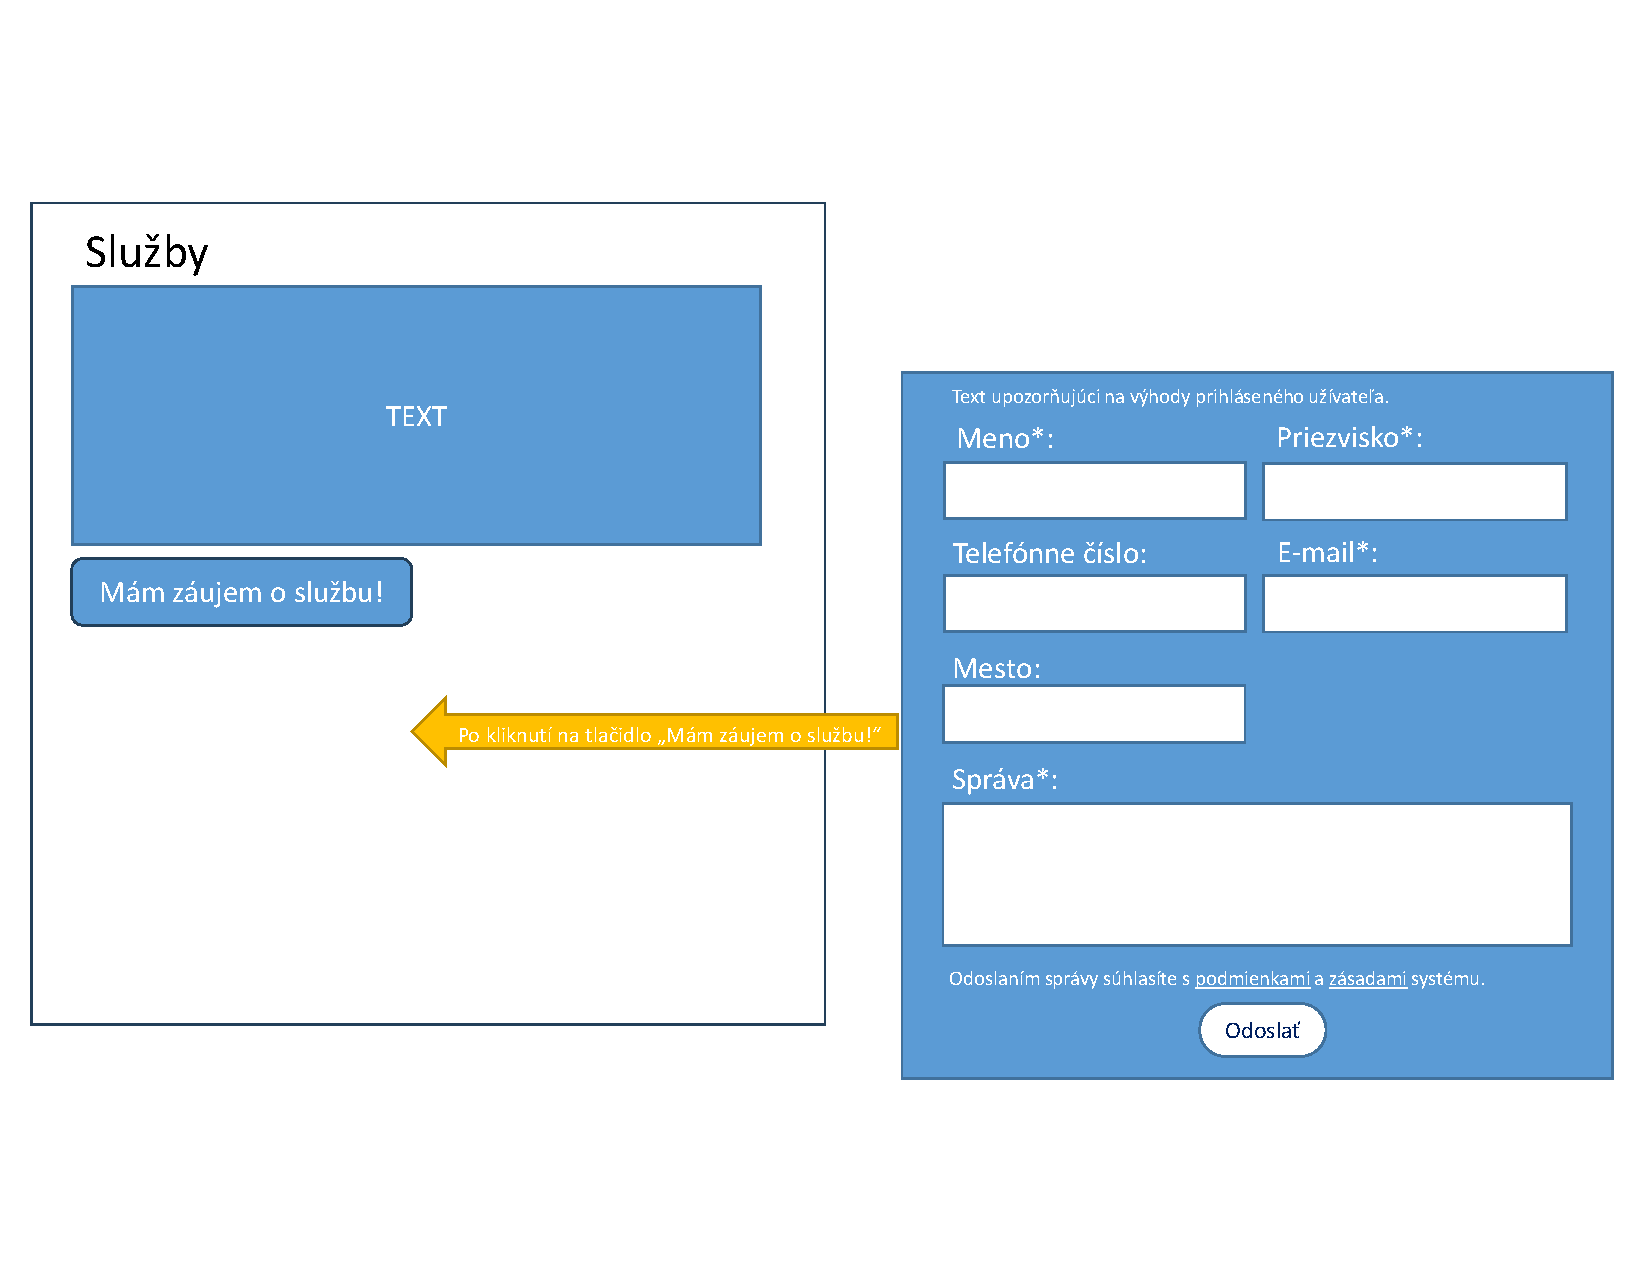
\includegraphics[width=140mm]{../img/UI concept/services}
\caption{Sekcia Služby.}
\label{services}
\end{figure}

Opätovným kliknutím na~tlačidlo by sa mal formulár schovať. Formulár by mal obsahovať:
\begin{itemize}
\item \textit{Pre neprihláseného zákazníka:}
Povinné polia meno, priezvisko, email, správa, a~takisto nepovinné polia telefón, mesto. Okrem polí by mal v~sebe formulár obsahovať správu upozorňujúcu na~to, že prihlásený užívateľ nemusí vypĺňať svoje osobné údaje, a takisto by mal formulár obsahovať upozornenie, že odoslaním správy súhlasí s~podmienkami a~zásadami aplikácie. Upozornenie by malo zároveň fungovať ako odkaz do~časti aplikácie s podmienkami používania (viď~hranu 2 na~obr.~\ref{p8 graph}), a~tiež ako odkaz do~časti so~zásadami ochrany osobných údajov (viď~hranu 3 na~obr.~\ref{p8 graph}), obe časti boli spomenuté v~podkap.~\ref{gdpr}.
\item \textit{Pre prihláseného zákazníka:}
Povinné pole správa.
\end{itemize}
Povinné polia by mali byť označené hviezdičkou.

Ďalej by mal formulár obsahovať tlačidlo~,,Odoslať``, ktoré by malo zákazníkovi umožniť odoslanie žiadosti o~službu. Ak by boli po~kliknutí na~tlačidlo~,,Odoslať`` povinné údaje nevyplnené, tak by na~to mala aplikácia užívateľa upozorniť chybovými správami pri~jednotlivých poliach.

\section{Splnenie P9}
\label{splnenie p9}

\textbf{Spoločný pohľad:} Po~kliknutí na~odkaz~,,O~nás`` v~navigácii by mal byť užívateľ presmerovaný do~časti aplikácie s informáciami o firme (viď~hranu~1 na~obr.\ref{p9 graph}). Pre~lepšiu predstavu sekcie~\uv{O~nás} viď~obr.~\ref{about}.

\begin{figure}[H]\centering
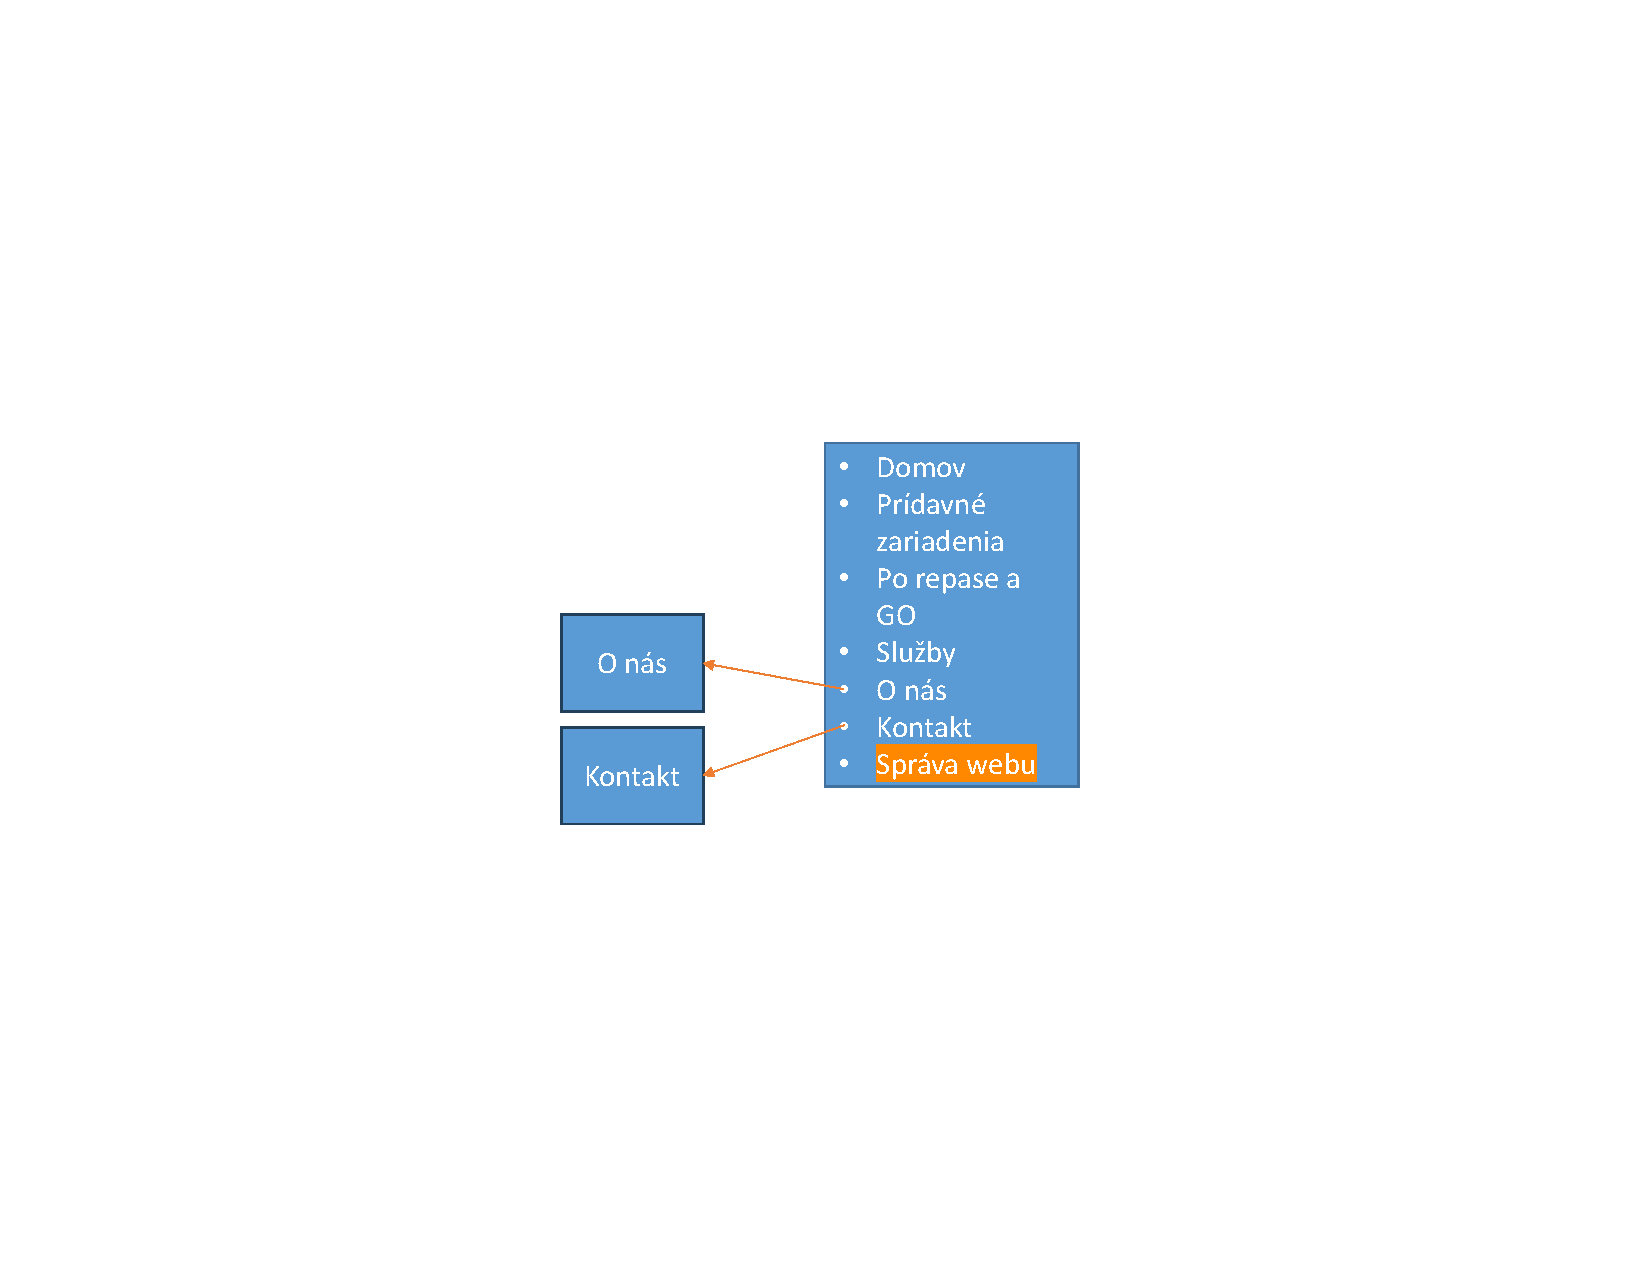
\includegraphics[width=140mm]{../img/UI concept/p9 graph}
\caption{Prechádzanie medzi časťami aplikácie spĺňajúcimi požiadavku~P9.}
\label{p9 graph}
\end{figure}

\begin{figure}[H]\centering
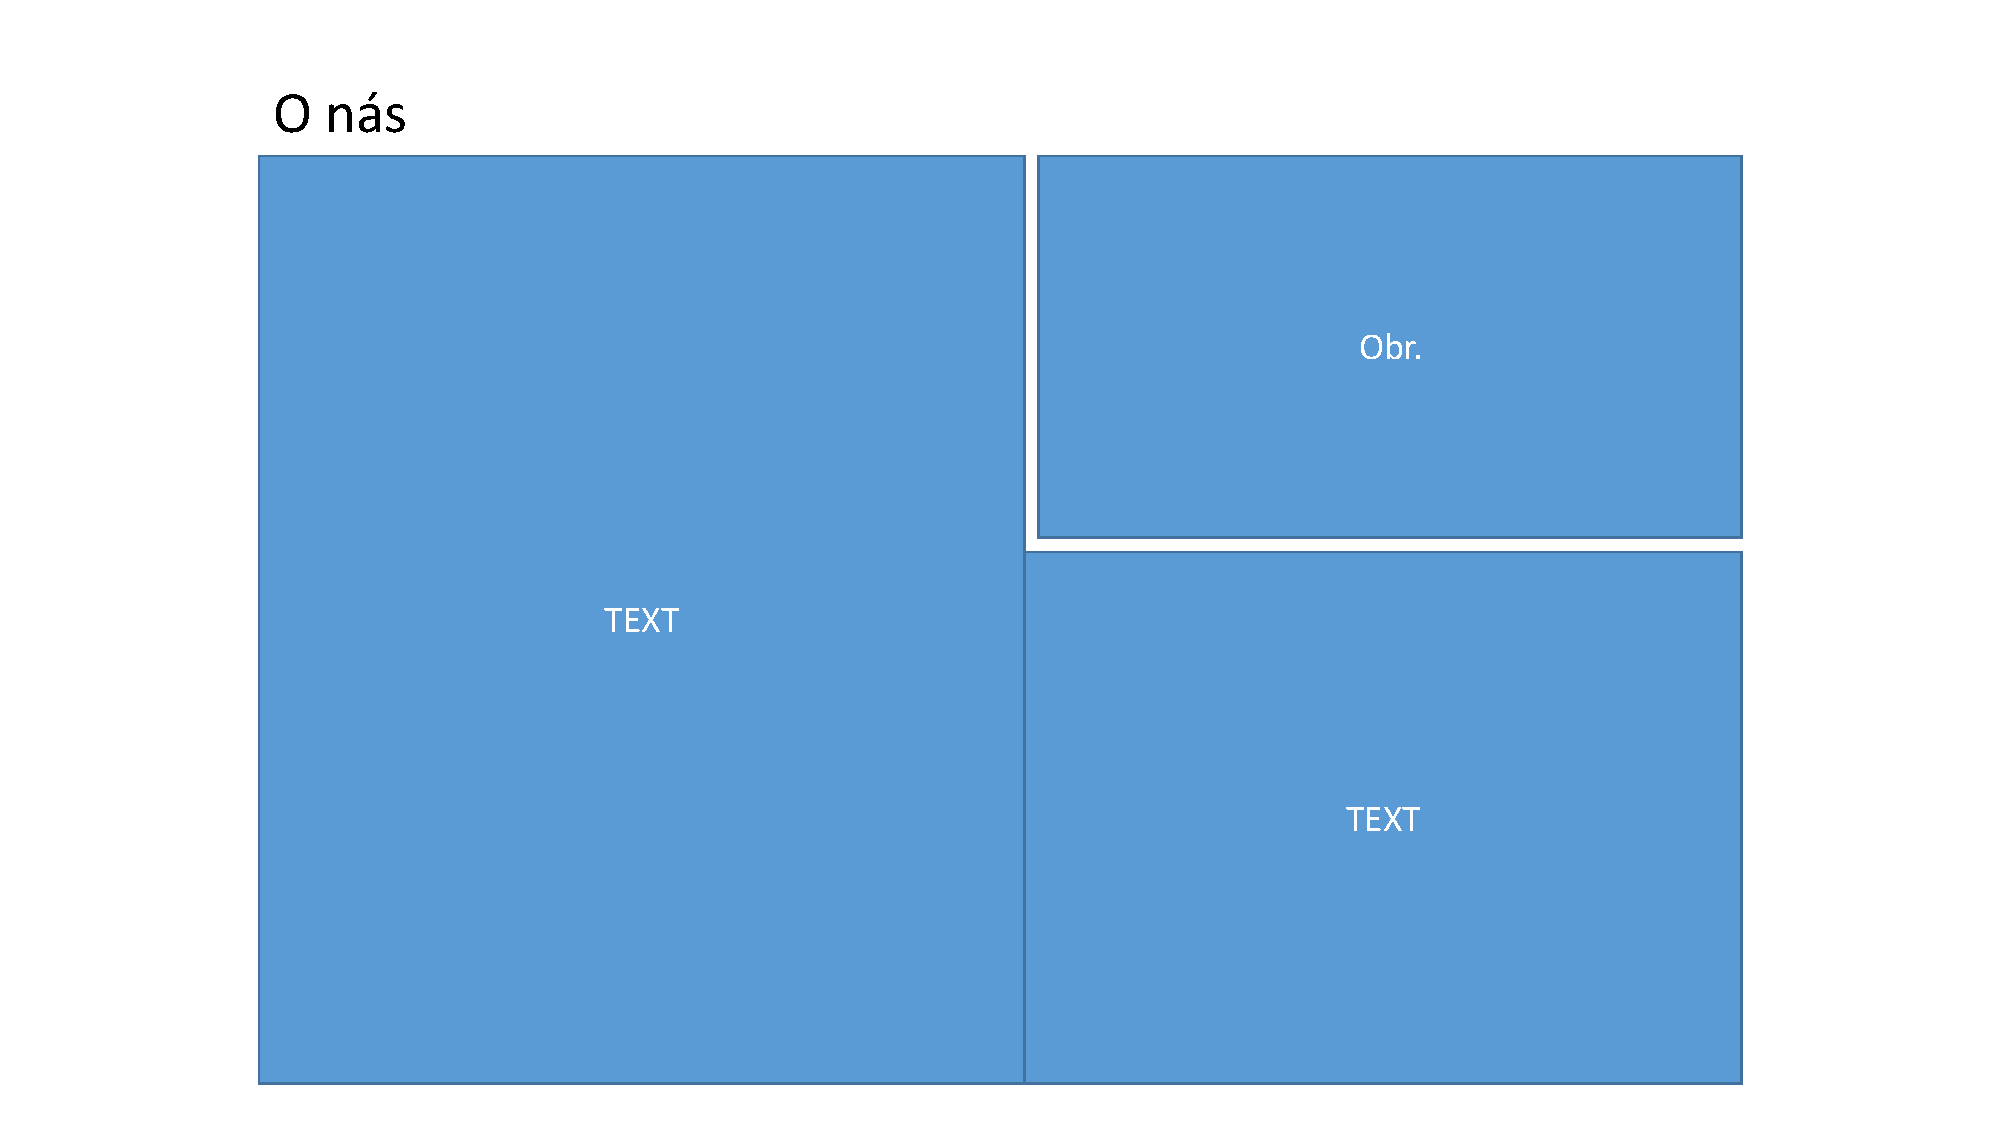
\includegraphics[width=140mm]{../img/UI concept/about}
\caption{Sekcia O~nás.}
\label{about}
\end{figure}

Sekcia~\uv{O~nás} by mala obsahovať text o~firme (napr.~jej histórii), príp.~nejaké fotky týkajúce sa firmy. Ďalej po~kliknutí na~odkaz~,,Kontakt`` v~navigácii alebo~po~kliknutí na~telefónne číslo v~hornej časti aplikácie (viď vpravo hore na~obr.~\ref{layout}) by mal byť užívateľ presmerovaný do~časti aplikácie s kontaktom na firmu, príp. pridružené firmy (viď~hranu~2 na~obr.\ref{p9 graph}). Pre~lepšiu predstavu sekcie~\uv{Kontakt} viď~obr.~\ref{contact}.

\begin{figure}[H]\centering

\includegraphics[width=140mm]{../img/UI concept/contact}
\caption{Sekcia Kontakt.}
\label{contact}
\end{figure}

Sekcia~\uv{Kontakt} by mala obsahovať tabuľku s~kontaktom (telefónne číslo a~emailová adresa) firmy. Okrem kontaktu klientskej firmy by mohla tabuľka obsahovať aj kontakty na iné (pridružene) firmy.

\section{Splnenie P5, P7 a~správa predmetov}
\label{splnenie p5 p7 a sprava predmetov}

\textbf{Pohľad pre~administrátorov:} Po~kliknutí na~odkaz~,,Správa webu`` v~navigácii, ktorý by mal byť viditeľný iba pre~administrátorov, by mal byť administrátor presmerovaný do~sekcie Správa webu (viď~hranu~1 na~obr.~\ref{p5 p7 a sprava predmetov graph}). Tá by mala vyzerať následovne: v~hornej časti by sa mal nachádzať panel s~kartami, ktorými by sa mal byť administrátor schopný preklikávať (viď hrany 2 až 9 na obr. \ref{p5 p7 a sprava predmetov graph}), a~pod~panelom by sa mal nachádzať obsah podľa toho, na~akej karte sa administrátor nachádza.

\begin{figure}[H]\centering
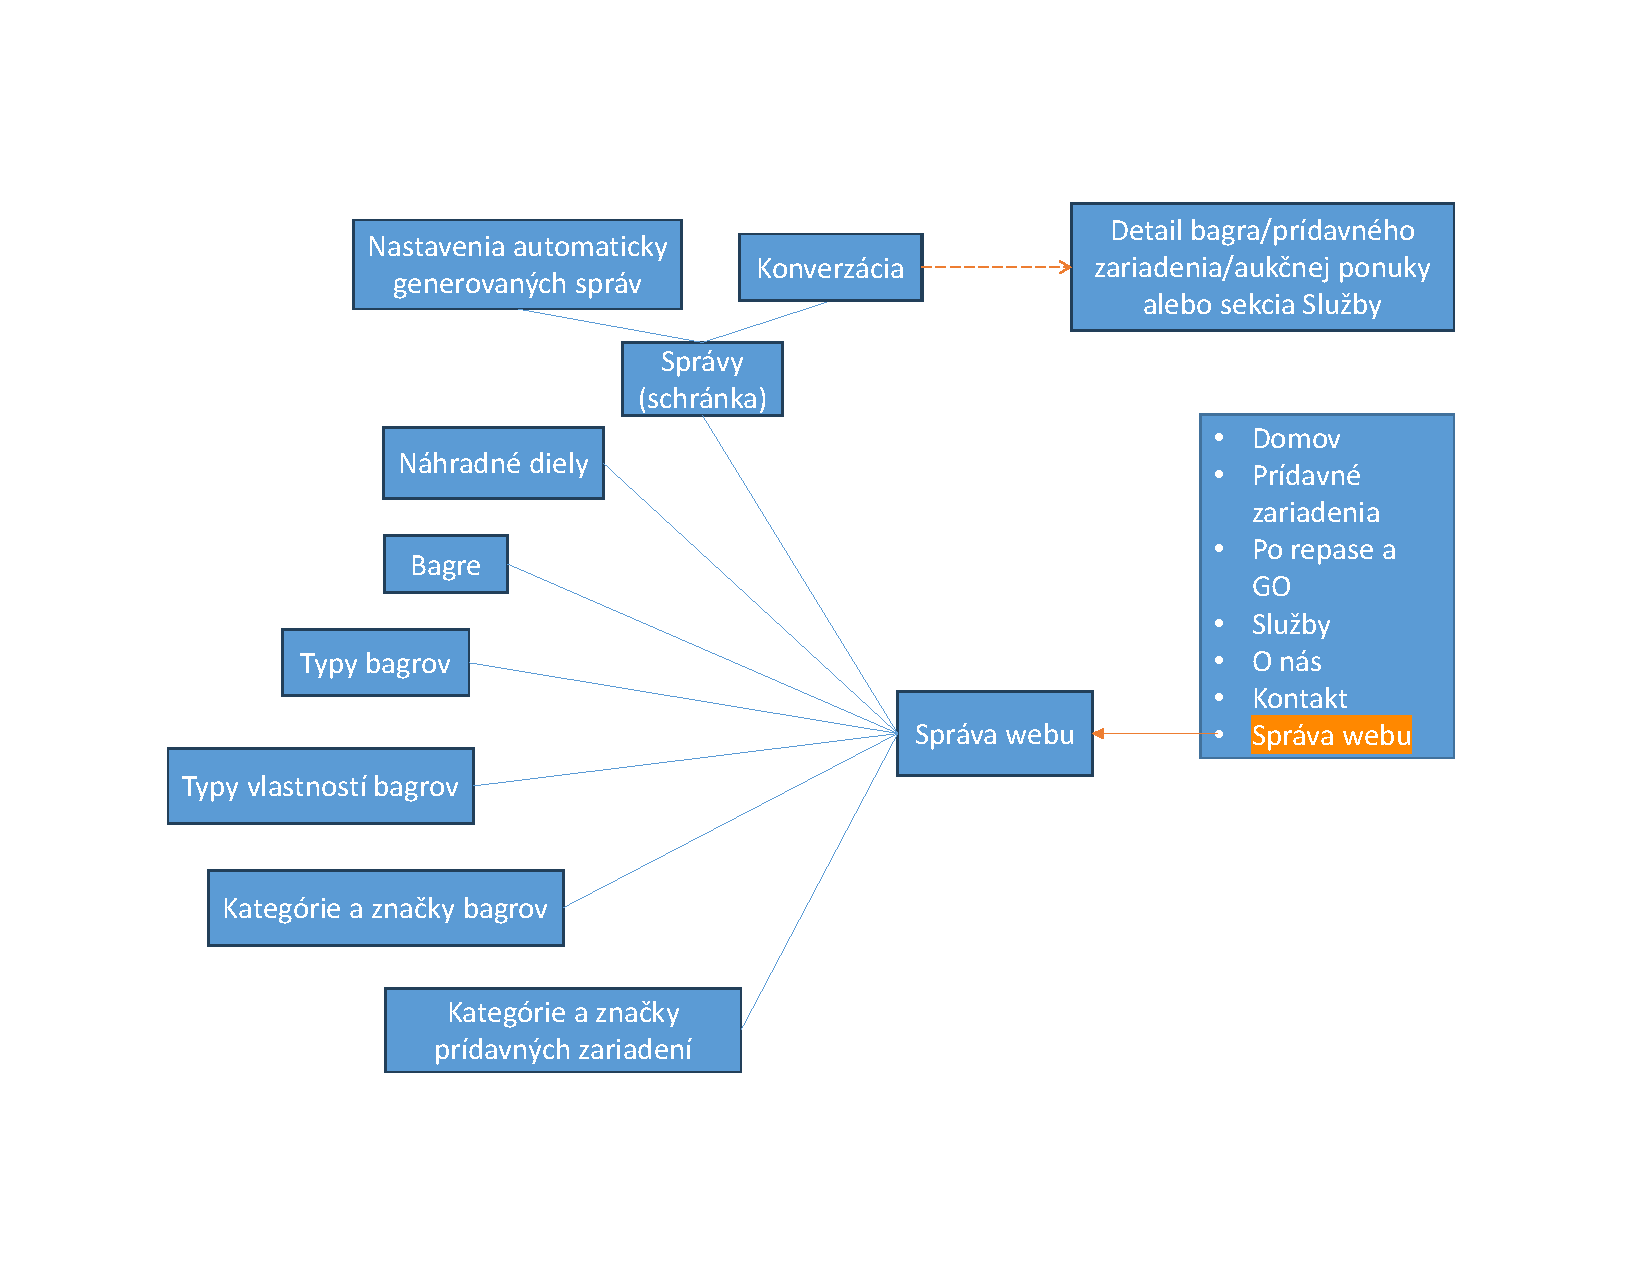
\includegraphics[width=140mm]{../img/UI concept/p5 p7 a sprava predmetov graph}
\caption{Prechádzanie medzi časťami aplikácie spĺňajúcimi požiadavku P5 (orientovaná hrana značí prechod do~novej časti aplikácie, neorientovaná prepínanie medzi časťami, prerušovaná nepovinný prechod do~novej časti).}
\label{p5 p7 a sprava predmetov graph}
\end{figure}

Po príchode do~tejto časti by sa mala administrátorovi zobraziť prvá karta~-- ,,Správy`` (viď~hranu~2 na~obr.~\ref{p5 p7 a sprava predmetov graph}). Okrem tejto karty by sa mal byť administrátor schopný prekliknúť na karty: ,,Náhradné diely`` (hrana~3 na~obr.~\ref{p5 p7 a sprava predmetov graph}), ,,Bagre`` (hrana~4 na~obr.~\ref{p5 p7 a sprava predmetov graph}), ,,Typy bagrov`` (hrana~5 na~obr.~\ref{p5 p7 a sprava predmetov graph}), ,,Typy vlastností bagrov`` (hrana~6 na~obr.~\ref{p5 p7 a sprava predmetov graph}), ,,Kategórie a~značky bagrov`` (hrana~7 na~obr.~\ref{p5 p7 a sprava predmetov graph}), ,,Kategórie a~značky prídavných zariadení`` (hrana~8 na~obr.~\ref{p5 p7 a sprava predmetov graph}).

Na~karte~,,Správy`` by mali byť vylistované konverzácie. Po~kliknutí na~nejakú z~konverzácií by sa mala administrátorovi zobraziť konverzácia (viď~hranu~9 na~obr.~\ref{p5 p7 a sprava predmetov graph}). Ak by bola konverzácia odoslaná z~našeho systému, malo by byť v~tejto konverzácii vložené prepojenie do~časti aplikácie z~ktorej bola správa odoslaná (viď~hranu~10 na~obr.~\ref{p5 p7 a sprava predmetov graph}). Mohla by to byť časť aplikácie s~detailom bagra, detailom prídavného zariadenia, detailom aukčnej ponuky alebo~sekcia Služby. Okrem toho by sa mal byť administrátor schopný dostať z~karty~,,Správy`` (pomocou tlačidla~,,Nastavenia``, ktoré by sa malo na~karte nachádzať) do~časti aplikácie s~nastaveniami automaticky generovaných správ (viď~hranu~11 na~obr.~\ref{p5 p7 a sprava predmetov graph}).

\subsection{Karta Správy~-- schránka}
\label{karta spravy schranka}

\textbf{Pohľad pre~administrátorov:} Po~príchode do~sekcie~,,Správa webu`` alebo~po~kliknutí na~kartu~,,Správy`` v~sekcii~,,Správa webu`` by sa mala administrátorovi zobraziť emailová schránka podobná Gmailu. Pre~lepšiu predstavu tejto časti aplikácie viď~obr.~\ref{messages}.

\begin{figure}[H]\centering
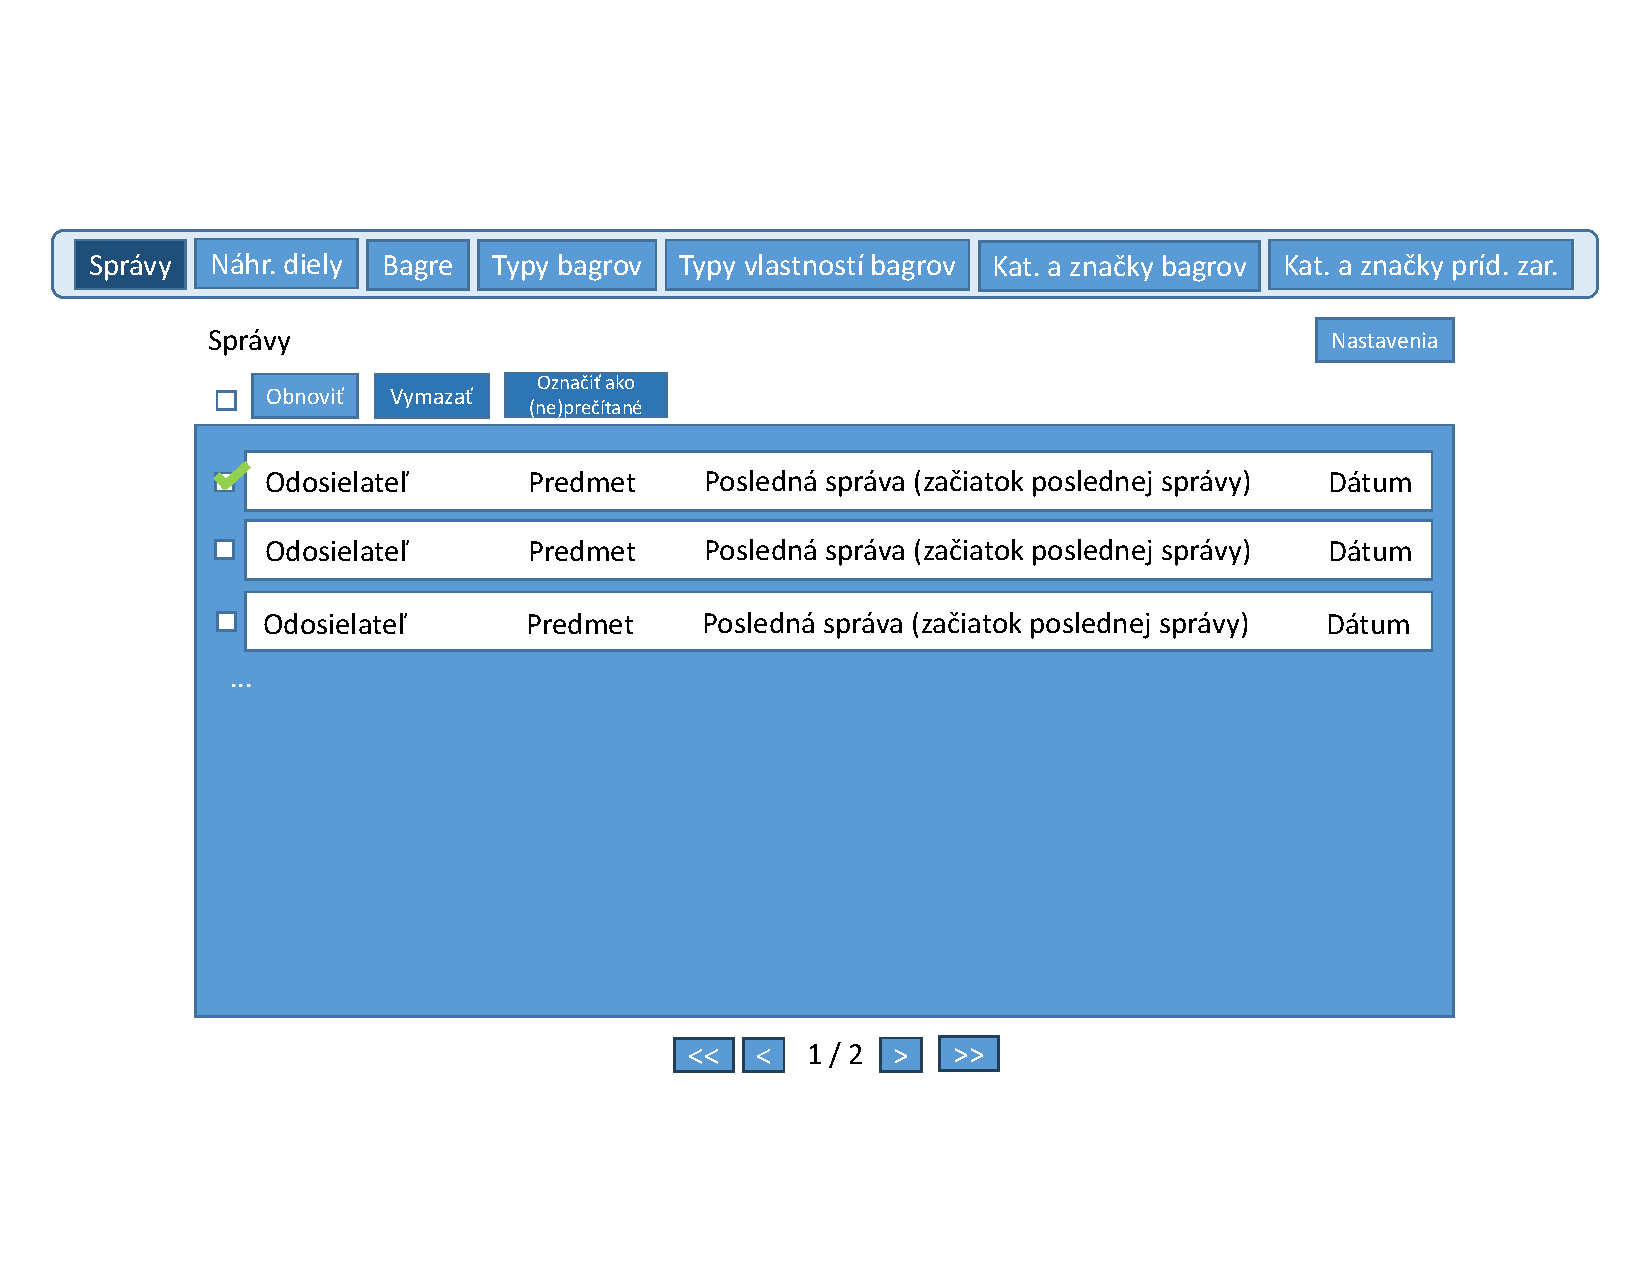
\includegraphics[width=140mm]{../img/UI concept/messages}
\caption{Emailová schránka.}
\label{messages}
\end{figure}

V~schránke by mali byť vylistované konverzácie (vlákna správ) zhora dole od~najnovšej po~najstrašiu. Každá takáto konverzácia by mala byť reprezentovaná riadkom, v~ktorom by malo byť uvedené meno odosielateľa, predmet a~text poslednej správy (resp.~jeho začiatok v~prípade dlhšieho textu), a~dátum poslednej správy (emailu v~konverzácii). Vedľa každého riadka konverzácie by malo byť začiarkovacie políčko, ktorým vieme konverzáciu označiť. Po~kliknutí na~nejaký z~riadkov by sa mala administrátorovi zobraziť vybraná konverzácia.

Vylistované konverzácie by mali byť stránkované (max.~osem konverzácii na~stránku). Pod~vylistovanými konverzáciami by malo byť tlačidlo~\uv{<<}, ktoré by malo byť schopné presunúť administrátora na~prvú stranu vylistovaných konverzácií, tlačidlo~\uv{<}, ktoré by malo byť schopné presunúť administrátora o~jednu stranu dopredu a~tlačidlá~\uv{>}, \uv{>>}, ktoré by mali fungovať analogicky (lenže na~opačnú stranu). Ak by sa administrátor nachádzal na~prvej strane, tak tlačidlá \uv{<<} a \uv{<} by nemali byť aktívne (nemalo by sa na ne dať kliknúť). Podobne ak by sa administrátor nachádzal na~poslednej strane, tlačidlá \uv{>} a \uv{>>} by nemali byť aktívne.

Nad~vylistovanými konverzáciami by mal byť nadpis~,,Správy`` a~tlačidlo~,,Nastavenia``, ktorým by sa mal byť administrátor schopný dostať do~časti aplikácie s~nastaveniami automaticky generovaých správ. Ďalej pod~nadpisom by malo byť začiarkovacie políčko, ktorým by mal byť administrátor schopný začiarknúť (označiť) všetky konverzácie na~aktuálnej strane. Okrem tohto začiarkovacieho políčka, by tam malo byť tlačidlo~,,Obnoviť`` a~ak by bola označená aspoň jedna konverzácia, tak potom by mali byť viditeľné aj tlačidlá~,,Vymazať`` a~,,Označiť ako prečítané`` alebo~,,Označiť ako neprečítané``.

Tlačidlo~,,Označiť ako neprečítané`` by sa malo zobraziť vtedy, keď sú všetky označené správy prečítané. Tlačidlo~,,Označiť ako prečítané`` by sa malo zobraziť vtedy, keď sú všetky označené správy neprečítané alebo~sú medzi správami aj prečítané, aj neprečítané správy.

Tlačidlom~,,Vymazať`` by mal byť administrátor schopný vymazať označené konverzácie. Po~kliknutí naň sa má zobraziť potvrdzovacie modálne okno s~nadpisom~,,Vymazať vybrané konverzácie`` a~textom~\uv{Naozaj chcete vymazať vybrané konverzácie natrvalo?}.

\subsection{Karta Správy~-- konverzácia}

\textbf{Pohľad pre~administrátorov:} Po~kliknutí na~nejakú z~konverzácií by sa mala administrátorovi zobraziť daná konverzácia. Pre~lepšiu predstavu tejto časti aplikácie viď~obr.~\ref{message}.

\begin{figure}[H]\centering
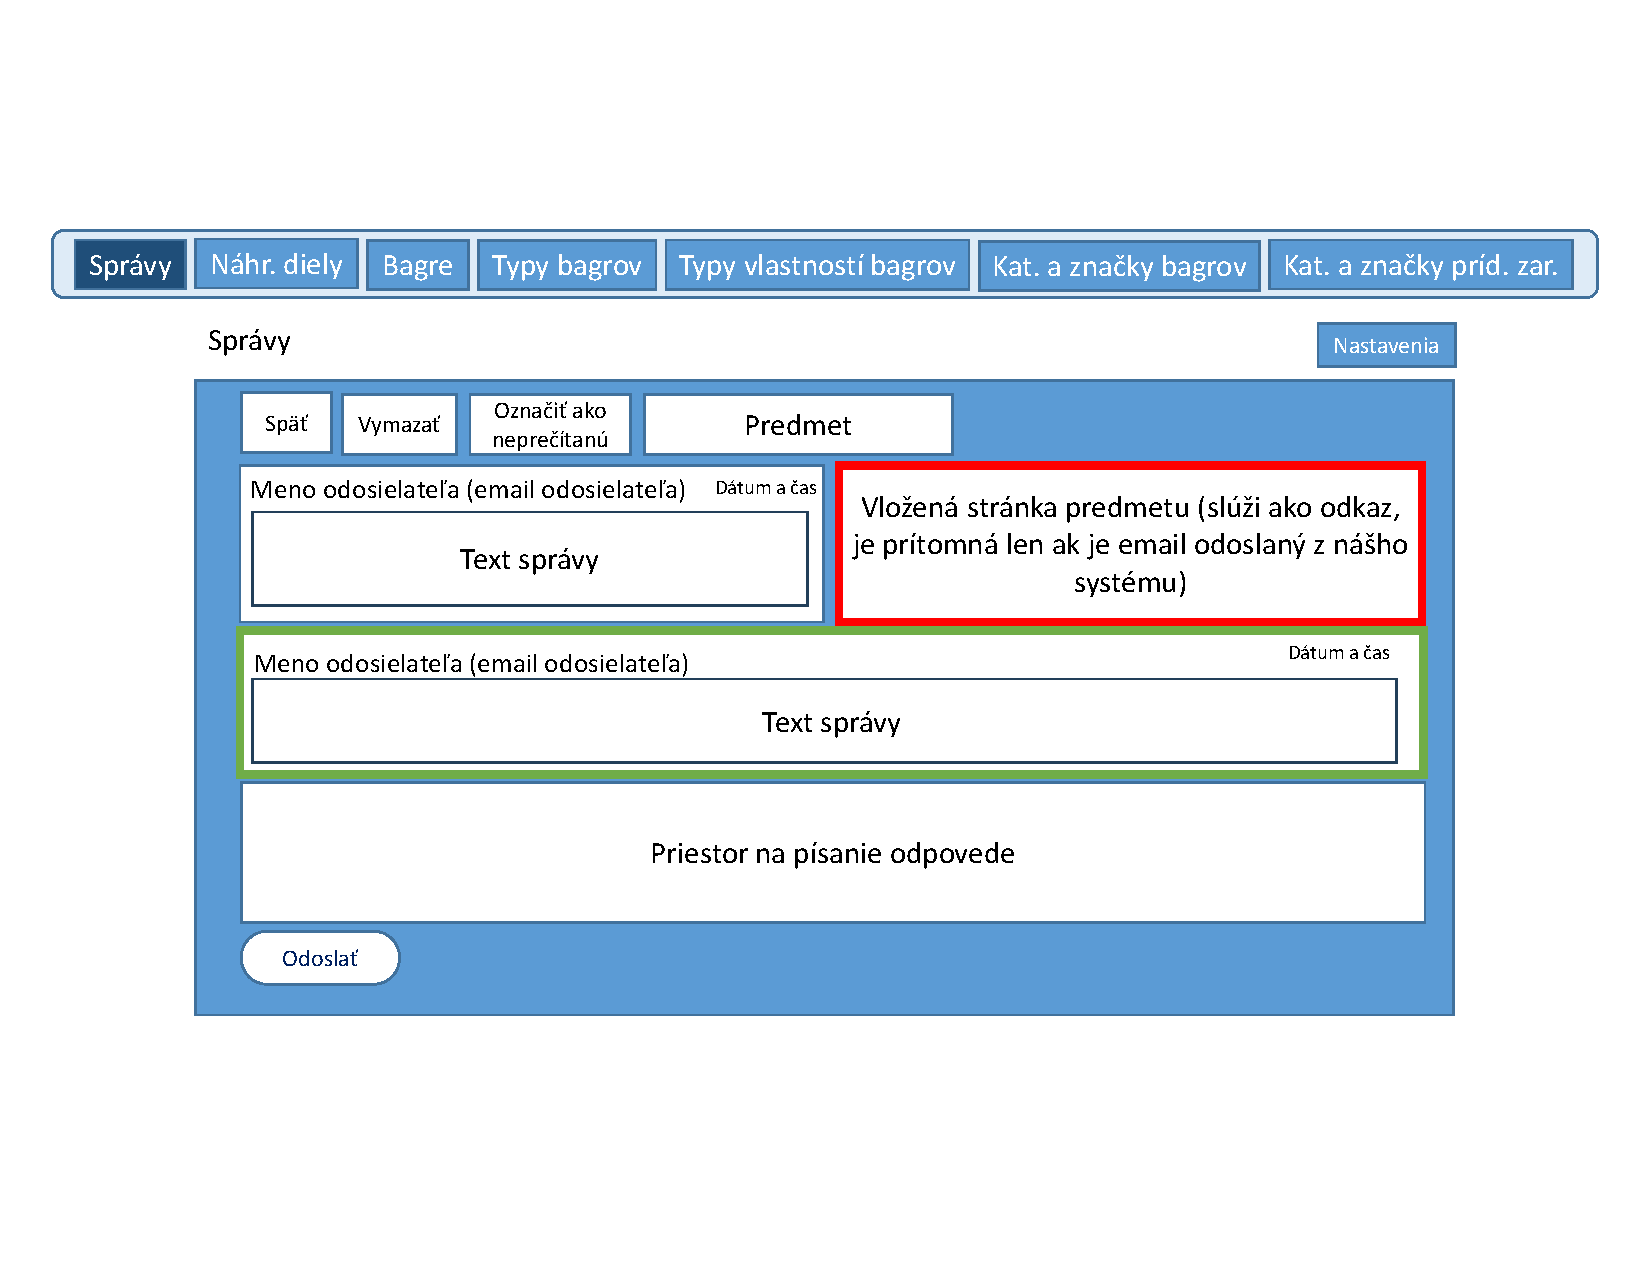
\includegraphics[width=140mm]{../img/UI concept/message}
\caption{Konverzácia.}
\label{message}
\end{figure}

V~hornej časti by sa mal nacházať nadpis~,,Správy`` a~tlačidlo~,,Nastavenia`` (pre~otvorenie nastavenia automaticky generovaných správ). Pod nimi by sa mali nachádzať tlačidlá~,,Späť`` (pre~návrat do~schránky), ,,Vymazať`` a~tlačidlo~,,Označiť ako neprečítanú`` (pre~označenie správy za~neprečítanú). Tlačidlom~,,Vymazať`` by mal byť administrátor schopný vymazať otvorenú konverzáciu. Po~kliknutí by sa malo zobraziť potvrdzovacie modálne okno s~nadpisom~,,Vymazať konverzáciu`` a~textom~\uv{Naozaj chcete vymazať túto konverzáciu natrvalo?}.

Napravo od~tlačidiel by mal byť zobrazený predmet (poslednej správy v~konverzácii). Pod~tlačidlami a~predmetom by mali byť zobrazené jednotlivé správy~(emaily) konverzácie zoradené zhora dole od~najstaršej po~najnovšiu. Ak by bola (prvá) správa odoslaná z~nášho systému, tak vedľa nej by mala byť vložená časť aplikácie, odkiaľ bola správa odoslaná (na~obr.~\ref{message} viď~časť označenú červeným rámom). Po~kliknutí na~túto časť by mal byť administrátor presmerovaný do~časti aplikácie, odkiaľ bola správa odoslaná (mala by sa otvoriť v~novom okne). V~prípade, že by správa nebola odoslaná z~nášho systému, mala by sa správa roztiahnuť na~šírku tejto časti aplikácie (rovnako ako je druhá správa, označená zeleným rámom, na~obr.~\ref{message}). Pre~každú správu v~konverzácii by sa malo zobraziť meno a~email odosielateľa, dátum a~čas správy, a~takisto text správy. Pod~vylistovanými správami by mal byť priestor pre~písanie odpovede a~tlačidlo~,,Odoslať``, ktorým by mal byť administrátor schopný odosielať správy do~konverzácie.

\subsection{Karta Správy~-- nastavenia automaticky generovaných správ}

\textbf{Pohľad pre~administrátorov:} Po~kliknutí na~tlačidlo~,,Nastavenia`` by sa mali administrátorovi zobraziť nastavenia automaticky generovaných správ. Pre~lepšiu predstavu tejto časti aplikácie viď~obr.~\ref{messages settings}.

\begin{figure}[H]\centering
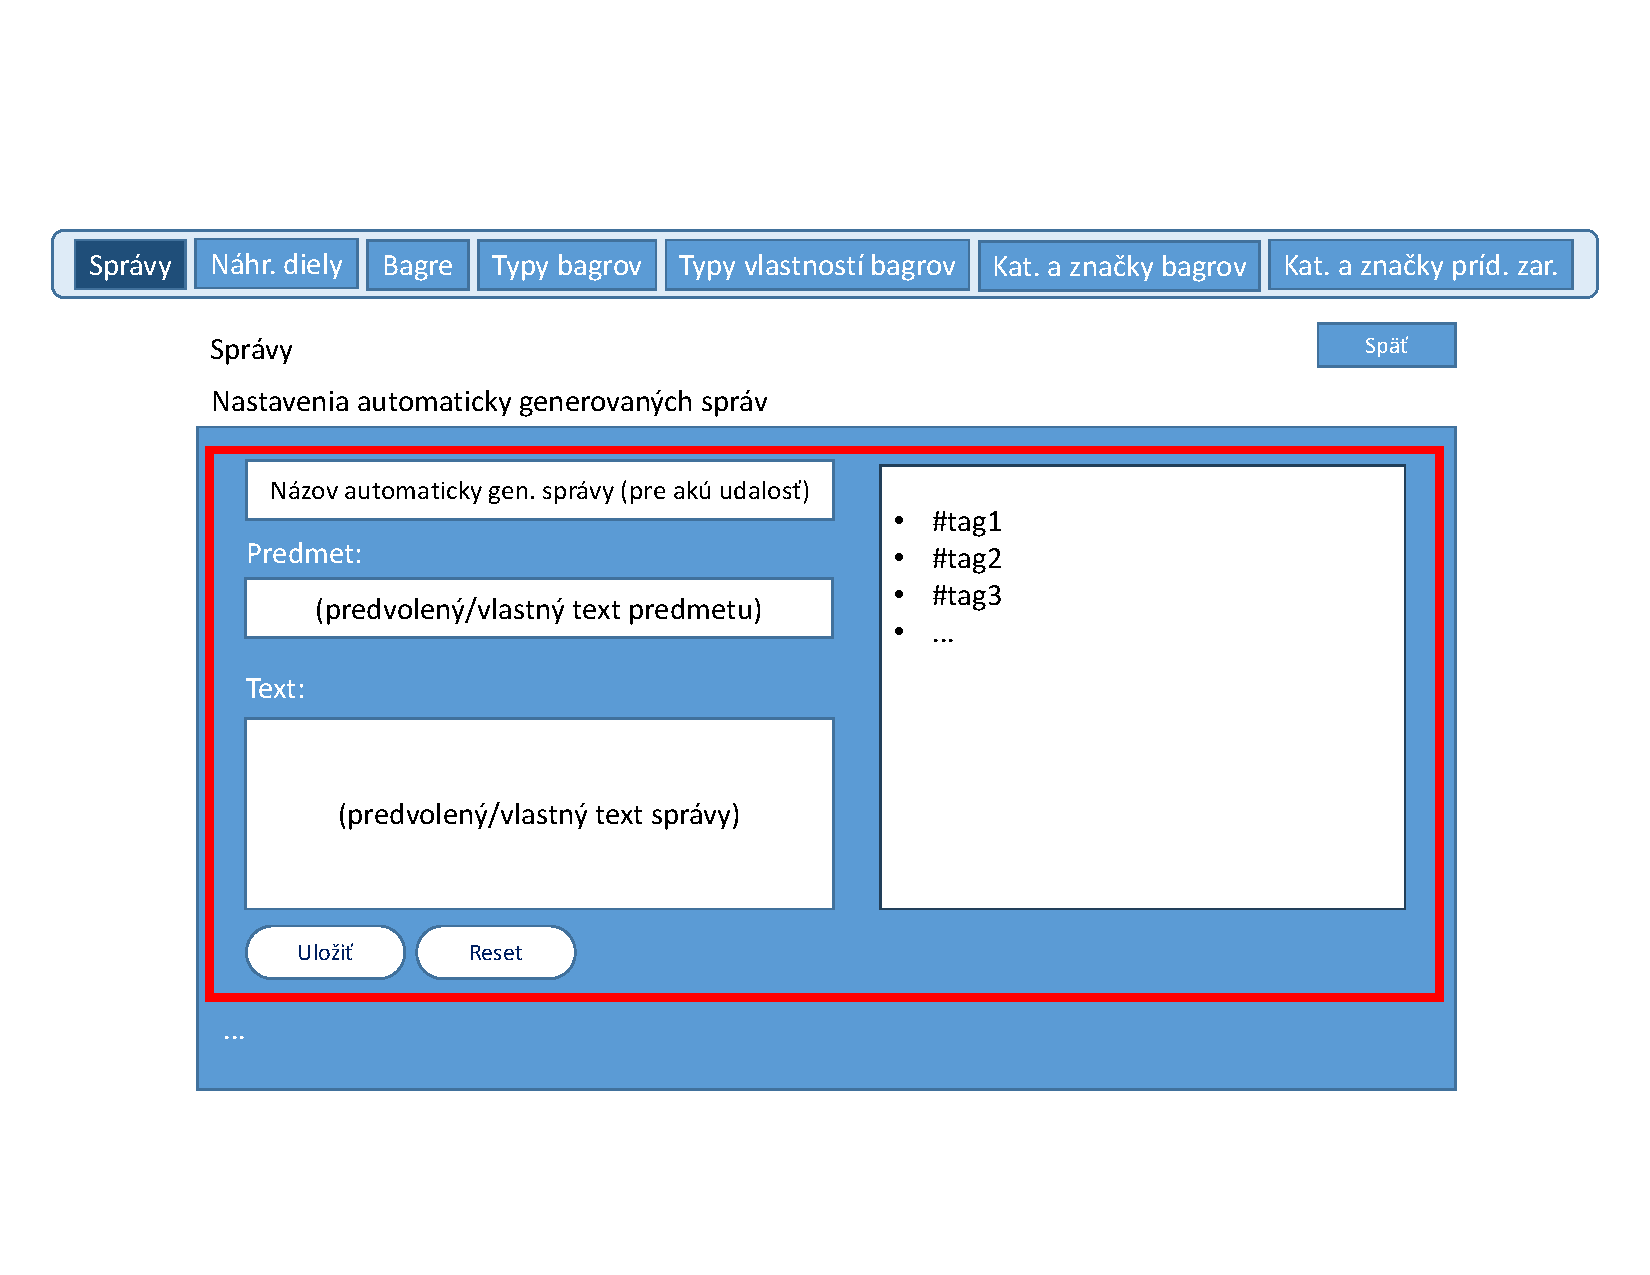
\includegraphics[width=140mm]{../img/UI concept/messages settings}
\caption{Nastavenia automaticky generovaných správ.}
\label{messages settings}
\end{figure}

Vo~vrchnej časti by sa mal nachádzať nadpis~,,Správy`` a~tlačidlo~,,Späť``, ktoré by malo byť schopné schovať (zatvoriť) nastavenia. Pod~nimi by sa mal nachádzať nadpis~,,Nastavenia automaticky generovaných správ`` a~sekcia, kde by sa pre~každú automaticky generovanú správu mala zobraziť časť, kde by sa dal nastavovať jej tvar (jedna zo~spomínaných častí je vyznačená červeným rámom na~obr.~\ref{messages settings}).

Každá z~takýchto častí by mala obsahovať názov automaticky generovanej správy (resp.~pre koho, akú udalosť je určená, napr.~,,Pre~víťaza aukcie``). Ďalej by mala obsahovať šablónu predmetu, šablónu textu a~v~pravej časti zoznam tagov povolených v~danej automaticky generovanej správe.

Tag by mal mať tvar ,,\#\{názov tagu\}``, kde názov tagu by mal obsahovať iba písmená a~znak ,,\_``. Pomocou tagov by mal byť administrátor schopný špecifikovať kde sa má v~texte (reps.~predmete) automaticky generovanej správy nachádzať konkrétna hodnota špecifikovaná tagom. Napr.~ak by sme použili vetu~,,Gratulujeme, vyhrali ste \#nazov\_stroja`` ako šablónu predmetu, tak email, ktorý by prišiel užívateľovi by mohol vyzerať takto:~,,Gratulujeme, vyhrali ste Stroj123`` (ak by bol názov výherného stroja ,,Stroj123``).

Každá z~automaticky generovaných správ by mala mať predvolený text, ktorý by mal byť administrátor schopný prepísať pomocou šablón. Ak by neboli definované vlastné šablóny, mali by sa využívať predvolené, a~preto by sa mali v~spomínaných poliach pre~predmet a~text zobrazovať predvolené šablóny. Ak by boli predvolené šablóny prepísané a~neskôr vymazané, tak polia by sa mali znova napĺniť predvolenými hodnotami. Ďalej pod~poliami by sa mali nachádzať tlačidlá~,,Uložiť`` (pre~uloženie šablón) a~,,Reset`` (pre~navrátenie k~predvoleným hodnotám).

\subsection{Karta Náhradné diely}
\label{karta nahradne diely}

\textbf{Pohľad pre~administrátorov:} Po prekliknutí na kartu \uv{Náhradné diely} v sekcii Správa webu by sa mala administrátorovi zobraziť časť aplikácie, kde by mal byť schopný spravovať (vytvárať, upravovať a mazať) náhradné diely. Pre lepšiu predstavu tejto časti viď obr. \ref{spare parts management}.

\begin{figure}[H]\centering
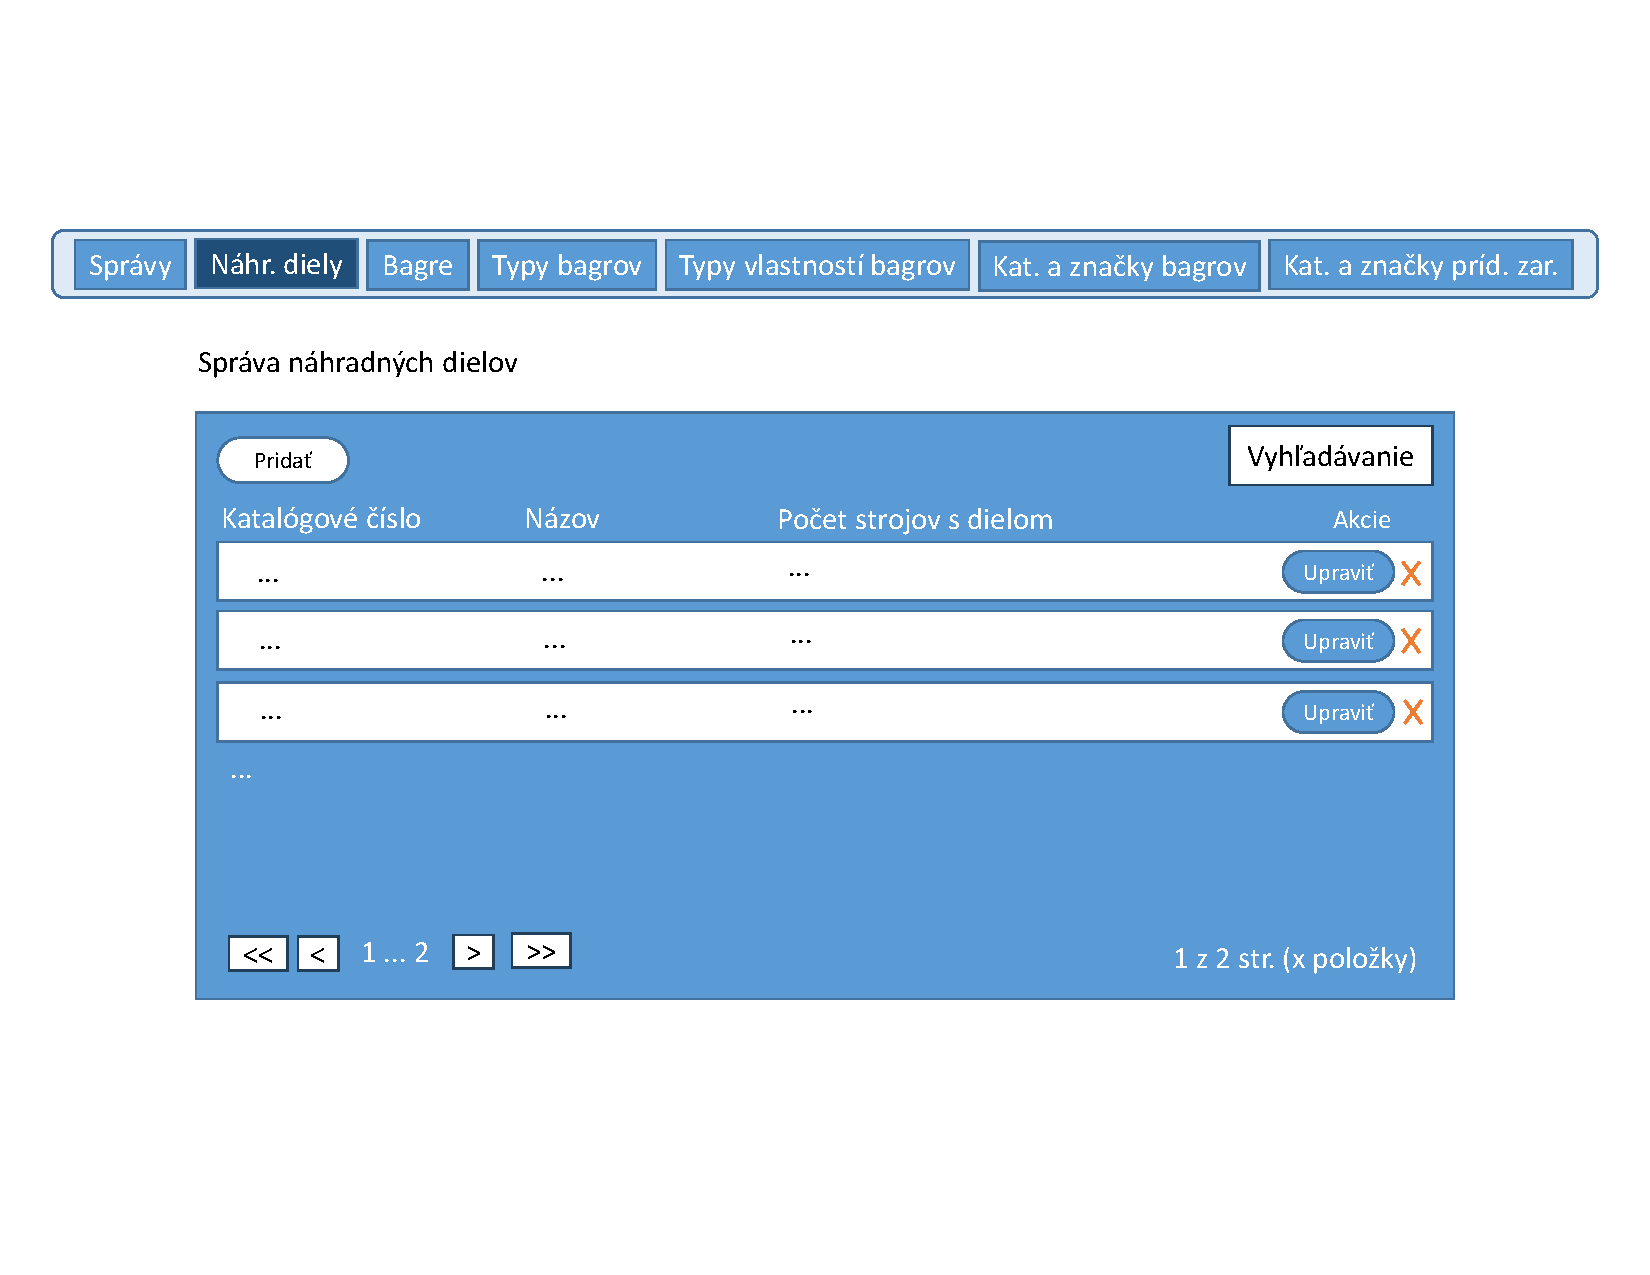
\includegraphics[width=140mm]{../img/UI concept/spare parts management}
\caption{Správa náhradných dielov.}
\label{spare parts management}
\end{figure}

Pod panelom s kartami by sa mal nachádzať nadpis \uv{Správa náhradných dielov}, a pod ním by sa mala nachádzať tabuľka s vylistovanými záznamami náhradných dielov. Tabuľka by mala obsahovať stĺpce pre katalógové číslo, názov a počet strojov s daným náhradným dielom. Každý záznam (riadok) náhradného dielu v tabuľke by mal zobrazovať tieto údaje. Vedľa týchto stĺpcov by mal existovať aj stĺpec pre akcie, v ktorom by pre každý záznam boli zobrazené dve tlačidlá~- \uv{Upraviť} a \uv{X}.

Tlačidlo \uv{X} slúží na vymazanie záznamu. Po jeho stlačení by sa malo zobraziť modálne potvrdzovacie okno s~nadpisom~,,Vymazať záznam`` a~textom \uv{Naozaj chcete tento záznam vymazať natrvalo?}. Ďalej po kliknutí na~tlačidlo \uv{Upraviť} alebo po dvojitom kliknutí na záznam (riadok v~tabuľke) by sa mal zobraziť formulár ako modálne okno s vyplnenými údajmi o vybranom náhradnom diele. Pomocou tohto formulára by mal byť administrátor schopný daný náhradný diel upravovať. Pre lepšiu predstavu formulára viď obr. \ref{spare part form}.

\begin{figure}[H]\centering
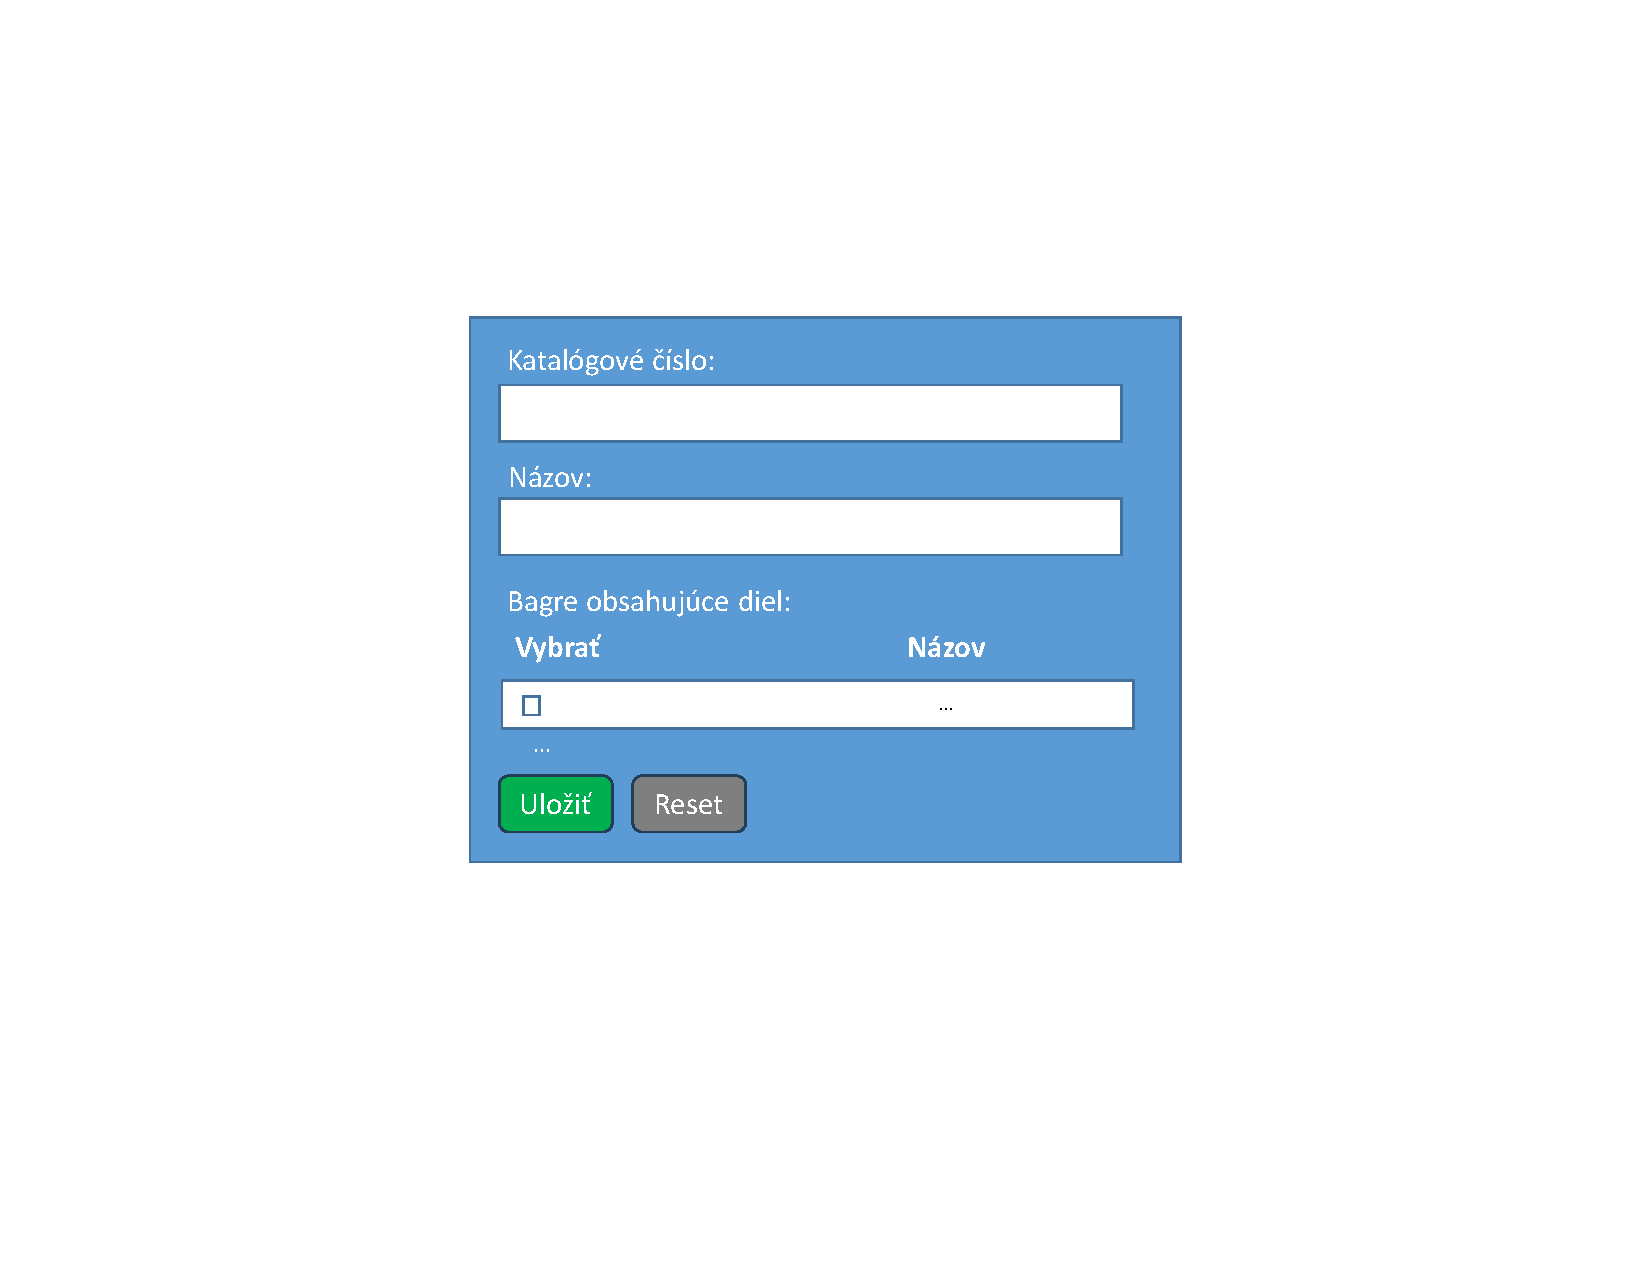
\includegraphics[width=140mm]{../img/UI concept/spare part form}
\caption{Formulár náhradného dielu.}
\label{spare part form}
\end{figure}

Formulár náhradného dielu by mal obsahovať polia pre katalógové číslo a~názov náhradného dielu, ktoré sú povinné. Taktiež by mal formulár obsahovať vylistované bagre. Vedľa názvu bagra by malo existovať začiarkovacie políčko. Ak stroj obsahuje daný náhradný diel, mal by administrátor políčko začiarknuť. Ďalej formulár obsahuje tlačidlá \uv{Uložiť} (pre uloženie zmien) a \uv{Reset} (pre vyprázdenie obsahu formulára). Ak by nejaké z polí po kliknutí na tlačidlo \uv{Uložiť} obsahovalo neplatné hodnoty, napr. by bolo nejaké z povinných polí prázdne, tak by sa pri danom poli mala zobraziť odpovedajúca chybová správa.

Podobne by sa mal po kliknutí na tlačidlo \uv{Pridať}, ktoré by sa malo nachádzať v~ľavej hornej časti tabuľky, zobraziť prázdny formulár náhradného dielu ako modálne okno, kde by mal byť administrátor schopný vytvoriť nový záznam náhradného dielu. V pravej hornej časti tabuľky by sa malo nachádzať pole pre vyhľadávanie záznamov v~tabuľke. Ak by administrátor napísal do tohto poľa nejakú hodnotu, tak by sa vyhľadávala vo všetkých stĺpcov tabuľky okrem stĺpca pre počet strojov s dielom. Ďalej kliknutím na názov stĺcpa by mal byť administrátor schopný zoradiť záznamy vzostupne podľa hodnôt v danom stĺpci. Opätovným kliknutím na názov stĺpca by sa mali záznamy zoradiť zostupne podľa hodnôt v danom stĺpci. Ak by administrátor klikol tretíkrát na~ten istý názov stĺpca, poradie záznamov by sa malo vrátiť do pôvodného stavu ako bolo pred prvým kliknutím. Ak by už boli záznamy zoradené podľa stĺpca X a administrátor by klikol na názov iného stĺpca Y, záznamy by sa mali zoradiť (iba) podľa stĺpca Y.

Navyše záznamy v tabuľke by mali byť stránkované. Maximálny povolený počet zobrazených záznamov na stránku by mal byť päť. V ľavej spodnej časti tabuľky by sa mal nachádzať panel s číslami strán, na ktoré by sa malo dať kliknúť a presunúť tak na danú stranu. Okrem čísel strán by sa tam mali nachádzať tlačidlá \uv{<<}, \uv{<}, \uv{>}, \uv{>>}. Kliknutím na~tlačidlo~\uv{<<} by mal byť administrátor presunutý na~prvú stranu, kliknutím na tlačidlo~\uv{<} by mal byť administrátor presunutý o~jednu stranu dopredu. Tlačidlá~\uv{>} a \uv{>>} by mali fungovať analogicky (lenže na~opačnú stranu). Ak by sa administrátor nachádzal na~prvej strane, tak tlačidlá \uv{<<} a \uv{<} by nemali byť aktívne (nemalo by sa na ne dať kliknúť). Podobne ak by sa administrátor nachádzal na~poslednej strane, tlačidlá \uv{>} a \uv{>>} by nemali byť aktívne. Okrem toho by mal byť v~pravej spodnej časti tabuľky vypísaný údaj, že na akej strane sa adminitrátor nachádza, koľko je strán a koľko je vypísaných záznamov na~aktuálnej strane.

\subsection{Karty Bagre, Typy bagrov, Typy vlastností bagrov}
\label{karty bagre typy bagrov typy vlastnosti bagrov}

\textbf{Pohľad pre~administrátorov:} Tak ako by sa mal byť administrátor schopný prekliknúť na kartu Náhradné diely, tak by sa mal byť schopný prekliknúť aj na karty Bagre, Typy bagrov alebo Typy vlastností bagrov. Všetky tieto karty by mali byť skoro totožné s kartou Náhradné diely, ktorá bola opísaná v časti \ref{karta nahradne diely}. Líšiť by sa mali len v~nadpise (ktorý by sa mal nachádzať nad tabuľkou), v~stĺpcoch tabuľky (pochopiteľne aj stĺpcami, ktoré nie sú určené pre vyhľadávanie), pričom tabuľka na každej karte by mala obsahovať stĺpec pre akcie rovnako ako bolo spomenuté v opise karty Náhradné diely (viď v časti \ref{karta nahradne diely}). Takisto by sa mali líšiť aj formulárom pre vytvorenie alebo~úpravu záznamu. Teraz si prejdeme jednotlivé karty a detailnejšie opíšeme zmeny oproti karte Náhradné diely.

\begin{itemize}
\item \textbf{Karta Bagre}

Na~tejto karte by mal byť zobrazený nadpis~\uv{Správa bagrov} a~tabuľka obsahujúca stĺpce pre názov, kategóriu a značku bagra, a takisto údaj, či je bager určený iba pre aukciu. Nemalo by sa dať vyhľadávať podľa stĺpca, ktorý udáva, či je bager určený iba pre aukciu. Formulár pre vytvorenie, úpravu bagra by mal byť totožný s formulárom spomenutým v časti \ref{vytvorenie noveho a uprava existujuceho bagra} (formulár môžeme vidieť na~obr.~\ref{excavator form}, pričom nadpis nad formulárom by nemal byť súčasťou formulára).

\item \textbf{Karta Typy bagrov}

Táto karta by mala obsahovať nadpis~\uv{Správa typov bagrov} a tabuľku, ktorá by mala obsahovať stĺpce pre značku a kategóriu bagra, a taktiež počet bagrov daného typu. Nemalo by sa dať vyhľadávať podľa stĺpca pre počet bagrov. Pre lepšiu predstavu formulára pre vytvorenie, úpravu typu bagra viď~obr.~\ref{excavator type form}.

\begin{figure}[H]\centering
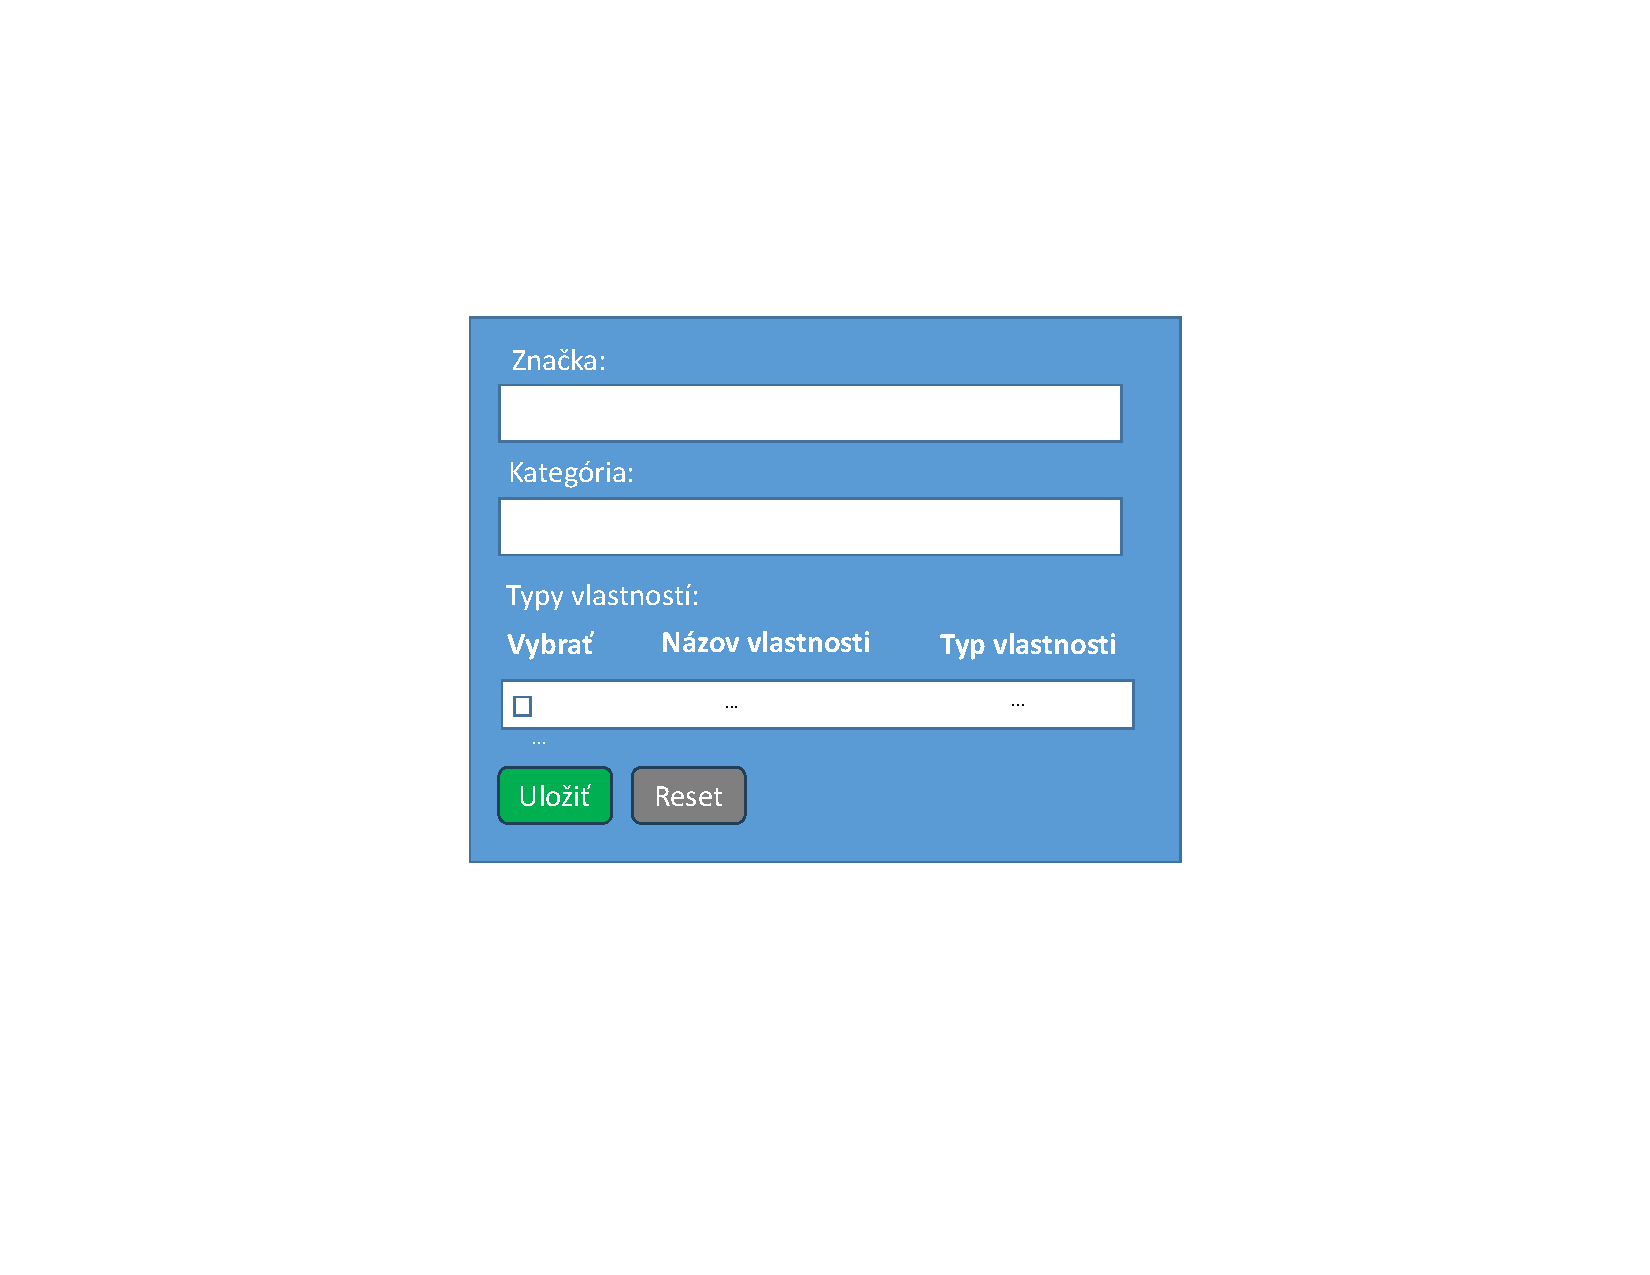
\includegraphics[width=140mm]{../img/UI concept/excavator type form}
\caption{Formulár typu bagra.}
\label{excavator type form}
\end{figure}

Formulár by mal obsahovať polia pre výber značky bagra a~kategórie bagra (obe údaje sú povinné), a taktiež vylistované typy vlastností bagra. Pre každý vylistovaný typ vlastnosti bagra je zobrazený jeho názov (napr. hmotnosť) a~typ (napr. číslo), pričom vedľa týchto údajov by malo byť začiarkovacie políčko. Pomocou týchto začiarkovacích políčok by mal byť administrátor schopný vybrať aké typy vlastností by mal mať vytváraný (resp. upravovaný) typ bagra. Ďalej by mal mať formulár v spodnej časti tlačidlá \uv{Uložiť} (pre uloženie záznamu) a~\uv{Reset} (pre vyprázdenie formulára). Ak by po~kliknutí na~tlačidlo \uv{Uložiť} nebolo nejaké z polí validné, napr.~by chýbala hodnota v nejakom z povinných polí, tak by sa pri danom poli mala zobraziť odpovedajúca chybová správa.

\item \textbf{Karta Typy vlastností bagrov}

Na tejto karte by mal byť nadpis~\uv{Správa typov vlastností bagrov} a~tabuľka obsahujúca stĺpce pre názov a typ vlastnosti, ale takisto aj stĺpec pre~údaj o počte typov bagrov s danou vlastnosťou. Nemalo by sa dať vyhľadávať podľa počtu typov bagrov s danou vlastnosťou. Pre lepšiu predstavu formulára pre vytvorenie, úpravu typu vlastnosti bagra viď~obr.~\ref{excavator property type form}.

\begin{figure}[H]\centering
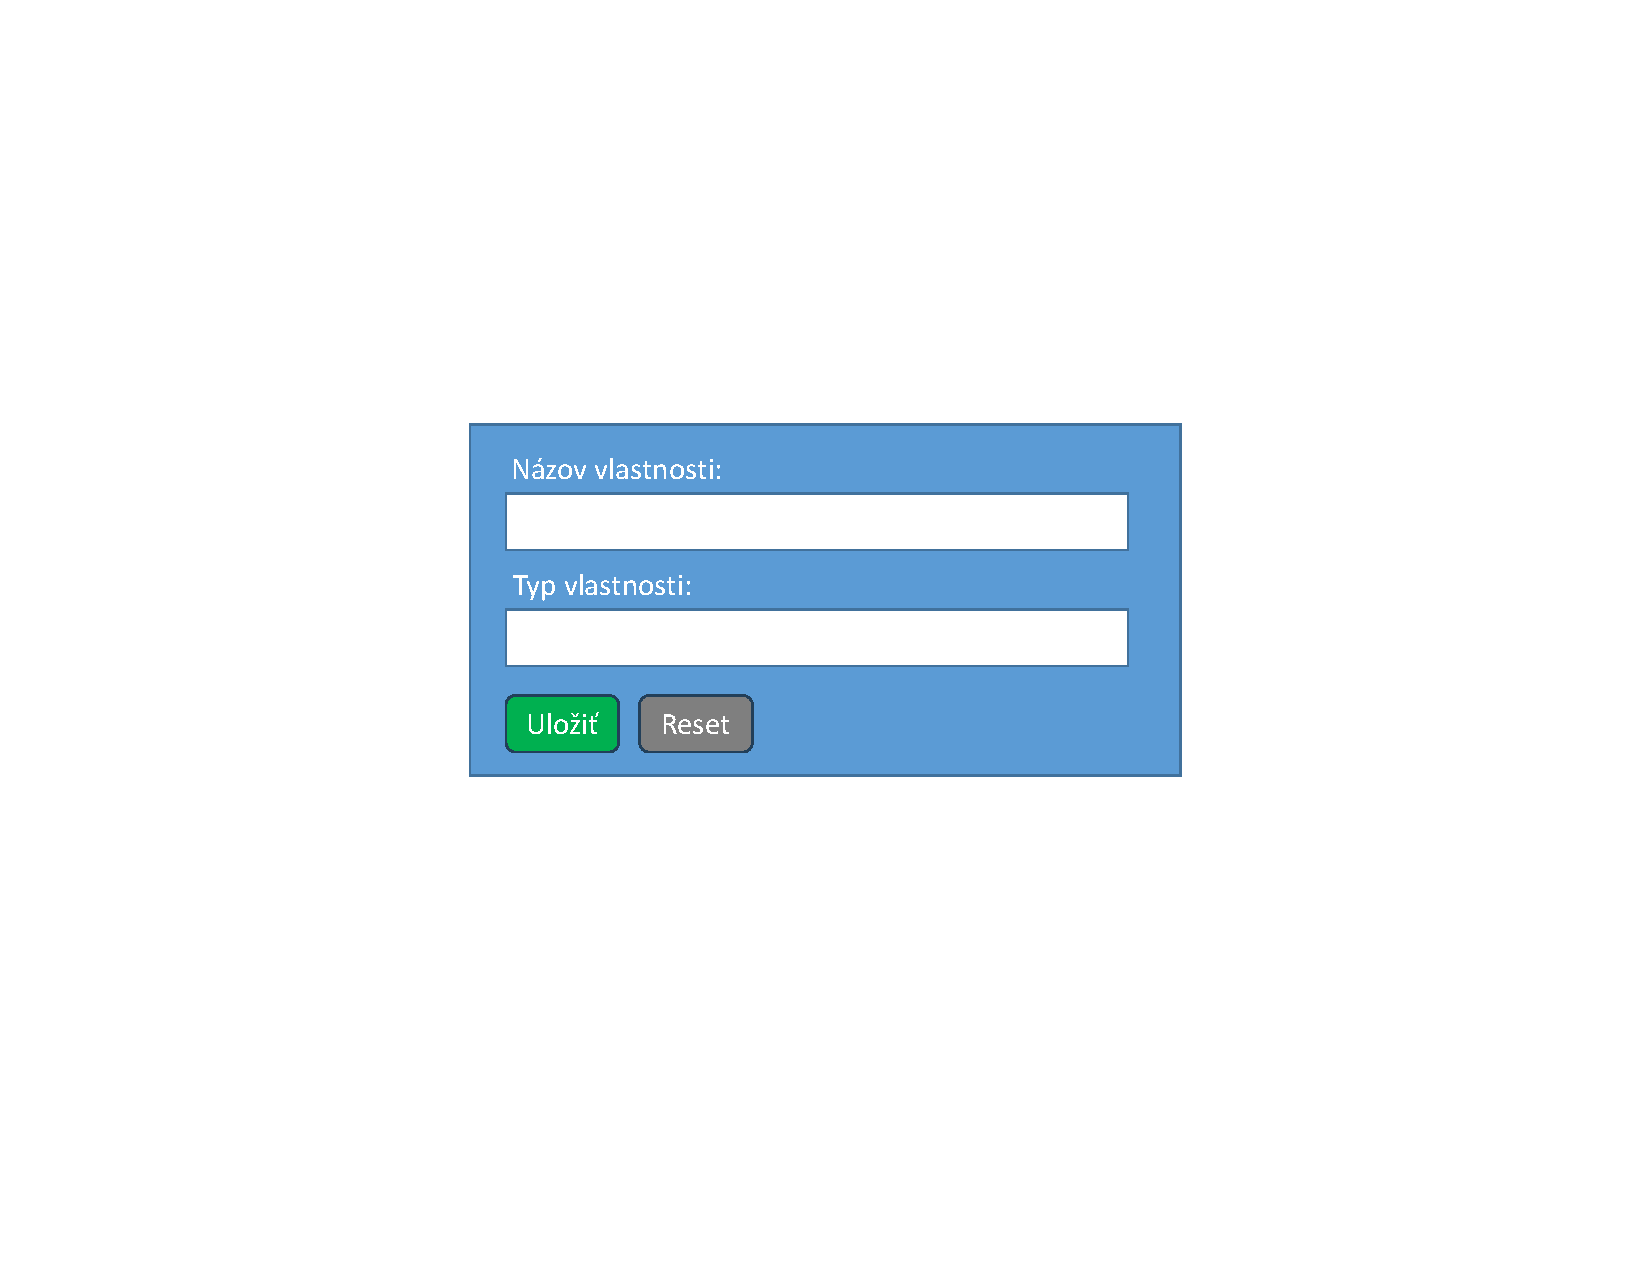
\includegraphics[width=140mm]{../img/UI concept/excavator property type form}
\caption{Formulár typu vlastnosti bagra.}
\label{excavator property type form}
\end{figure}

Formulár by mal obsahovať polia pre názov a výber typu vlastnosti bagra, pričom~obe údaje sú povinné. V spodnej časti formulára by mali byť tlačidlá~\uv{Uložiť} (pre~uloženie záznamu) a~\uv{Reset} (pre~vyprázdenie formulára). Ak by po~kliknutí na~tlačidlo \uv{Uložiť} chýbala v~nejakom z~polí hodnota, tak by sa pri danom poli mala zobraziť odpovedajúca chybová správa, ktorá by na to administrátora upozornila.

\end{itemize}

\subsection{Karty~Kategórie a~značky bagrov, Kategórie a~značky prídavných zariadení}

\textbf{Pohľad pre~administrátorov:} Rovnako ako by sa mal byť administrátor schopný prekliknúť na kartu Náhradné diely, tak by sa mal byť schopný prekliknúť aj na~kartu~Kategórie a~značky bagrov alebo~kartu~Kategórie a~značky prídavných zariadení. Tieto karty sa oproti karte Náhradné diely líšia, rovnako ako karty spomenuté v časti \ref{karty bagre typy bagrov typy vlastnosti bagrov}, v nadpise (ktorý sa nachádza nad tabuľkou), v~stĺpcoch tabuľky (pochopiteľne aj stĺpcami, ktoré nie sú určené pre vyhľadávanie), pričom stále platí, že tabuľka na každej karte by mala obsahovať stĺpec pre~akcie rovnako ako bolo spomenuté v opise karty Náhradné diely (viď~v~časti~\ref{karta nahradne diely}). Taktiež by sa mali líšiť aj~formulárom pre vytvorenie alebo~úpravu záznamu. No navyše platí, že tieto karty by mali obsahovať každá nie len jednu, ale~dve tabuľky. Jednu pre~kategórie bagrov a~druhú pre~značky bagrov (analogicky pre~kartu s~kategóriami a~značkami prídavných zariadení). Pre~lepšiu predstavu viď~obr.~\ref{excavator categories and brands management}. 

\begin{figure}[H]\centering
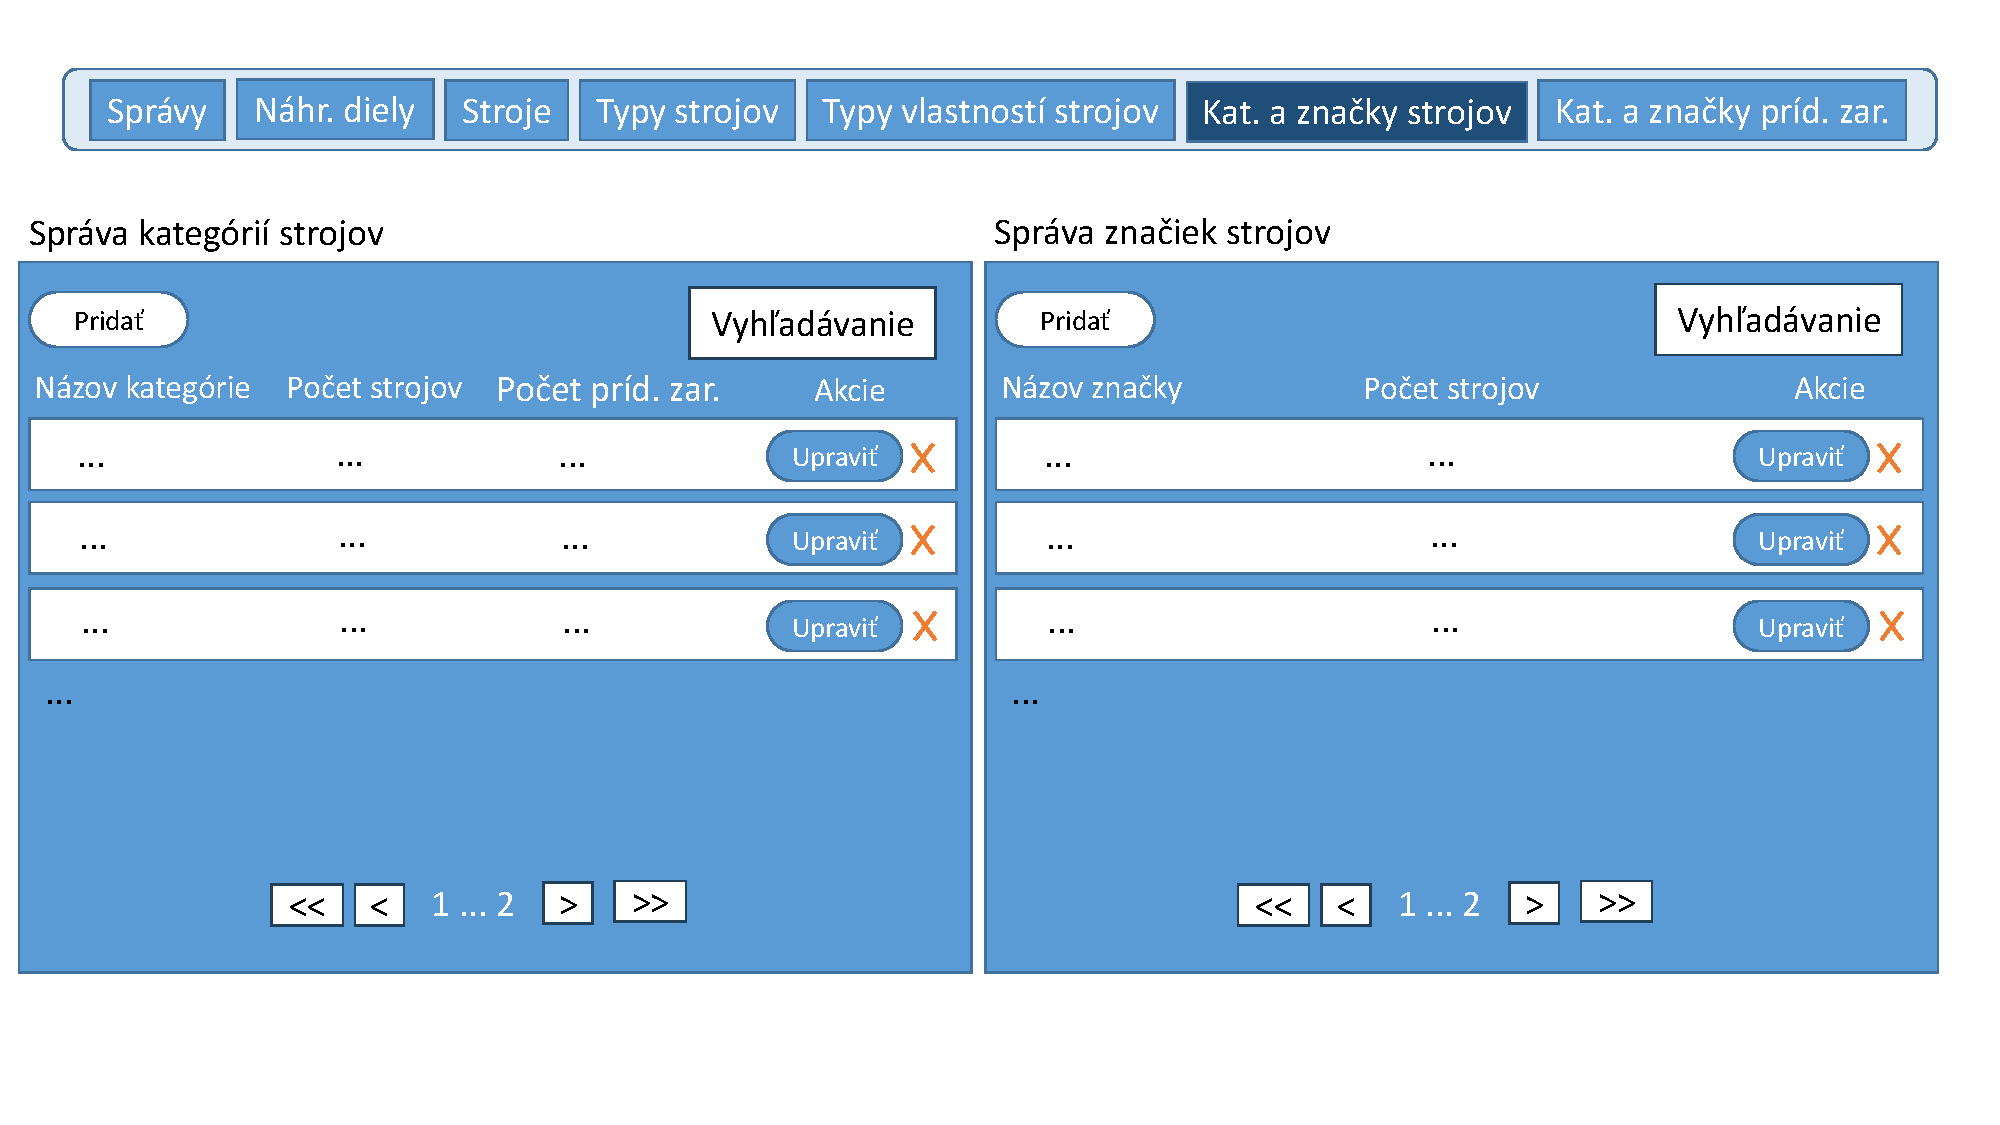
\includegraphics[width=140mm]{../img/UI concept/excavator categories and brands management}
\caption{Správa kategórií a značiek bagrov.}
\label{excavator categories and brands management}
\end{figure}

Táto zmena by mala existovať kvôli tomu, aby sa zmenšil počet kariet (malo by to viesť ku krajšiemu, prehľadnejšiemu užívateľskému rozhraniu), ale~takisto aj kvôli tomu, aby sa zamedzilo chybám spôsobenými zamenením tabuliek a~formulárov. Kategórie a značky bagrov aj~prídavných zariadení sú si koncepčne podobné a~ako uvidíme ďalej v texte, ich tabuľky a formuláre sú si tiež veľmi podobné. Preto by mala byť tabuľka so značkami bagrov a~tabuľka s~kategóriami bagrov na jednej karte a tabuľka so značkami prídavných zariadení a tabuľka s kategóriami prídavných zariadení na inej karte. Teraz si prejdeme a detailnejšie opíšeme zmeny oproti karte Náhradné diely jednotlivé karty podobne ako sme to spravili v časti \ref{karty bagre typy bagrov typy vlastnosti bagrov}.

\begin{itemize}
\item \textbf{Karta Kategórie a~značky bagrov}

Ako bolo spomenuté, na tejto karte sa nachádzajú dve tabuľky~-- jedna je pre~správu kategórií bagrov a druhá pre správu značiek bagrov. Obe si teraz opíšeme (opisovanú kartu je možné vidieť na obr. \ref{excavator categories and brands management}):

\begin{itemize}
\item \textit{Správa kategórií bagrov}

Nad tabuľkou by sa mal nachádzať nadpis~\uv{Správa kategórií bagrov}. Tabuľka by mala obsahovať stĺpce pre názov kategórie, počet bagrov danej kategórie, a takisto počet prídavných zariadení určených pre~danú kategóriu bagrov. Nemalo by sa dať vyhľadávať podľa počtu bagrov danej kategórie, a~ani podľa počtu prídavných zariadení určených pre~danú kategóriu. Pre~lepšiu predstavu formulára pre vytvorenie, úpravu kategórie bagra viď~obr.~\ref{excavator category form}.

\begin{figure}[H]\centering
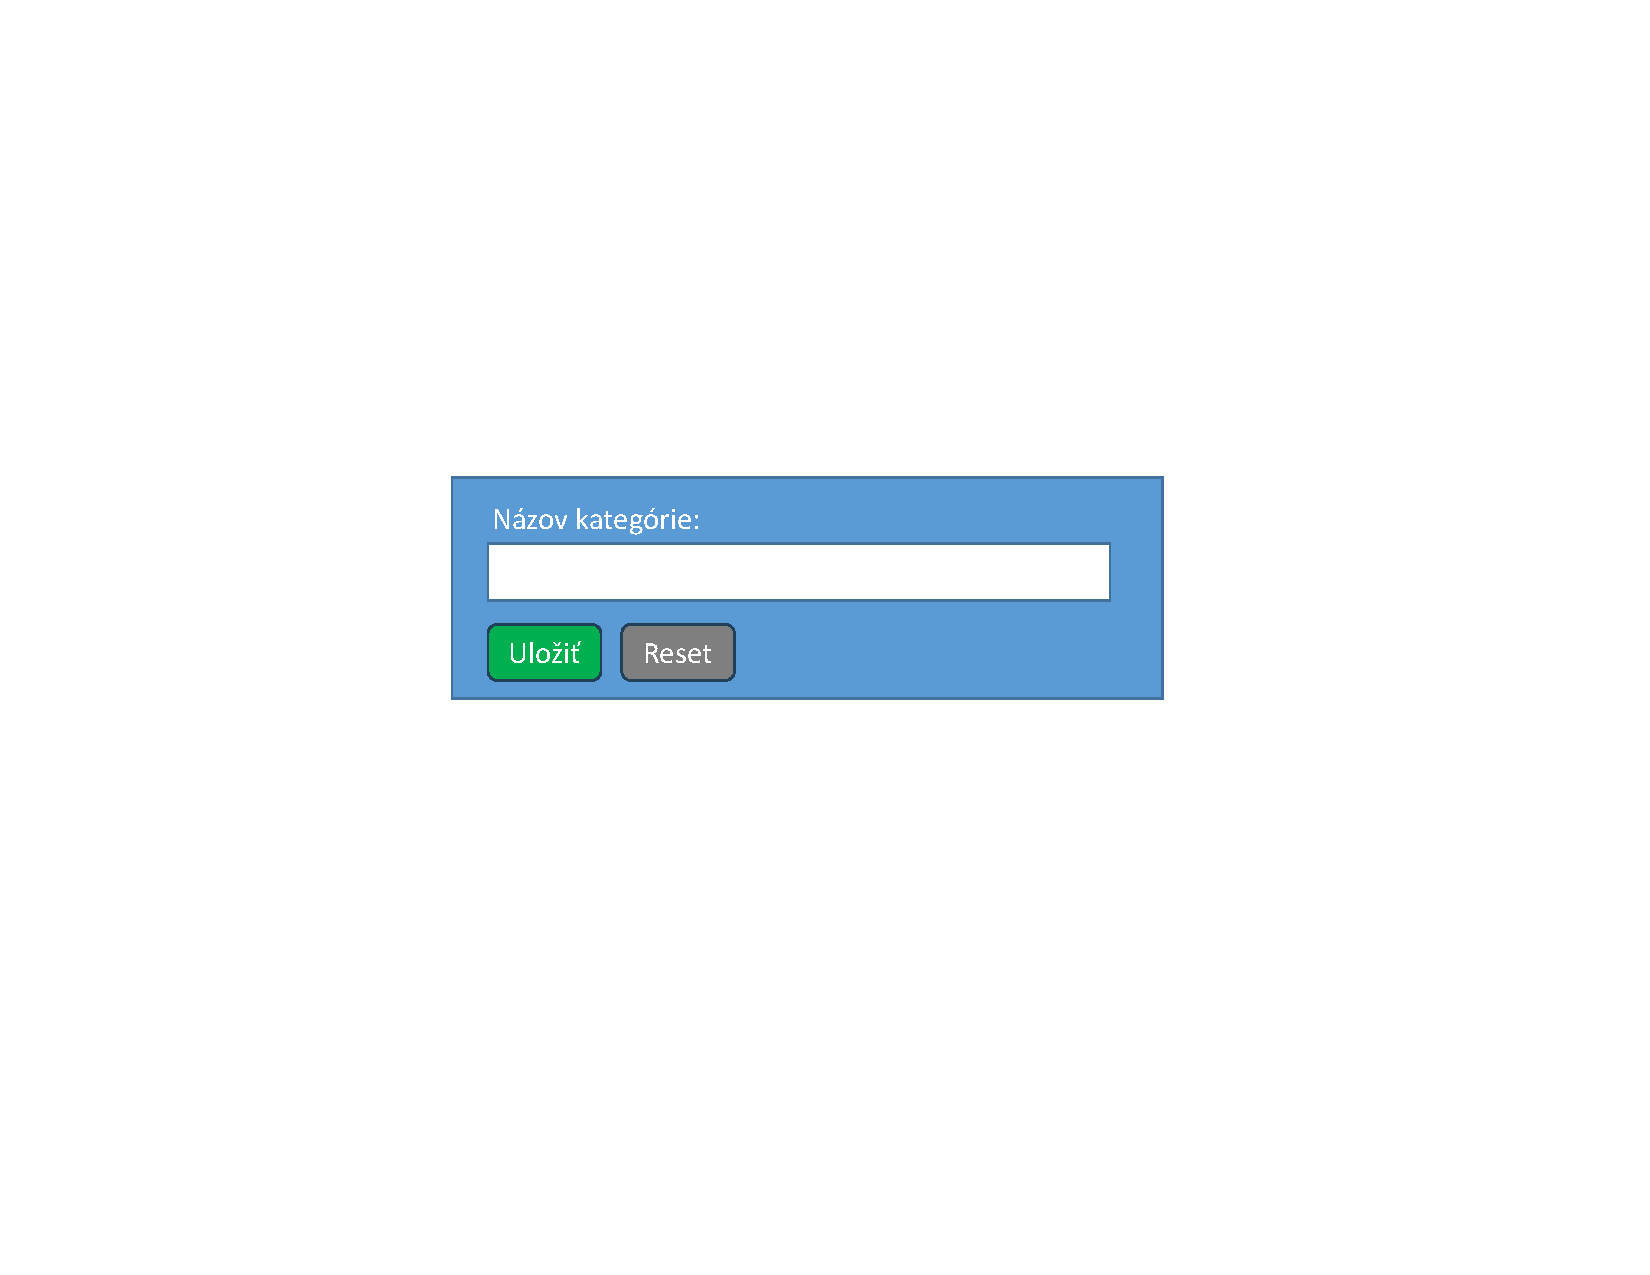
\includegraphics[width=140mm]{../img/UI concept/excavator category form}
\caption{Formulár kategórie bagra.}
\label{excavator category form}
\end{figure}

Formulár by mal obsahovať pole pre názov kategórie bagra (údaj je povinný). Ďalej by sa mali v spodnej časti formulára nachádzať tlačidlá \uv{Uložiť} (pre uloženie záznamu) a~\uv{Reset} (pre vyprázdenie formulára). Ak by bolo po~kliknutí na~tlačidlo \uv{Uložiť} pole prázdne, tak by na to mala aplikácia upozorniť odpovedajúcou chybovou správou.

\item \textit{Správa značiek bagrov}

Nad tabuľkou by sa mal nachádzať nadpis~\uv{Správa značiek bagrov}. V~tabuľke by mali byť stĺpce pre názov značky a~počet bagrov danej značky. Nemalo by sa dať vyhľadávať podľa počtu bagrov danej značky. Pre~lepšiu predstavu formulára pre vytvorenie, úpravu značky bagra viď~obr.~\ref{excavator brand form}.

\begin{figure}[H]\centering
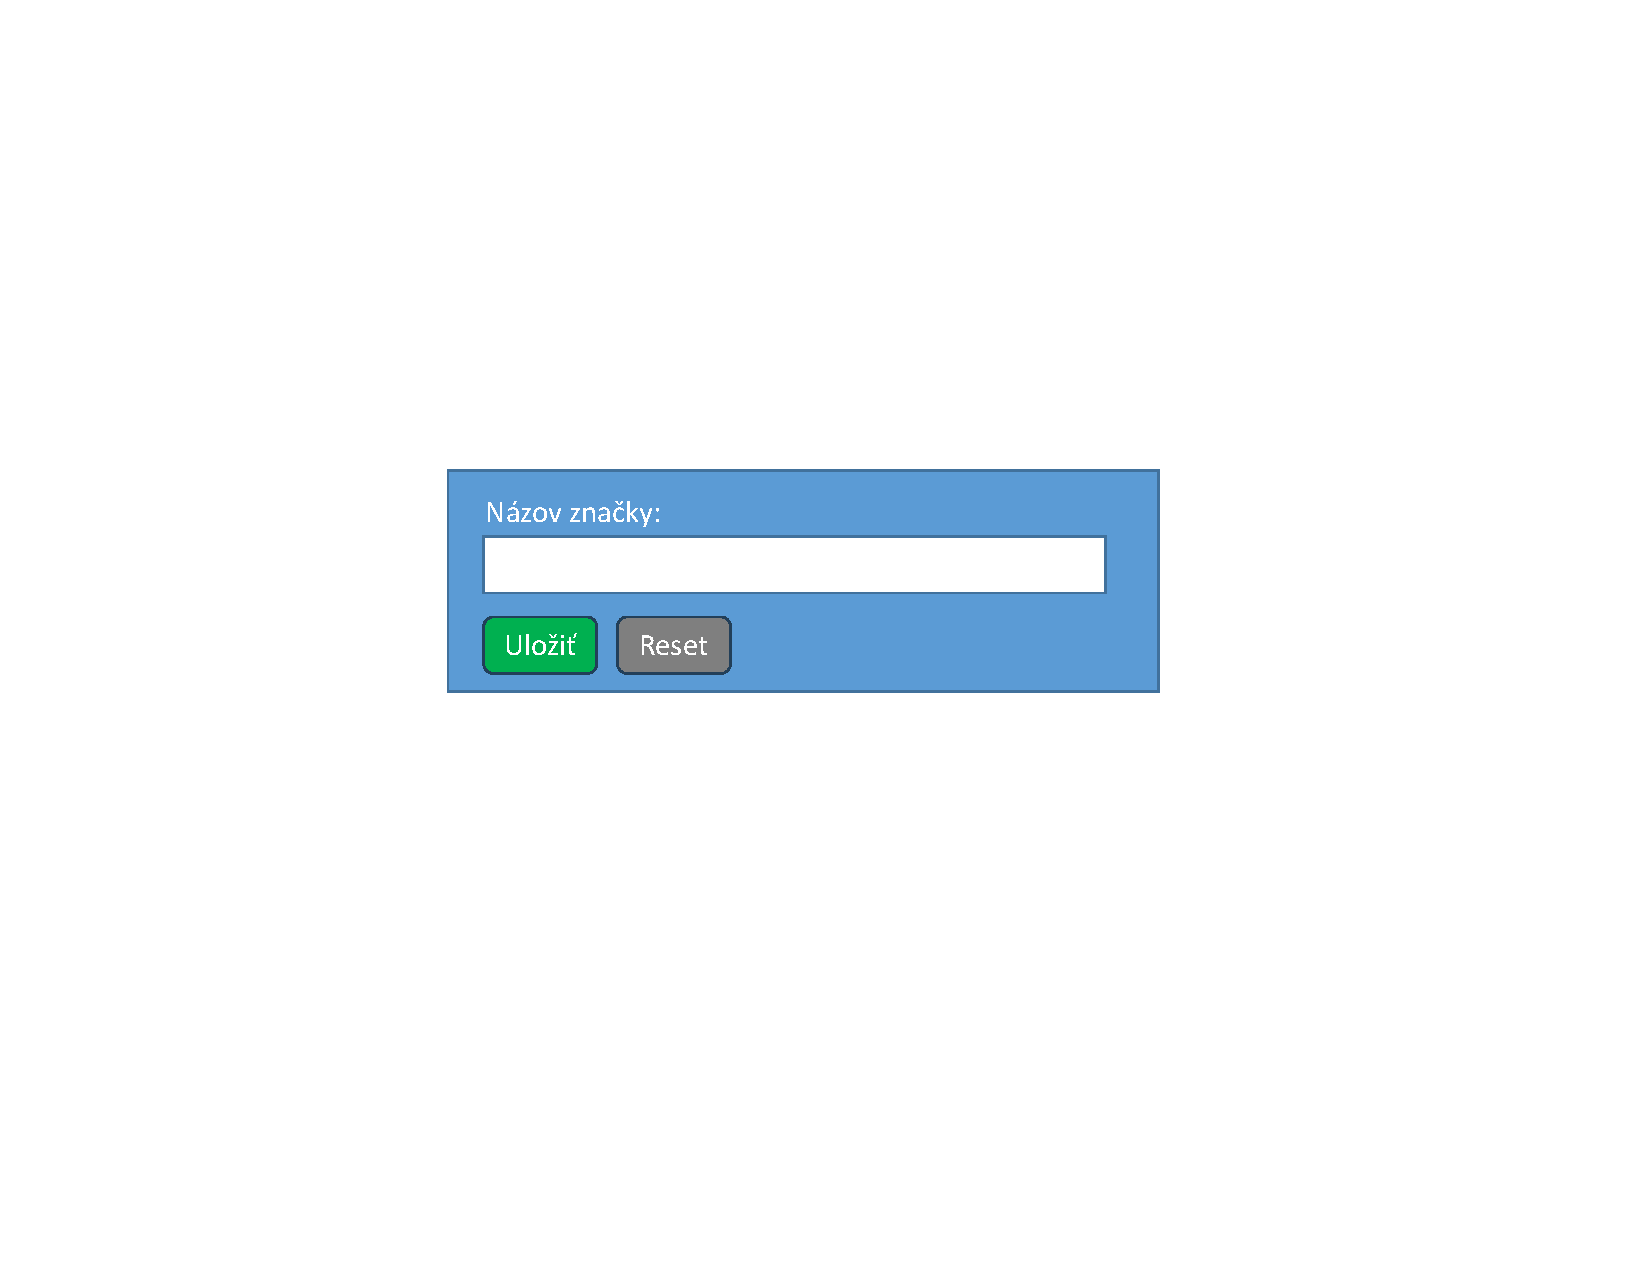
\includegraphics[width=140mm]{../img/UI concept/excavator brand form}
\caption{Formulár značky bagra.}
\label{excavator brand form}
\end{figure}

Formulár by mal obsahovať pole pre názov značky bagra (údaj je povinný). V~spodnej časti formulára by sa mali nachádzať tlačidlá \uv{Uložiť} (pre~uloženie záznamu) a~\uv{Reset} (pre vyprázdenie formulára). Ak by bolo po~kliknutí na~tlačidlo \uv{Uložiť} pole prázdne, tak by sa mala pri~poli zobraziť odpovedajúca chybová správa.
\end{itemize}

\item \textbf{Karta Kategórie a~značky prídavných zariadení}

Na karte Kategórie a~značky prídavných zariadení sa takisto nachádzajú dve tabuľky~-- jedna je pre~správu kategórií prídavných zariadení a~druhá pre~správu značiek prídavných zariadení. Taktiež si ich teraz obe opíšeme:

\begin{itemize}
\item \textit{Správa kategórií prídavných zariadení}

Nad tabuľkou by sa mal nachádzať nadpis~\uv{Správa kategórií prídavných zariadení}. Tabuľka by mala obsahovať stĺpce pre názov kategórie a~počet prídavných zariadení danej kategórie. Nemalo by sa dať vyhľadávať podľa počtu prídavných zariadení danej kategórie. Formulár pre~vytvorenie, úpravu kategórie prídavného zariadenia je totožný s formulárom pre~vytvorenie, úpravu bagra, a~preto pre~jeho lepšiu predstavu viď~obr.~\ref{excavator category form}.

\item \textit{Správa značiek prídavných zariadení}

Nad tabuľkou by sa mal nachádzať nadpis~\uv{Správa značiek prídavných zariadení}. V~tabuľke by mali byť stĺpce pre názov značky a~počet prídavných zariadení danej značky. Nemalo by sa dať vyhľadávať podľa počtu prídavných zariadení danej značky. Pre~lepšiu predstavu formulára pre~vytvorenie, úpravu značky bagra je možné pozrieť obr.~\ref{excavator brand form}, pretože tieto formuláre sú výzorovo a~správaním totožné.
\end{itemize}
\end{itemize}

\section{Splnenie P6}
\label{splnenie p6}

V~tejto podkapitole si prejdeme časti aplikácie spĺňajúce požiadavku P6, t.~j.~umožnenie užívateľom registrovať a~prihlásiť sa do~systému (pričom administrátori sa majú prihlasovať rovnakým spôsobom ako bežní zákazníci), umožnenie zmeny údajov v~profile, zjednodušenie prihláseným užívateľom vypĺňanie formulárov (aby nemuseli zadávať svoje osobné údaje), umožnenie neprihláseným užívateľom posielať dopyty a~účastniť sa aukčných dražieb.

V~častaiach~\ref{dopyt}, \ref{ponukanie sumy do drazby} a~\ref{splnenie p8} už bolo spomenuté, že aj prihlásení, aj neprihlásení užívatelia by mali byť schopní dopytovať sa na~bager, prídavné zariadenie, výkopovú službu alebo~takisto ponúkať sumy do~dražby (teda zapájať sa do~aukcie). Pričom prihláseným užívateľom by sa nemali zobrazovať polia s~osobnými údajmi (nemusia ich vypĺňať). Tým pádom sú požiadavky zjednodušenie vypĺňania formulárov prihlásenými užívateľmi, umožnenie posielania dopytov neprihláseným užívateľom a~umožnenie účasti v~aukcii neprihláseným užívateľom splnené.

\subsection{Prihlasovací panel}

\textbf{Spoločný pohľad:} V~ľavej časti aplikácie nad~navigáciou by sa mal nachádzať prihlasovací panel. Pre~lepšiu predstavu umiestnenia panela viď~obr~\ref{layout}) a~pre~lepšiu predstavu samotného panela, spolu s~prihlasovacím a~registračným formulárom, viď~obr.~\ref{auth}.

\begin{figure}[H]\centering
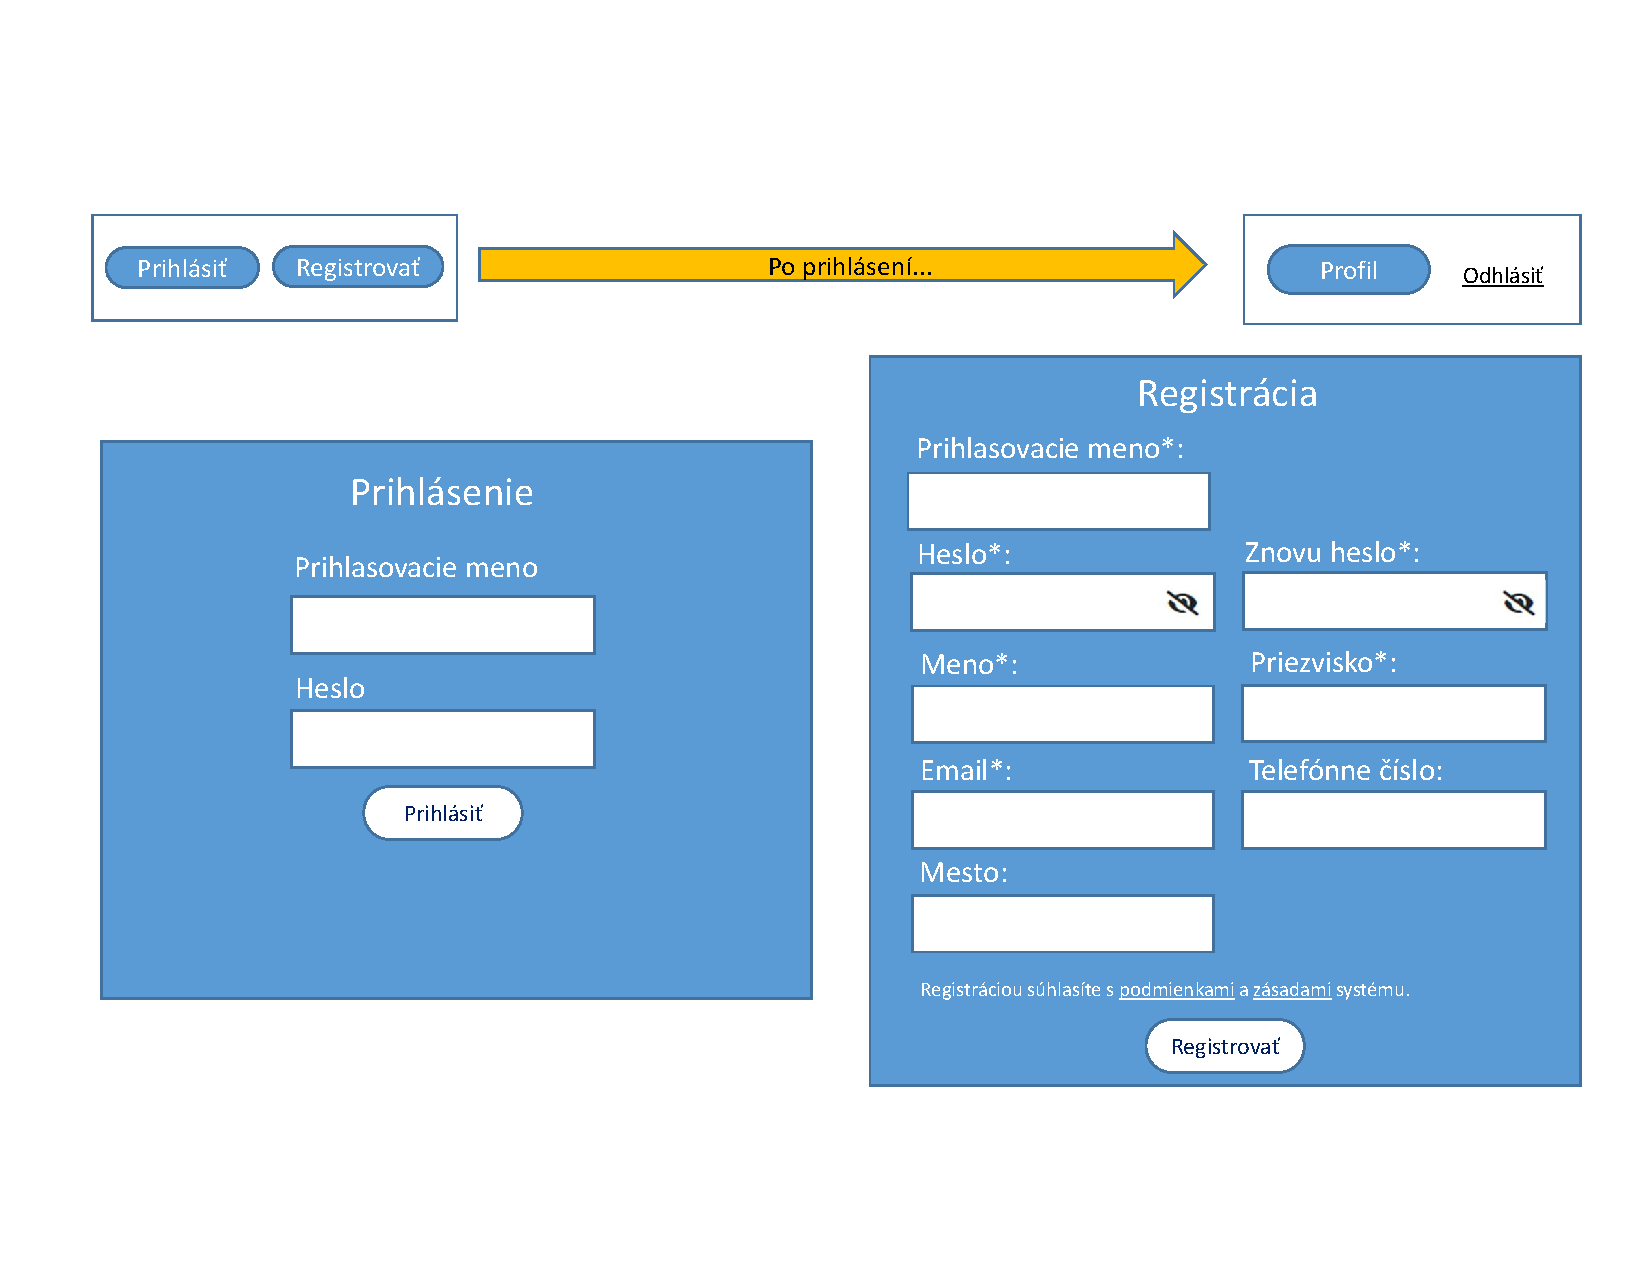
\includegraphics[width=140mm]{../img/UI concept/auth}
\caption{Prihlasovací panel (hore), prihlasovací formulár (vľavo), registračný formulár (vpravo).}
\label{auth}
\end{figure}

Prihlasovací panel by mal obsahovať:
\begin{itemize}
\item \textbf{Pre neprihláseného užívateľa:}
Tlačidlá~,,Prihlásiť`` a~,,Registrovať`` (viď~vľavo hore na~obr.~\ref{auth}). Po~kliknutí na~tlačidlo~,,Prihlásiť`` by mal byť užívateľ presmerovaný do~časti aplikácie s~prihlasovacím formulárom (viď~ľavú časť obr.~\ref{auth}). Po~kliknutí na~tlačidlo~,,Registrovať`` by mal byť užívateľ presmerovaný do~časti aplikácie s~registračným formulárom (viď~pravú časť obr.~\ref{auth}).
\item \textbf{Pre prihláseného užívateľa:}
Tlačidlo~,,Profil`` a~odkaz ,,Odhlásiť`` (viď~vpravo hore na~obr.~\ref{auth}). Po~kliknutí na~tlačidlo~,,Profil`` by mal byť užívateľ presmerovaný do~časti aplikácie s~jeho údajmi. Po~kliknutí na~odkaz~,,Odhlásiť`` by mal byť užívateľ odhlásený.
\end{itemize}

\subsection{Prihlásenie}
\label{prihlasenie}

\textbf{Pohľad pre~neprihlásených užívateľov:} Po kliknutí na~tlačidlo \uv{Prihlásiť} (ktoré by sa malo nachádzať v~prihlasovacom paneli) by sa mal užívateľ dostať do časti aplikácie s~formulárom pre~prihlásenie. Pre~lepšiu predstavu formulára viď ľavú časť obr. \ref{auth}.

Formulár by mal vo vrchnej časti obsahovať nadpis \uv{Prihlásenie}, pod ním polia pre prihlasovacie meno a heslo. Pod poliami by sa sa malo nachádzať tlačidlo \uv{Prihlásiť}. Ak by užívateľ zadal prihlasovacie meno, ktoré neexistuje (nie je evidované v systéme), malo by sa mu po kliknutí na tlačidlo \uv{Prihlásiť} zobraziť vyskakovacie okno s~textom~\uv{Užívateľ s takýmto menom neexistuje.} a~tlačidlom~,,OK``. Podobne ak by užívateľ zadal nesprávnu kombináciu prihlasovacieho mena a hesla, malo by sa mu po kliknutí na tlačidlo \uv{Prihlásiť} zobraziť vyskakovacie okno s~textom~\uv{Nesprávne heslo.} a~tlačidlom~,,OK``. Po vyplnení (validných) údajov a kliknutí na tlačidlo \uv{Prihlásiť} by mal byť užívateľ prihlásený do~systému a~presmerovaný do~sekcie Hlavná ponuka.

\subsection{Registrácia}
\label{registracia}

\textbf{Pohľad pre~neprihlásených užívateľov:} Po kliknutí na~tlačidlo \uv{Registrovať} by sa mal užívateľ dostať do časti aplikácie s~formulárom pre~registráciu. Pre~lepšiu predstavu formulára viď~pravú časť obr.~\ref{auth}.

V hornej časti formulára by sa mal nachádzať nadpis \uv{Registrácia}. Formulár by mal obsahovař povinné polia prihlasovacie meno, heslo, znova heslo, meno, priezvisko, email a nepovinné polia telefónne číslo a mesto. Ak by užívateľ začal písať do~poľa heslo alebo~znova heslo, namiesto písmen by sa mu mali zobrazovať hviezdičky. Pri~týchto poliach by mali byť ikonky pre zobrazenie/schovanie hesla. Ak by užívateľ klikol na ikonku, namiesto hviezdičiek by sa mu mali zobraziť písmená (opätovným kliknutím opäť hviezdičky). Teda išlo by o~funkcionalitu zobraziť a~schovať heslo. Formulár by mal takisto obsahovať upozornenie, že registráciou užívateľ súhlasí s podmienkami a zásadami systému. Upozornenie by malo zároveň odkazovať na časti aplikácie s podmienkami používania a so zásadami ochrany osobných údajov, ktoré boli spomenuté v podkap. \ref{gdpr}. V spodnej časti formulára by sa malo nachádzať tlačidlo \uv{Registrovať}, ktorým by sa užívateľ mal byť schopný zaregistrovať do systému. Po úspešnej registrácii by mal byť užívateľ presmerovaný do sekcie Hlavná ponuka.

Ak by po kliknutí na tlačidlo \uv{Registrovať} nebola hodnota nejakého z polí validná (napr. absencia hodnoty v povinnom poli), mala by sa pri takomto poli zobraziť vhodná chybová správa. Zároveň obsah políčok heslo a znova heslo by mal byť rovnaký. V prípade, že by rovnaký nebol a užívateľ by klikol na tlačidlo \uv{Registrovať}, tak by sa malo zobraziť vyskakovacie okno s~textom~\uv{Obsah políčok \'Heslo\' a \'Znova heslo\' nie sú rovnaké.} a~tlačidlom~,,OK``.

\subsection{Profil}
\label{profil}

\textbf{Spoločný pohľad:} Po~kliknutí na~tlačidlo~,,Profil``, ktoré by sa malo zobrazovať prihláseným užívateľom v~prihlasovacom paneli, by mal byť užívateľ presmerovaný do~časti aplikácie s~formulárom, ktorý by mal obsahovať jeho údaje. Užívateľ by mal byť schopný pomocou tohto formulára svoje údaje upravovať. Navyše nad~formulárom by sa mal nachádzať nadpis~,,Profil``. Pre~lepšiu predstavu tejto časti aplikácie viď~obr.~\ref{profile}.

\begin{figure}[H]\centering
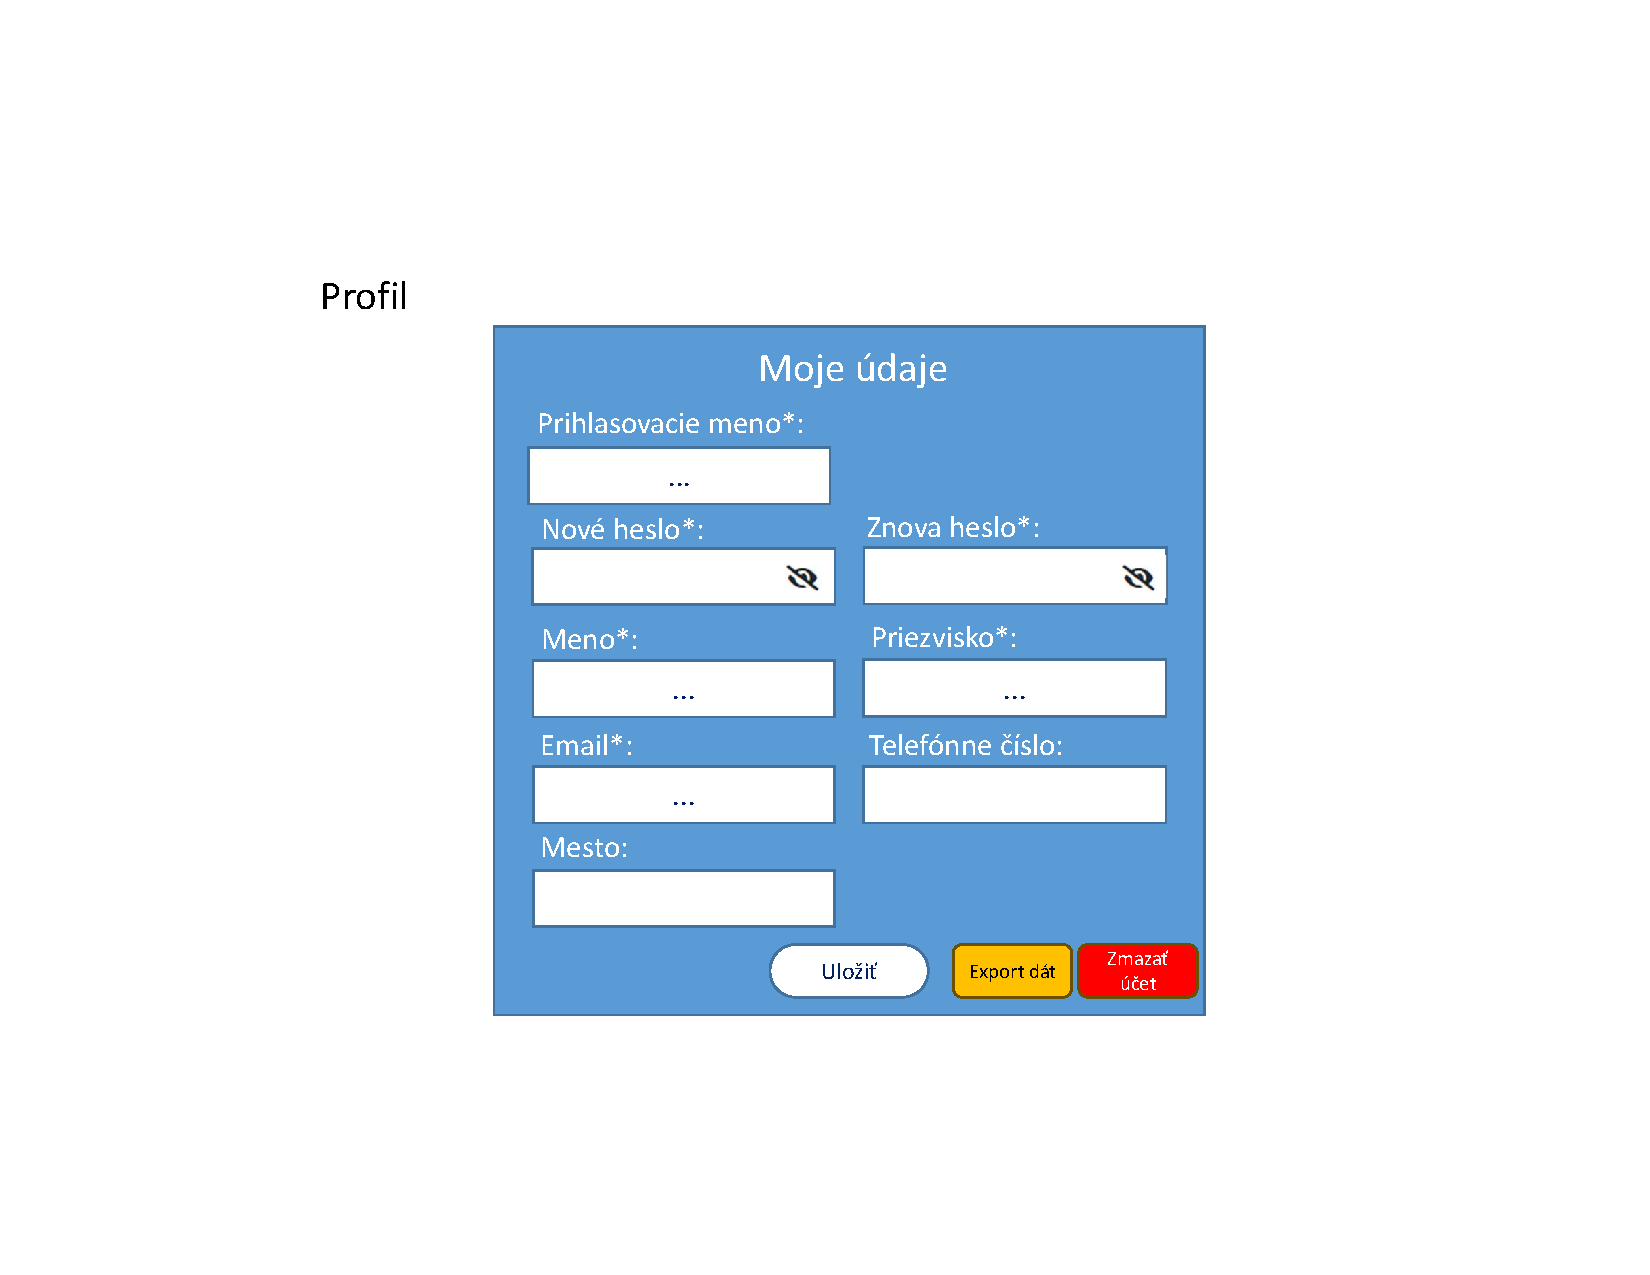
\includegraphics[width=140mm]{../img/UI concept/profile}
\caption{Profil užívateľa}
\label{profile}
\end{figure}

V~hornej časti formulára by sa mal nachádzať nadpis~,,Moje údaje``. Formulár by mal obsahovať polia prihlasovacie meno, heslo, znova heslo, meno, priezvisko, email, telefónne číslo a~mesto. Pričom všetky polia, okrem polí telefónne číslo a~mesto, sú povinné. Povinné polia by mali byť označené hviezdičkou.

Všetky polia, až na~polia heslo a~znova heslo, by mali byť vyplnené užívateľovými údajmi. Ak by užívateľ začal písať do~poľa heslo alebo~znova heslo, namiesto písmen by sa mu mali zobrazovať hviezdičky. Pri~týchto poliach by mali byť ikonky, ktoré by kliknutím umožnili užívateľovi meniť medzi hviezdičkami a~písmenami v~poliach heslo a~znova heslo. Teda išlo by o~funkcionalitu zobraziť a~schovať heslo.

Pod~formulárom by sa malo nachádzať tlačidlo~,,Uložiť`` pre~uloženie zmien. Ak by neboli vykonané žiadne zmeny, tak po~kliknutí na~tlačidlo~,,Uložiť`` by sa malo zobraziť vyskakovacie okno s~textom "Neboli vykonané žiadne zmeny." a~tlačidlom ,,OK``. Ak by užívateľ zinvalidoval nejaké z~polí (napr.~zanechá prázdne povinné pole), mala by sa zobraziť chybová správa pri~danom poli. Výnimkou sú polia heslo a~znova heslo~-- aj napriek tomu, že sú povinné, tak môžu ostať prázdne.

Ak by si chcel užívateľ zmeniť heslo, musel by vyplniť obe polia, a~ak by obsah polí nebol rovnaký, tak by sa malo zobraziť vyskakovacie okno s~textom~\uv{Obsah políčok \'Nové heslo\' a~\'Znova heslo\' nie sú rovnaké.} a~tlačidlom ,,OK``. Alebo ak by si chcel užívateľ zmeniť heslo a~zadal by staré heslo, tak znova by sa malo zobraziť vyskakovacie okno s~textom~\uv{Nové heslo nemôže byť staré heslo.} a~tlačidlom~,,OK``. Po úspešnej zmene údajov by sa malo zobraziť vyskakovacie okno s~textom~\uv{Údaje úspešne zmenené.} a~tlačidlom ,,OK``.

Okrem toho by sa mali v spodnej ľavej časti formulára nachádzať tlačidlá~\uv{Export dát} a~\uv{Zmazať účet}. Po~kliknutí na~tlačidlo~\uv{Export dát} by sa mali užívateľovi sťiahnuť údaje (v~textovej forme), ktoré má o ňom systém uložené. Po~kliknutí na~tlačidlo~\uv{Zmazať účet} by sa malo zobraziť modálne potvrdzovacie okno s~nadpisom~\uv{Vymazať svoj účet natrvalo} a~textom \uv{POZOR! Naozaj chcete vymazať svoj účet so všetkými svojimi dátami?}. Tieto obe tlačidlá by mali existovať z dôvodu prípravy na splnenie GPDR (spomenuté v podkap. \ref{gdpr}).
